% Default language option is [thaithesis]. The other possible option is [engthesis].
% Default format option is [ugrad]. Other possible options are [master,doctor].
\documentclass[a4paper]{ubu}
%\documentclass[a4paper,engthesis,master]{chula}

% List all required packages here
\usepackage{float}            % for floating figures
\usepackage{amsmath}            % for math related environment
\usepackage{amsfonts}           % fonts for math
\usepackage{listings}           % for psuedocode, lines of codes
\usepackage{caption}
\usepackage[labelformat=simple]{subcaption}
\renewcommand\thesubfigure{(\alph{subfigure})}    % for (a) in subcaption
\usepackage{enumitem}
\setlist{nolistsep,topsep=0pt}
\usepackage{graphicx}
\usepackage{wrapfig}            % for figures wrap inside text paragraph
\usepackage{pdfpages}           % for including pdf pages
\usepackage{verbatim}           % for block comment
\usepackage{multicol}

\usepackage{minted}

\usepackage{standalone}         % for proposal text inclusion
\usepackage{pgfgantt}           % for gantt chart
\usepackage{titlesec}
\titlespacing{\section}{0pt}{\parskip}{-\parskip}

\usepackage{array}
\usepackage{xcolor,colortbl}
\usepackage{pdflscape}
\usepackage{tabularx}
\usepackage{makecell}

\usepackage{rotating}

\newcommand*\rot{\rotatebox{90}}

% listings format
\lstset{
basicstyle=\ttfamily,
numbers=left,
numberstyle=\small,
breaklines=true,
xleftmargin=.1\linewidth,
frame=single,
columns=fullflexible,
captionpos=b,
showstringspaces=false
}

\usepackage{tikz}
\usetikzlibrary{shapes,positioning,arrows}

%%------------------------------------------------------------
%%-               SETTING THESIS PARAMETERS                  -
%%------------------------------------------------------------
\thesistitle                              % set the thesis tile (use {\wbr} for word break)
{แอปพลิเคชันสแกนอาหาร} % Thai Title
{Beingwellness}      % English title (auto upper case)

\authortitle                            % set the title of the author, e.g., Mr., Miss, Dr. etc.
{นาย}                                   % Thai Title of the author
{Mr.}                                   % English Title of the author
\thesisauthor                           % set the author name (must not include title (Mr., Miss, Dr., etc.)
{พัทธดนย์ จัยสิน}                          % Author name in Thai
{Pattadon Jaisin}                  % Author name in English

\advisor                                               % set the advisor
{อาจารย์ ดร.ไพชยนต์ คงไชย}               % Advisor name in Thai
{ดร. ไพชยนต์ คงไชย}                          % Advisor name in Thai with abbrev. title
{Phaichayon Kongchai, Ph.D.}  % Advisor name in English
{PHAICHAYON KONGCHAI, Ph.D.}          % Advisor name in English with abbrev. title 
                                                       % (Capital letters except Ph.D.))

%% If the thesis has co-advisor, use this optional command
%% Uncomment if necessary
%\coadvisor
%{อาจารย์ ดร.ภควรรณ ปักษี}  % Co-Advisor name in Thai
%{อ. ดร.ภควรรณ ปักษี}  % Co-Advisor name in Thai with abbrev. title
%{Pakawan Pucksee, Ph.D.}  % Co-Advisor name in English
%{PAKAWAN PUCKSEE, Ph.D.}          % Co-Advisor name in English with abbrev. title 
                                                       % (Capital letters except Ph.D.))

\faculty                                % set the faculty
{วิทยาศาสตร์}                          % name of the faculty in Thai
{Science}                           % name of the faculty in English
\department                             % set the department
{คณิตศาสตร์ สถิติ และคอมพิวเตอร์}                      % name of the department in Thai
{Mathematics Statistics and Computer}                  % name of the department in English
\fieldofstudy                           % set the field of study (สาขาวิชา)
{วิทยาการคอมพิวเตอร์}                      % Field in Thai
{Computer Science}                  % Field in English
\degree                                 % set the degree name
{วิทยาศาสตร์บัณฑิต}                   % Degree name in Thai
{Bachelor of Science}                  % Degree name in English
\academicyear{2561}                     % Academic Year (in Thai Calendar)
\authorid{5811403741}                   % ID of the author
\subjID{1104494}							% Course ID for undergrad report
\subjName								% course name
{โครงงานวิทยาศาสตร์2}
{Computer Project II}

\deanname                               % name of the dean
{ดร. ชัชวิน นามมั่น}                       % in Thai
{Chatchawin Namman, Ph.D.}     % in English

% Committee Block
% Speficy the chair/committee/external committee in your selected language
\committee                              % list of committee
{
\CommitteeBlockAdvisor                  % pre-defined value for advisor
\CommitteeBlockCoAdvisor                % pre-defined value for co-advisor
\CommitteeBlock{กรรมการ}{อาจารย์ วาสนา เหง้าเกษ } % examiner
\CommitteeBlock{กรรมการ}{ผศ. เกรียงศักดิ์ ตรีประพิณ}  % examiner
}

%%-------------------------------------------------------------------------------
%%-                               DOCUMENT                                      -
%%-------------------------------------------------------------------------------
\begin{document}
% Thesis starts with Thai Cover
\makethaicover
\newpage

% Followed by English Cover
%\makeenglishcover
%\newpage

% Generate committee page
\makecommittee
\newpage

% Acknowledgement Section
\begin{acknowledgements} %TODO update here!
	การพัฒนาโครงงานแอปพลิเคชันบีอิงเวลเนส สำเร็จลุล่วงได้ด้วยความกรุณาแลความช่วยเหลือจากหลายๆ ท่าน ข้าพเจ้าขอขอพระคุณทุกท่าน ที่มีส่วนร่วมในการพัฒนาโครงงานนี้
	
    ขอขอบพระคุณอาจารย์ที่ปรึกษา ดร. ไพชยนต์ คงไชย  อาจารย์ที่ปรึกษาโครงงานที่ได้แนะนำทฤษฎีและแนวทางในแก้ปัญหาต่าง ๆ  ที่เกิดขึ้นระหว่างการพัฒนาแอปพลิเคชัน อีกครั้งยังคอยตรวจสอบความก้าวหน้าของการทำงานเป็นระยะ ๆ รวมทั้งสร้างกำลังใจให้ผู้พัฒนาอยู่เสมอ
    
    ขอขอบพระคุณเจ้าหน้าที่ภาควิชาคณิตศาสตร์ สถิติและคอมพิวเตอร์ ที่คอยเอื้อยอำนวยความสะดวกทั้งเรื่องอุปกรณ์และสถานที่ต่อการปฏิบัติงานของผู้พัฒนา
   
    ขอกราบขอบพระคุณบิดา มารดา ที่คอยให้กำลังใจ คอยให้ความรักและความห่วงใยเสมอมา
    ตลอดจนคอยช่วยเหลือทุนทรัพย์ทางด้านการศึกษาและอุปกรณ์ในการพัฒนาโครงงาน

    
\end{acknowledgements}

\begin{flushright}
    นายพัทธดนย์ จัยสิน
    \vspace{-5mm}
    วันที่ 19 เมษายน 62
\end{flushright}

\newpage

% Thai Abstract Section
\begin{thaiabstract}
    Being-wellness เป็นแอพพลิเคชั่นที่วัดแคลลอรี่ ไขมัน น้ำตาล และโซเดียม จากอาหารที่
    รับประทานเพื่อทำนายความเสี่ยงของโรคที่เกิดจากการรับประทานอาหาร ผู้ใช้สามารถถ่ายรูปอาหารเพื่อเก็บ
    ข้อมูลด้วยการใช้เทคนิคการตรวจจับวัตถุแล้วนำผลลัพธ์ที่ได้ไปเทียบกับฐานข้อมูลจากนั้นนำข้อมูลอาหารที่
    ได้มาแสดง ในแอพพลิเคชั่นนี้ได้ใช้การเรียนรู้เชิงลึกและใช้ขั้นตอนวิธีMobilenet v1 1.0 เพื่อตรวจจับอาหาร
    จากรูปภาพ ผู้จัดทำได้เลือกรูปภาพอาหารที่แตกต่างกัน 50 รูปโดยเลือกใช้สินค้าที่มียอดขายดีสุดจากร้านค้า
    เซเว่น-อีเลฟเว่น เพื่อเป็นชุดข้อมูลฝึกฝน จากการทดลองพบว่ามีค่าความถูกต้องอยู่ที่ร้อยละ 78.8 จาก
    รูปภาพอาหาร 100 รูป
\noindent
\\คำสำคัญ: สมาร์ทโฟน, แอพพลิเคชั่น, เทคนิคการตรวจจับวัตถุ, การเรียนรู้เชิงลึก, Mobilenet v1 1.0,
ฐานข้อมูล
\end{thaiabstract}

\newpage

% English Abstract Section
\begin{englishabstract}
    Being-wellness is an smartphone application that determines calorie, fat, sugar and sodium
    from the food you are eating daily for predict risk diseases from your food consumption.
    Users can take a food photo to record data based on the object detection technique
    And bring the results compared to the database, then bring the food information that has
    been shown. In this application , we used deep learning algorithm named Mobilenet v1 1.0
    for detect foods from photo, we collected 50 different food photos in best seller from
    seven-eleven supermarket for training model. The experimental results showed that 78.8%
    percent of 100 of food photos were correctly detected.


\noindent
Keywords: Smartphone Application, Object Detection Technique, Deep Learning Algorithm,
Mobilenet v1 1.0, Database
\end{englishabstract}


\newpage


% Table of Content
\tableofcontents        % generate table of content
\newpage
\listoftables           % generate list of tables
\newpage
\listoffigures          % generate list of figures
\newpage

% Main Content
\chapter{บทนำ}

\section{ที่มาและเหตุผล }
ทุกวันนี้ประเทศไทยมีอาหารที่หลากหลาย แต่อาหารบางชนิดยังมีการปรุงอาหารรสจัดมากจนเกินไป ทำให้ร่างกายได้รับสารอาหารมากเกินความจำเป็น ส่งผลให้ร่างกายเกิดโรคตามมา เช่น การปรุงอาหารรสเค็มจัด ก็จะทำให้ผู้บริโภคมีความเสี่ยงต่อการเป็นโรคไต จึงมีการพัฒนาแอปพลิเคชันมาใช้ในการจัดเก็บข้อมูลการบริโภคทำให้สามารถควบคุมไม่ให้มีการบริโภคเกินความจำเป็นของร่างกาย แต่แอปพลิเคชันยังมีข้อเสียคือ แอปพลิเคชันจะต้องมีการซื้อเพื่อที่จะสามารถใช้งานได้เต็มประสิทธิภาพและยังมีความซับซ้อนในการบันทึกข้อมูลการบริโภค

แต่ในปัจจุบันมีการนำปัญญาประดิษฐ์(Artificial Intelligence:AI) มาใช้ประโยชน์อย่างแพร่หลาย ไม่ว่าจะเป็นทางด้านการแพทย์เพื่อช่วยในการวินิจฉัยโรค ด้านการคมนาคมช่วยมาการมาช่วยในการควบคุมการทำงานของยานพาหะนะหรือด้านการเกษตรที่ช่วยในการควบคุมระบบน้ำและอุณหภูมิ แต่ทางด้านอาหารยังไม่มีการนำมาใช้มากนัก 

ผู้พัฒนาจึงเล็งเห็นปัญหาดังกล่าวจึงได้ทำการพัฒนาแอปพลิเคชันจัดเก็บข้อมูลการบริโภคงานวิจัยนี้ได้มีการนำปัญญาประดิษฐ์มาช่วยในการบันทึกข้อมูลการบริโภคโดยระบบจำทำการเรียนรู้ภาพที่ทำการถ่ายเข้ามาแล้วนำมาประมวลผลเพื่อระบุข้อมูลอาหารจากภาพถ่าย งานวิจัยนี้ได้นำเทคนิคทางด้านการประมวลผลภาพ(Image Processing) และเทคนิคการเรียนรู้ของเครื่อง (Machine Learning) มาใช้ในการตรวจจับอาหาร



\section{วัตถุประสงค์}
\begin{enumerate}
	\item เพื่อพัฒนาแอพพลิเคชั่นสแกนอาหารสำหรับเก็บและแสดงข้อมูลการบริโภคอาหาร 
	\item  เพื่อสามารถบอกชื่ออาหารที่ทำการสแกนได้อย่างแม่นยำ  
\end{enumerate}
% \section{ขอบเขตของโครงงาน}
% \begin{enumerate}[label=1.3.\arabic*]
% 	\begin{enumerate}
% 		\item ใช้ภาพถ่ายอาหาร ที่ขายดีในเซเว่น อีเลฟเว่น จำนวน 50 ชนิด เพื่อใช้ในการฝึกสอน(train)
% 		\item อาหารแต่ละชนิดจะใช้ภาพถ่ายจำนวน 100 รูป

% 	\end{enumerate}
% \end{enumerate}


\newpage

\section{ขอบเขตของโครงงาน}
\begin{enumerate}
	\item ใช้ภาพถ่ายอาหาร ที่ขายดีในเซเว่น อีเลฟเว่น จำนวน 50 ชนิด เพื่อใช้ในการฝึกสอน(train)
		\item อาหารแต่ละชนิดจะใช้ภาพถ่ายจำนวน 100 รูป 
\end{enumerate}
\section{ประโยชน์ที่คาดว่าจะได้รับ}
\begin{enumerate}
	\item ผู้ใช้ได้รับความสะดวกในการเก็บข้อมูลการบริโภคของตนเอง 
	\item ผู้ใช้มีการบริโภคอาหารที่ดีขึ้น
  \item เป็นการวิจัยที่สามารถนำไปต่อยอดได้โดยการเพิ่มฟังก์ชันการออกกำลังการเพื่อให้มีการดูแลสุขภาพทั้งทางด้านการกินและการออกกำลังกาย 
\end{enumerate}
\section{เครื่องมือที่ใช้ในการพัฒนา (Development tools)}
\subsection{ฮาร์ดเเวร์}
\begin{enumerate}
	\item สมาร์ทโฟน (Smart phone)
		\begin{itemize}
			\item ระบบปฏิบัติการเวอร์ชัน 9.0 หรือ API Level 21
			\item หน่วยประมาลผลกลาง Qualcomm Snapdragon 660 AIE Octa Core ความเร็ว 2.2 กิกะเฮิร์ตซ์ (Gigahertz, GHz)
			\item หน่วยความจำหลักอย่างน้อย 4 กิกะไบต์ (Gigabyte, GB)
			\item หน่วยความจำสำรองอย่างน้อย 32 กิกะไบต์ (Gigabyte, GB)
			\item หน้าจอแสดงผลความละเอียดอย่างน้อย 2160 x 1080 พิกเซล  (Pixel)
			\item หน้าจอแสดงผลขนาดอย่างน้อย 5.99 นิ้ว
			\item กล้องถ่ายรูปความละเอียดอย่างน้อย 20 เมกกะพิกเซล (Magapixel)
		\end{itemize}
	
	\item เครื่องคอมพิวเตอร์ส่วนบุคคล (Personal computer)
		\begin{itemize}
			\item  	ระบบปฏิบัติการ macOS mojave 
			\item  หน่วยประมวลผลกลาง(cpu) Intel Core i5  ความเร็ว 2.3 กิกะเฮิร์ตซ์ (Gigahertz, GHz)
			\item  หน่วยประมวลผลกราฟฟิก Intel Iris Plus Graphics 640 ความจำ 1.5 กิกะไบต์ (Gigabyte, GB) 
			\item  หน่วยความจำหลัก 8 กิกะไบต์ (Gigabyte, GB)
			\item  หน่วยความจำสำรอง 256 กิกะไบต์ (Gigabyte, GB)
		\end{itemize}
\end{enumerate}

\subsection{ซอฟต์แวร์ (Software)}
\begin{enumerate}
	\item Java เป็นภาษาโปรแกรมที่ใช้ในการพัฒนา 
	\item Android Studio เป็น IDE (Integrated Development Environment) ใช้พัฒนาแอปพลิเคชันสำหรับระบบปฏิบัติการแอนดรอยด์
	\item Tensorflow Lite เป็น Libary ใช้ในการสร้างโมเดล ในการทำ Machine Learning 
\end{enumerate}

\newpage
\subsection{แผนการดำเนินการ}
	ในการพัฒนาแอปพลิเคชันสแกนอาหาร ผู้พัฒนาได้แบ่งขั้นตอนการดำเนินงานไว้ด้วยกัน 8 ขั้นตอน ดังต่อไปนี้

%\begin{landscape}
%\sffamily
\begin{table}[H]
	\noindent
	\caption{ขั้นตอนการดำเนินงาน}
	\begin{ganttchart}[
		canvas/.append style={fill=none, draw=black!5, line width=.75pt},
		vgrid={*2{draw=black!7, line width=.75pt}},
		title label font=\bfseries\footnotesize,
		bar label node/.append style={
			align=left,
			text width=width("7. Functional Testing On")},
		bar/.append style={draw=none, fill=black!63}
		]{1}{18}
		\gantttitle{2561}{6}
		\gantttitle{2562}{12}\\
		\gantttitle{พ.ย.}{3}
		\gantttitle{ธ.ค.}{3}
		\gantttitle{ม.ค.}{3}
		\gantttitle{ก.พ.}{3} 
		\gantttitle{มี.ค.}{3}
		\gantttitle{เม.ย.}{3} \\
		\ganttbar{1.ศึกษาความเป็นไปได้}{1}{6} \\
		\ganttbar{2.เสนอหัวข้อโครงงาน}{1}{3} \\
		\ganttbar{3.ศึกษาค้นคว้าข้อมูล}{3}{6} \\
		\ganttbar{4.ศึกษาการใช้เครื่องมือ}{1}{6} \\
		\ganttbar{5.วิเคราะห์และออกแบบ}{6}{9} \\
		\ganttbar{6.เขียนโปรแกรม}{6}{15} \\
		\ganttbar{7.ทดสอบและแก้ปัญหา}{10}{16} \\
		\ganttbar{8.จัดทำเอกสาร}{17}{18} \\
	\end{ganttchart}
	\label{tab:ganttchart}
\end{table}
%\end{landscape}
%TODO แก้เทมเพลตเอาชื่อตารางไว้ด้านบน
 
\chapter{ทฤษฎีที่เกี่ยวข้อง}
บทนี้จะเป็นรายละเอียดเกี่ยวกับทฤษฎีและงานวิจัยที่เกี่ยวของกับการพัฒนาแอปพลิเคชันในครั้งนี้ โดยแบ่งเนือหาออกเป็น ส่วนได้แก่ ส่วนที่ 1 เครื่องมือที่ใช้ในการพัฒนาแอปพลิเคชัน หัวข้อที่ (2.1) ส่วนที่ 2 ความรู้ภาษาที่ใช้ในการพัฒนาระบบ หัวข้อที่ (2.2-2.3) 
ส่วนที่ 3 ความรู้ของ Library ที่มช้พัฒนาแอปพลิเคชัน หัวข้อที่ (2.4-2.6) ส่วนที่ 4 ความรู้ฐานข้อมูลที่ใช้พัฒนาแอปพลิเคชัน หัวข้อที่ (2.7) 
% \begin{enumerate}[label=2.\arabic*]
% 	\item ความรู้พื้นฐานระบบปฏิบัติการแอนดรอยด์
% 	\item ความรู้พื้นฐานภาษา Java
% 	\item ความรู้พื้นฐานภาษา Python
% 	\item ความรู้พื้นฐาน Tensorflow Lite
% 	\item ความรู้พื้นฐานของระบบ XX เดิม
% 	\item เอกสารและงานวิจัยที่เกี่ยวข้อง
% \end{enumerate}

\section{ความรู้พื้นฐานระบบปฏิบัติการแอนดรอยด์}
	แอนดรอยด์ \cite{bib1} แอนดรอยด์ (Android) คือระบบปฏิบัติการแบบเปิดเผยซอร์ฟแวร์ต้นฉบับ (Open Source) โดยบริษัท กูเกิ้ล (Google Inc.) ที่ได้รับความนิยมเป็นอย่างสูง เนื่องจากอุปกรณ์ที่ใช้ระบบปฏิบัติการแอนดรอยด์ มีจำนวนมาก อุปกรณ์มีหลากหลายระดับ หลายราคา รวมทั้งสามารถทำงานบนอุปกรณ์ที่มีขนาดหน้าจอ และความละเอียดแตกต่างกันได้ ทำให้ผู้บริโภคสามารถเลือกได้ตามต้องการ

	และหากมองในทิศทางสำหรับนักพัฒนาโปรแกรม (Programmer) แล้วนั้น การพัฒนาโปรแกรมเพื่อใช้งานบนระบบปฏิบัติการแอนดรอยด์ ไม่ใช่เรื่องที่ยาก เพราะมีข้อมูลในการพัฒนารวมทั้ง Android SDK (Software Development Kit) เตรียมไว้ให้กับนักพัฒนาได้เรียนรู้ และเมื่อนักพัฒนาต้องการจะเผยแพร่หรือจำหน่ายโปรแกรมที่พัฒนาแล้วเสร็จ แอนดรอยด์ก็ยังมีตลาดในการเผยแพร่โปรแกรม ผ่าน Android Market แต่หากจะกล่าวถึงโครงสร้างภาษาที่ใช้ในการพัฒนานั้น สำหรับ Android SDK จะยึดโครงสร้างของภาษาจาวา (Java language) ในการเขียนโปรแกรม เพราะโปรแกรมที่พัฒนามาได้จะต้องทำงานอยู่ภายใต้ Dalvik Virtual Machine เช่นเดียวกับโปรแกรมจาวา ที่ต้องทำงานอยู่ภายใต้ Java Virtual Machine (Virtual Machine เปรียบได้กับสภาพแวดล้อมที่โปรแกรมทำงานอยู่)
	
	
	
%	\begin{figure}[H]
%		\centering
%		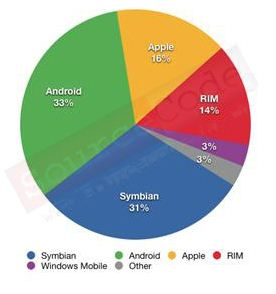
\includegraphics[width=0.5\columnwidth]{Figures/2/maketshare}
%		\caption{ส่วนแบ่งการตลาดระบบปฏิบัติการบนสมาร์ทโฟน}{ที่มา :  https://beerkung.wordpress.com/ระบบปฏิบัติการรุ่นล่าส/ระบบปฏิบัติการ-android.html}
%		\label{Fig:maketshare}
%	\end{figure}
\newpage
	\subsection{ประวัติความเป็นมาของระบบปฏิบัติการแอนดรอยด์}
ถูกพัฒนามาจากบริษัท แอนดรอยด์ (Android Inc.) เมื่อปี พ.ศ 2546 โดยมีนาย แอนดี้ รูบิน (Andy Rubin) ผู้ให้กำเนิดระบบปฏิบัติการนี้ และถูกบริษัท กูเกิ้ล ซื้อกิจการเมื่อ เดือนสิงหาคม ปี พ.ศ 2548 โดยบริษัทแอนดรอยด์ ได้กลายเป็นมาบริษัทลูก ของบริษัทกูเกิ้ล และยังมีนาย แอนดี้ รูบิน ดำเนินงานอยู่ในทีมพัฒนาระบบปฏิบัติการต่อไป
ระบบปฏิบัติการแอนดรอยด์ เป็นระบบปฏิบัติการที่พัฒนามาจากการนำเอา แกนกลางของระบบปฏิบัติการลินุกซ์ (Linux Kernel) ซึ่งเป็นระบบปฏิบัติการที่ออกแบบมาเพื่อทำงานเป็นเครื่องให้บริการ (Server) มาพัฒนาต่อ เพื่อให้กลายเป็นระบบปฏิบัติการบนอุปกรณ์พกพา (Mobile Operating System)
ต่อมาเมื่อเดือน พฤศจิกายน ปี พ.ศ 2550 บริษัทกูเกิ้ล ได้ทำการก่อตั้งสมาคม OHA (Open Handset Alliance) เพื่อเป็นหน่วยงานกลางในการกำหนดมาตรฐานกลาง ของอุปกรณ์พกพาและระบบปฏิบัติการแอนดรอยด์ โดยมีสมาชิกในช่วงก่อนตั้งจำนวน 34 รายเข้าร่วม ซึ่งประกอบไปด้วยบริษัทชั้นนำที่ดำเนินธุรกิจด้าการสื่อสาร เช่น โรงงานผลิตอุปกรณ์พกพา, บริษัทพัฒนาโปรแกรม, ผู้ให้บริการสื่อสาร และผู้ผลิตอะไหล่อุปกรณ์ด้านสื่อสาร \cite{bib2}
% 	\subsection{โครงสร้างของระบบปฏิบัติการแอนดรอยด์}
% 	การทำความเข้าใจโครงสร้างของระบบปฏิบัติการแอนดรอยด์ \cite{androidbook1} ถือว่าเป็นสิ่งสำคัญเพราะถ้านักพัฒนาโปรแกรม สามารถมองภาพโดยรวมของระบบได้ทั้งหมด จะสามารถเข้าใจถึงกระบวนการทำงานได้ดียิ่งขึ้น และสามารถนำไปช่วยในการออกแบบโปรแกรมที่ต้องการพัฒนาเพื่อให้เกิดประสิทธิภาพในการทำงาน
	
% 	\begin{figure}[H]
% 		\centering
% 		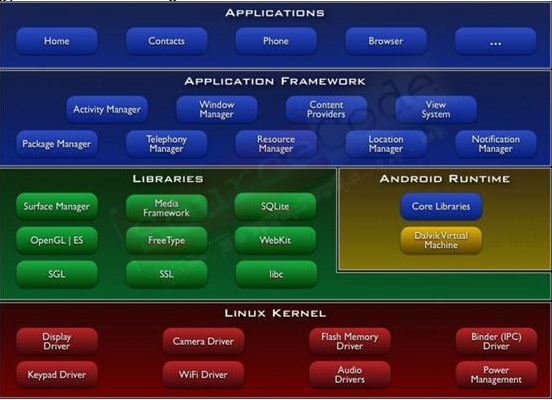
\includegraphics[width=0.8\columnwidth]{Figures/2/androidarchitecture}
% 		\caption{โครงสร้างของระบบปฏิบัติการแอนดรอยด์}{ที่มา : https://www.theandroid-mania.com/android-architecture/}
% 		\label{Fig:androidarchitecture}
% 	\end{figure}
% 	จากโครงสร้างของระบบปฏิบัติการแอนดรอยด์ในรูปที่ \ref{Fig:androidarchitecture} จะสังเกตได้ว่า มีการแบ่งออกเป็นส่วน ๆ ที่มีความเกี่ยวเนื่องกัน โดยส่วนบนสุดเป็นส่วนที่ผู้ใช้งานทำการติดต่อโดยตรงซึ่งคือส่วนของ Applications ลำดับถัดมาเป็นองค์ประกอบอื่น ๆ ตามลำดับ และสุดท้ายเป็นส่วนที่ติดต่อกับอุปกรณ์โดยผ่านทาง Linux Kernel โครงสร้างของแอนดรอยด์สามารถอธิบายได้ดังนี้

% 	\begin{enumerate}
% 		\item Applications ส่วนแอปพลิเคชันหรือส่วนของโปรแกรมที่มากับระบบปฏิบัติการ หรือเป็นกลุ่มของโปรแกรมที่ผู้ใช้งานได้ทำการติดตั้งไว้ โดยผู้ใช้งานสามารถเรียกใช้โปรแกรมต่าง ๆ ได้โดยตรงซึ่งการทำงานของแต่ละโปรแกรมจะเป็นไปตามที่ผู้พัฒนาโปรแกรมได้ออกแบบและเขียนโค้ด (Code) โปรแกรมเอาไว้
% 		\item Application Framework  เป็นส่วนที่มีการพัฒนาขึ้นเพื่อให้นักพัฒนาสามารถพัฒนาโปรแกรมได้สะดวก และมีประสิทธิภาพมากยิ่งขึ้น โดยนักพัฒนาไม่จำเป็นต้องพัฒนาในส่วนที่มีความยุ่งยากมากๆ เพียงแค่ทำการศึกษาถึงวิธีการเรียกใช้งาน Application Framework ในส่วนที่ต้องการใช้งานแล้วนำมาใช้งาน ซึ่งมีหลายกลุ่มด้วยกัน ตัวอย่างเช่น
% 			\begin{itemize}
% 				\item Activities Manager เป็นกลุ่มของชุดคำสั่งที่จัดการเกี่ยวกับวงจรการทำงานของหน้าต่างโปรแกรม (Activity)
% 				\item Content Providers เป็นกลุ่มของชุดคำสั่ง ที่ใช้ในการเข้าถึงข้อมูลของโปรแกรมอื่น และสามารถแบ่งปันข้อมูลให้โปรแกรมอื่นเข้าถึงได้
% 				\item View System เป็นกลุ่มของชุดคำสั่งที่เกี่ยวกับการจัดการโครงสร้างของหน้าจอที่แสดงผลในส่วนที่ติดต่อกับผู้ใช้งาน (User Interface)
% 				\item Telephony Manager เป็นกลุ่มของชุดคำสั่งที่ใช้ในการเข้าถึงข้อมูลด้านโทรศัพท์ เช่น หมายเลขโทรศัพท์ เป็นต้น
% 				\item Resource Manager เป็นกลุ่มของชุดคำสั่งในการเข้าถึงข้อมูลที่เป็นข้อความและรูปภาพ
% 				\item Location Manager เป็นกลุ่มของชุดคำสั่งที่เกี่ยวกับตำแหน่งทางภูมิศาสตร์ที่ระบบปฏิบัติการได้รับค่าจากอุปกรณ์
% 				\item Notification Manager เป็นกลุ่มของชุดคำสั่งที่จะถูกเรียกใช้เมื่อโปรแกรมต้องการแสดงผลให้กับผู้ใช้งาน ผ่านทางแถบสถานะ (Status Bar) ของหน้าจอ
% 			\end{itemize}
% 		\item Libraries เป็นส่วนของชุดคำสั่งที่พัฒนาด้วย C/C++ โดยแบ่งชุดคำสั่งออกเป็นกลุ่มตามวัตถุประสงค์ของการใช้งาน เช่น Surface Manage จัดการเกี่ยวกับการแสดงผล Media Framework จัดการเกี่ยวกับการการแสดงภาพและเสียง Open GL|ES และ SGL จัดการเกี่ยวกับภาพ 3 มิติ และ 2 มิติ SQLlite จัดการเกี่ยวกับระบบฐานข้อมูล เป็นต้น
% 		\item Android Runtime จะมี Darvik Virtual Machine ที่ถูกออกแบบมาเพื่อให้ทำงานบนอุปกรณ์ที่มีหน่วยความจำ (Memmory) หน่วยประมวลผลกลาง (CPU) และพลังงาน (Battery) ที่จำกัดซึ่งการทำงานของ Darvik Virtual Machine จะทำการแปลงไฟล์ที่ต้องการทำงานไปเป็นไฟล์ .DEX ก่อนการทำงานเหตุผลเพื่อให้มีประสิทธิภาพเพิ่มขึ้นเมื่อใช้งานกับหน่วยประมวลผลกลางที่มีความเร็วไม่มากส่วนต่อมาคือ Core Libraries ที่เป็นส่วนรวบรวมคำสั่งและชุดคำสั่งสำคัญโดยถูกเขียนด้วยภาษาจาวา (Java Language)
% 		\item Linux Kernel เป็นส่วนที่ทำหน้าที่หัวใจสำคัญในจัดการกับบริการหลักของระบบปฏิบัติการ เช่น เรื่องหน่วยความจำ พลังงาน ติดต่อกับอุปกรณ์ต่างๆ ความปลอดภัย เครือข่าย โดยแอนดรอยด์ได้นำเอาส่วนนี้มาจากระบบปฏิบัติการลินุกซ์ รุ่น 2.6 (Linux 26. Kernel) ซึ่งได้มีการออกแบบมาเป็นอย่างดี
% 	\end{enumerate}
% %	\subsection{ข้อเด่นของระบบปฏิบัติการแอนดรอยด์}
% %	เนื่องจากระบบปฏิบัติการแอนดรอยด์มีการเจริญเติบโตอย่างรวดเร็วและมีส่วนแบ่งตลาดของอุปกรณ์ด้านนี้ขึ้นทุกขณะ ทำให้กลุ่มผู้ใช้งานและกลุ่มนักพัฒนาโปรแกรมให้ความสำคัญกับระบบปฏิบัติการแอนดรอยด์เพิ่มมากขึ้น
% %	
% %	เมื่อมองในด้านของกลุ่มผลิตภัณฑ์บริษัทที่มีการพัฒนาผลิตภัณฑ์รุ่นใหม่ ได้มีการนำเอาระบบปฏิบัติการแอนดรอยด์ไปใช้ในสินค้าของตนเองพร้อมทั้งยังมีการปรับแต่งให้ระบบปฏิบัติการมีความสามารถ การจัดวาง โปรแกรมและลูกเล่นใหม่ ๆ ที่แตกต่างจากคู่แข่งในท้องตลาดโดยเฉพาะอย่างยิ่งกลุ่มสินค้าที่เป็นมือถือรุ่นใหม่(SmartPhone)และอุปกรณ์จอสัมผัส(Touch Screen)โดยมีลักษณะแตกต่างกันไป เช่น ขนาดหน้าจอ ระบบโทรศัพท์ ความเร็วของหน่วยประมวลผล ปริมาณหน่วยความจำ แม้กระทั่งอุปกรณ์ตรวจจับ(Sensor)ต่าง ๆ 
% %	
% %	หากมองในด้านของการพัฒนาโปรแกรม ทางบริษัท Google ได้มีการพัฒนา Application Framework ไว้สำหรับนักพัฒนาใช้งานได้อย่างสะดวกและไม่เกิดปัญหาเมื่อนำชุดโปรแกรมที่พัฒนาขึ้นมา ไปใช้กับอุปกรณ์ที่มีลักษณะต่างกัน เช่น ขนาดจออุปกรณ์ไม่เท่ากัน ก็ยังสามารถใช้งานโปรแกรมได้เหมือนกัน เป็นต้น
	
% 	\subsection{การจัดการเกี่ยวกับวัฏจักรแอคทิวิตี้ของแอปพลิเคชัน}
	
% 	ขณะที่ผู้ใช้เปิดใช้งานแอปพลิเคชัน -> ออกจากแอปพลิเคชัน -> แล้วก็กลับเข้ามาในแอปพลิเคชันอีกครั้งแอคทิวิตี้จะมีการย้าย Method ต่างๆ เกิดขึ้นในวัฏจักรแอคทิวิตี้ ยกตัวอย่างเช่น 
% 	เมื่อแอคทิวิตี้เริ่มทำงานครั้งแรกจะแสดงขึ้นมาอยู่ด้านบนสุดของระบบ (Foreground) และรอรับการทำงานจากผู้ใช้ในระหว่างกระบวนการนี้ระบบจะมีการเรียกใช้งาน Callback Method หรือ Method ที่ถูกเรียกใช้งานอัตโนมัติในแอคทิวิตี้ที่ได้กำหนดการทำงานให้กับ UI และสวนติดต่ออื่น ๆ ไว้ ถ้าผู้ใช้มีการใช้งานใด ๆ ที่เป็นการเรียกแอคทิวิตี้อื่นขึ้นมาหรือสลับไปใช้งานแอปพลิเคชันอื่นระบบจะเรียก Callback Method อีกอันขึ้นมา เช่น ซ่อนแอปพลิเคชันไว้ด้านหลัง Background (ไม่แสดงแอคทิวิตี้แต่ Instance และ Method นั้นยังทำงานอยู่)
	
% 	ภายใน Callback Method สามารถกำหนดการทำงานในแอคทิวิตี้เมื่อผู้ใช้ออกจากแอปพลิเคชันและกลับเข้ามาใช้งานแอปพลิเคชันใหม่อีกครั้งได้ ตัวอย่าง ถ้าแอปพลิเคชันเป็นแอปพลิเคชัน Streaming Video
% 	อาจจะสั่งให้ทำการหยุด Video ชั่วคราว และปิดการเชื่อมต่อ Network ไว้ก่อนเมื่อผู้ใช้สลับไปใช้แอปพลิเคชันอื่น
% 	และทันทีที่ผู้ใช้กลับมาใช้งานแอปพลิเคชันต่อ ก็ให้ทำการเชื่อมต่อกับ Network และก็อนุญาตให้ผู้ใช้กลับไปเล่น Video
% 	ในตำแหน่งที่ค้างต่อไปทันทีได้โดยที่ไม่ต้องเริ่มต้นแอปพลิเคชันใหม่ เป็นต้น
	
% 	\subsection{กระบวนการเริ่มทำงานของแอคทิวิตี้ (Activity)}
% 	ในระบบแอนดรอย์การกำหนดโค้ดเริ่มต้นไว้ในแอคทิวิตี้โดยสัมพันธ์กับ Method ที่ถูกเรียกใช้งานอัตโนมัติ (Callback Method) อย่างเป็นลำดับ ตั้งแต่เริ่มต้นแอคทิวิตี้ไปจนถึงสิ้นสุดและปิดการทำงานของ Activity ลง
	
% 	\subsection{ทำความรู้จักกับ Lifecycle Callback}
% 	ในขณะที่แอคทิวิตี้ \cite{ActivityLifeCycle} ทำงานระบบจะเรียกใช้ Callback Method ตามลำดับในลักษณะที่คล้ายกับการก่อพีระมิด นั่นคือ แต่ละขั้นตอนวัฏจักรของแอคทิวิตี้คือส่วนแยกย่อยแต่ละขั้นของพีระมิด
% 	เช่น เมื่อระบบสร้าง Instance ของแอคทิวิตี้ขึ้นมาใหม่ Method ที่เรียกใช้งานอัตโนมัติ (Callback Method) จะขยับ Activity Method ขึ้นมาด้านบนโดยด้านบนของพีระมิดคือจุดที่แอคทิวิตี้กำลังทำงานแสดงอยู่ด้านหน้า (Foreground Activity) สุดและผู้ใช้กำลังใช้งานอยู่และเมื่อผู้ใช้กำลังจะออกจากแอคทิวิตี้ระบบจะเรียกใช้ Method อื่นซึ่งทำให้ Activity Method
% 	ถอยกลับไปอยู่ด้านล่างของพีระมิดตามลำดับเพื่อหยุดการทำงานและลบแอคทิวิตี้ออกไป ในบางกรณีแอคทิวิตี้จะย้ายลงมาอยู่บางจุดและรอจังหวะที่จะถูกเรียกกลับขึ้นมาด้านบนอีก เช่น ในกรณีเมื่อผู้ใช้สลับไปใช้งานแอปพลิเคชันอื่นแล้วกลับมาใช้งานอีกครั้ง
% 	\begin{figure}[H]
% 		\centering
% 		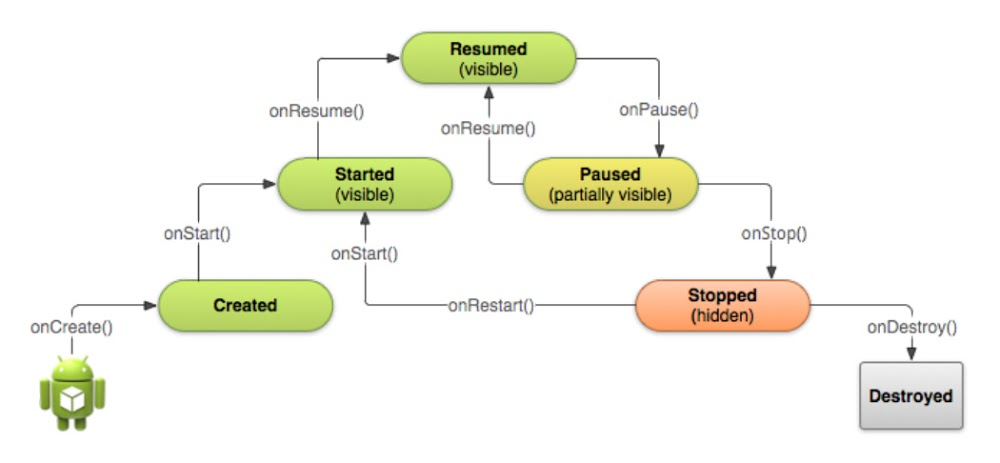
\includegraphics[width=0.8\columnwidth]{Figures/2/lifecycle}
% 		\caption{วัฏจักรของแอคทิวิตี้บนระบบปฏิบัติการแอนดรอยด์}{ที่มา : https://www.dev2qa.com/android-activity-lifecycle-example/}
% 		\label{Fig:lifecycle}
% 	\end{figure}
% 	จากรูปที่ \ref{Fig:lifecycle} แสดงวัฏจักรของแอคทิวิตี้ในรูปแบบโครงสร้างพีระมิดโดยแสดงให้เห็นว่า Method ที่เรียกใช้
% 	งานอัตโมัติ (Callback Method) ได้แก่ onCreate(), onStart(), onResume() และ onRestart() จะขยับแอคทิวิตี้ขึ้นไปด้านบนสุดที่ Resumed Method
% 	และมี Method ได้แก่ onPause(), onStop() และ onDestroy() ที่จะขยับแอคทิวิตี้ลงมาด้านล่าง แอคทิวิตี้ยังสามารถกลับไปทำงานที่ตำแหน่ง Resumed Method จากตำแหน่ง Paused และ Stopped ได้อีกด้วย
	
% 	ในบางครั้งไม่จำเป็นต้องเรียกใช้งาน Callback Method ทั้งหมดเสมอไปขึ้นกับความซับซ้อนของแอคทิวิตี้ อย่างไรก็ตามเป็นสิ่งสำคัญที่นักพัฒนาควรทำความเข้าใจแต่ละ Method เพื่อให้มั่นใจได้ว่าแอปพลิเคชันของที่ได้พัฒนาตอบสนองเป็นไปตามที่ผู้ใช้คาดหวัง ดังนั้น ในการใช้งาน Callback Method
% 	ที่ถูกวิธีก็จะช่วยให้แอปพลิเคชันทำงานได้เป็นอย่างดี ดังนี้
% 	\begin{itemize}
% 		\item ไม่หยุดการทำงานหรือค้าง กรณีมีสายโทรเข้าหรือมีการสลับไปใช้งานแอปพลิเคชันอื่น 
% 		\item ไม่ใช้ทรัพยากรที่มีค่าของระบบอย่างสูญเปล่า ถ้าไม่มีการใช้งานแอคทิวิตี้ใดๆ 
% 		\item ไม่กระทบต่อกระบวนการในขั้นตอนการใช้งานของผู้ใช้กรณีออกจากแอปพลิเคชันแล้วกลับเข้ามาใช้งานอีกครั้ง 
% 		\item ไม่หยุดการทำงานหรือระบบค้างที่กระทบการใช้งานของผู้ใช้กรณีมีการหมุนหน้าจอแนวนอนและแนวตั้งสลับกัน
% 	\end{itemize}
	
% 	เหตุการณ์ที่แอคทิวิตี้มีการเปลี่ยน Method ต่าง ๆ ตามแสดงในรูปที่  \ref{Fig:lifecycle}
% 	แต่มีอยู่ 3 Method เท่านั้นที่แอคทิวิตี้จะยังคงอยู่คงที่ในช่วงเวลาระยะเวลาหนึ่งไม่เปลี่ยนไป Method อื่นในทันที ได้แก่
% 		\begin{itemize}
% 		\item Resumed (แสดงอยู่ ทำงานอยู่) ใน Method นี้แอคทิวิตี้จะแสดงอยู่ด้านหน้าสุดและผู้ใช้กำลังใช้งานอยู่ บ่อยครั้งจะเรียกว่า Running Method
% 		\item Paused (แสดงหน้าจอบางส่วน ไม่ถูกบังสนิท) ใน Method นี้แอคทิวิตี้จะถูกบดบังด้วยแอคทิวิตี้อื่น เช่น แอคทิวิตี้อื่นที่อยู่ด้านหน้าสุดที่แสดงในลักษณะกึ่งโปรงใสหรือไม่ได้แสดงแบบเต็มหน้าจอ  แอคทิวิตี้ในสถานะนี้จะไม่สามารถรับค่าจากผู้ใช้และทำงานคำสั่งใด ๆ ได้
% 		\item Stopped (แสดงหน้าจอแบบ Background ผู้ใช้มองไม่เห็น) ใน Method นี้ แอคทิวิตี้จะถูกบดบังอย่างสมบูรณ์และผู้ใช้มองไม่เห็นโดยจะถูกย้ายไปอยู่ด้านหลังในขณะที่อยู่ใน Method นี้
% 		ค่า Activity Instance และตัวแปรทั้งหมดจะยังคงอยู่แต่จะไม่สามารถถูกเรียกมาใช้งานจากโค้ดใด ๆ ได้
% 		\end{itemize}
% 		ในขณะที่ Method อื่น เช่น Created และ Started จะแสดงชั่วคราวแล้วระบบก็จะเปลี่ยนไป Method อื่นในทันทีที่ Method ถูกเรียกใช้งานอัตโนมัติ นั่นคือ หลังจากที่ระบบเรียกใช้งาน onCreate() แล้วก็จะเรียกใช้งาน onStart()
% 		ทันทีและสุดท้ายตามด้วย onResumne()  ซึ่งก็จะเข้าสู่ Resumed Method ทั้งหมดก็คือวัฏจักรแอคทิวิตี้เบื้อต้น
		
% 	\subsection{การกำหนด Launcher Activity ในแอปพลิเคชัน}
% 	เมื่อผู้ใช้กดที่ Icon App จากหน้า Home Screen เพื่อใช้งาน ระบบก็จะเรียก onCreate() Method
% 	ขึ้นมาทำงานอัตโนมัติเพื่อที่จะเปิดใช้งานแอคทิวิตี้ที่ได้กำหนดให้เป็นแอคทิวิตี้หลัก ("launcher" หรือ "main" ) 
% 	ซึ่งก็จะเป็นแอคทิวิตี้ที่เป็นหน้าหลักที่ผู้ใช้จะเห็นเมื่อเข้ามาใช้งานแอปพลิเคชัน สามารถกำหนดได้ว่าแอคทิวิตี้ใดที่จะใช้เป็น Activity หลักโดยกำหนดค่าในไฟล์ AndroidManifest.xml
	
% 	แอคทิวิตี้หลักจะต้องกำหนด ค่าใน manifest ด้วย <intent-filter> 
% 		\begin{figure}[H]
% 			{\setstretch{1.0}\begin{lstlisting}
% <intent-filter>
% <action android:name="android.intent.action.MAIN" />
% <category android:name="android.intent.category.LAUNCHER" />
% </intent-filter>
% 					\end{lstlisting}}
% 					\caption{การกำหนด Launcher Activity ในแอปพลิเคชัน}
% 					\label{Fig:Launcher}
% 		\end{figure}
% โดยประกอบไปด้วย MAIN action และ LAUNCHER category ดังตัวอย่างดังนี้
% 				\begin{figure}[H]
% 					{\setstretch{1.0}\begin{lstlisting}
% <Activity android:name=".MainActivity" android:label="@string/app_name">
% <intent-filter>
% <action android:name="android.intent.action.MAIN" />
% <category android:name="android.intent.category.LAUNCHER" />
% </intent-filter>
% </Activity>
% 						\end{lstlisting}}
% 					\caption{การกำหนด Launcher Activity ในแอปพลิเคชัน}
% 					\label{Fig:category}
% 				\end{figure}
%    ใน Android Studio เมื่อสร้างโปรเจค (Project) ขึ้นมาจะมีการประกาศค่าและกำหนดให้มีการเรียกใช้งาน filter ในไฟล์ AndroidManifest.xml มาให้เรียบร้อยแล้ว ถ้าไม่ได้กำหนด MAIN action และ LAUNCHER category แล้ว App Icon ของจะไม่แสดงในหน้าหลักของลิสรายการแอปพลิเคชันบนหน้าจอสมาร์ทโฟนของผู้ใช้
% 	\subsection{การสร้าง Instance ใหม่}
% 	แอปพลิเคชันส่วนใหญ่จะประกอบไปด้วยแอคทิวิตี้หลายอันทำงานแตกต่างกันไป  ไม่ว่าจะเป็นแอคทิวิตี้หลักที่ถูกสร้างขึ้นเมื่อผู้ใช้คลิกที่ icon app หรือแอคทิวิตี้ต่าง ๆ ที่ถูกเรียกใช้งานโดยผู้ใช้ ทั้งหมดล้วนแล้วเป็นสิ่งที่ระบบสร้าง instance ใหม่ของแอคทิวิตี้โดยการเรียกใช้ผ่าน onCreate() Method ต้องใช้ onCreate() Method ในเหตุผลเพื่อเริ่มต้นแอปพลิเคชันซึ่งควรจะเกิดขึ้นเพียงครั้งเดียวตลอดหนึ่งวัฏจักรของแอคทิวิตี้เช่น ใช้ onCreate() กำหนดหน้าตาของแอปพลิเคชันหรือประกาศตัวแปรที่จะถูกใช้งานในคลาส (Class) เป็นต้น ตัวอย่างการใช้งาน onCreate() Method ตามตัวอย่างรูปที่ \ref{Fig:onCreate} แสดง code เพื่อให้เห็นการตั้งค่าเบื่องต้นเช่น การกำหนด User interface(โดยใช้ XML layout ไฟล์) การประกาศตัวแปรต่าง ๆ การตั้งค่ากำหนดเงื่อนไข UI 
% 					\begin{figure}[H]
% 						{\setstretch{1.0}\begin{lstlisting}
% TextView mTextView; // การประกาศตัวแปรจำหรับ text view ใน layout

% @Override
% public void onCreate(Bundle savedInstanceMethod) {
% 	super.onCreate(savedInstanceMethod);

% // การกำหนด user interface (โดยใช้ XML layout ไฟล์) 
% // ไฟล์ layout ใน project จะอยู่ที่  res/layout/main_Activity.xml 
% 	setContentView(R.layout.main_Activity);

% // กำหนดค่าให้กับ TextView ดังนั้นสามารถเรียกใช้งานผ่านชื่อตัวแปรได้ภายหลัง
% 	mTextView = (TextView) findViewById(R.id.text_message);

% // ตั้งค่าสำหรับกำหนดเงื่อนไข UI 
% // ตรวจสอบเพื่อยืนยันว่ากำลังใช้งานบน android  Honeycomb   
% // หรือสูงกว่า เพื่อเรียกใช้ ActionBar API  
% 	if (Build.VERSION.SDK_INT >= Build.VERSION_CODES.HONEYCOMB) {
% 		// กำหนดให้ icon ใน action bar ไม่ทำงานคล้ายปุ่ม Home  
% 		ActionBar actionBar = getActionBar();
% 		actionBar.setHomeButtonEnabled(false);
% 	}
% }
% 							\end{lstlisting}}
% 						\caption{การใช้งาน onCreate()}
% 						\label{Fig:onCreate}
% 					\end{figure}
% 		เมื่อ onCreate() ทำงานเสร็จระบบจะเรียก onStart() และ onResume() memthod มาทำงานต่อในทันที แอคทิวิตี้จะไม่อยู่ใน Created Method หรือ Started Method ในทางเทคนิคแอคทิวิตี้จะแสดงขึ้นมาทันทีที่ onStart() ถูกเรียกใช้งานแต่ onResume() จะแสดงตามมาติด ๆ ในทันทีและจะอยู่ใน Resumed Method จนกว่าจะมีการเปลี่ยนแปลงบางอย่างเกิดขึ้นเช่น มีสายโทรเข้าหรือผู้ใช้เปิดไปแอคทิวิตี้อื่นหรือปิดหน้าจอลง
		
% 		 โครงสร้างของวัฏจักรแอคทิวิตี้ที่เน้นไปที่ 3 Method หลักที่ระบบเรียกใช้อัตโนมัติตามลำดับ เมื่อมีการสร้าง Instance
% 		 ของแอคทิวิตี้ขึ้นมาใหม่ ได้แก่ onCreate(), onStart() และ onResume() เมื่อลำดับการทำงานเสร็จสิ้นลงแอคทิวิตี้จะ
% 		 มาอยู่ที่ Resumed Method ซึ่งผู้ใช้ใช้งานอยู่จนกว่าจะเปลี่ยนไปเรียกใช้งานแอคทิวิตี้อื่นขึ้นมา
		 
% 	\subsection{การสิ้นสุดการทำงานของแอคทิวิตี้ (Destroy Activity)}
% 	ในขณะที่วัฏจักรของแอคทิวิตี้มี Method แรกคือ onCreate() และ Method สุดท้ายคือ onDestroy()
% 	ระบบจะเรียก Method นี้ในแอคทิวิตี้เป็นสัญญาณว่า Activity instance นี้จะถูกลบบออกอย่างสมบูรณ์จากหน่วยความจำของระบบ (System memory)
	
% 	แอปพลิเคชันส่วนใหญ่ไม่จำเป็นต้องกำหนด Method นี้เพราะ local class ถูกทำลายไปพร้อมกับแอคทิวิตี้และแทบจะถูกลบไปอย่างสมบูร์ในระหว่างเรียกใช้งาน onPause() และ onStop() อย่างไรก็ตามถ้าแอคทิวิตี้ของมีการกำหนดให้มีการทำงานแบบ background (ทำงานอยู่เบื้องหลัง) ในขั้นตอน onCreate() ด้วยแล้วหรือมีการใช้งานทรัพยากรของระบบเป็นระยะเวลานานเป็นเหตุให้ความจำถูกใช้งานจำนวนมาก หากไม่ทำการปิดการใช้งาน จึงควรอย่างยิ่งที่จะเรียกใช้งาน Method onDestroy() เพื่อคืนค่าหน่วยความจำให้ระบบ
% 						\begin{figure}[H]
% 							{\setstretch{1.0}\begin{lstlisting}
% @Override
% public void onDestroy() {
% 	super.onDestroy();  // เรียกใช้งาน superclass ทุกครั้งเสมอ

% // หยุดการติดตามหรือตรวจจับ Method ของ Activity 
% 	android.os.Debug.stopMethodTracing();
% }
% 								\end{lstlisting}}
% 							\caption{การใช้งาน onDestroy()}
% 							\label{Fig:onDestroy}
% 						\end{figure}
% 	ระบบจะเรียกใช้งาน onDestroy() หลังจากเรียกใช้งาน onPause() และ onStop() แล้วในทุกเหตุการณ์ ยกเว้นกรณีมีการกำหนดให้เรียกใช้ finish() ภายใน onCreate() Method ในกรณีเช่น Activity หยุดชั่วคราวเพื่อทำการเรียกใช้งานแอคทิวิตี้อื่นข้ามาแล้วทำการกำหนดให้มีการเรียกใช้งาน finish() ที่กำหนดใน onCreate() Method เพื่อทำลายแอคทิวิตี้ในกรณีนี้ระบบจะทำการเรียก onDestroy() ทันทีโดยไม่ผ่าน Callback Method อื่นเช่น ไม่ผ่าน onPause() หรือ onStop() แบบนี้เป็นต้น
\newpage

\section{ความรู้พื้นฐาน Java}
Java \cite{java} เป็นภาษาเขียนโปรแกรมเพื่อวัตถุประสงค์ทั่วไป โดยสามารถทำงานได้พร้อมกัน เป็นภาษาที่สร้างมาจากคลาส และสนับสนุนการเขียนโปรแกรมแบบออบเจ็คอย่างสมบูรณ์ และถูกออกแบบมาให้พร้อมสำหรับการใช้งานมากที่สุด ซึ่งมีเมธอดและคลาสต่าง ๆ อำนวยความสะดวกให้ใช้มากมาย โดยภาษา Java นั้นมีความตั้งใจว่าจะทำให้นักพัฒนาออกแบบและพัฒนาโปรแกรมน้อยลง นั่นคือการเขียนเพียงครั้งเดียว แต่นำไปใช้งานได้ทุกที่หรือทุกแพลตฟอร์ม

แอปพลิเคชันของภาษา Java นั้นโดยปกติแล้วจะคอมไพล์เป็น bytecode ที่สามารถรันได้ใน Java virtual machine (JVM) ขึ้นกับสถาปัตยกรรมของคอมพิวเตอร์นั้นๆ และใน ปี 2016 ภาษา Java เป็นภาษาที่ได้รับความนิยมและใช้มากที่สุดในโลก โดยเฉพาะการใช้พัฒนาเว็บแอปพลิเคชัน

	\subsection{ประวัติความเป็นมาของภาษา Java}
	James Gosling Mike Sheridan และ Patrick Naughton ได้เริ่มก่อตั้งโปรเจ็คภาษา Java เมื่อปี 1991 โดยในตอนแรกถูกพัฒนาสำหรับทีวีที่สามารถมีปฎิสัมพันธ์ได้ เช่น เล่นเกมในทีวี แต่ประสบปัญหาในการที่จะใช้งานกับสายเคเบิลของทีวีดิจิตอล ในตอนแรกภาษา Java ใช้ชื่อว่า Oak เพราะว่ามีต้นโอ็คยื่นออกไปยังออฟฟิศของ Gosling ต่อมาใช้ชื่อว่า Green และในตอนท้ายใช้ชื่อว่า Java มีที่มาจากกาแฟ Java 
	
	ภาษาได้รับการออกแบบให้มีรูปแบบทางภาษาเหมือนภาษา C และ C++ ซึ่งทำให้โปรแกรมเมอร์ส่วนมากนั้นคุ้นเคยกับมันได้ดีขึ้น และ Sun Microsystems เผยแพร่ Java 1.0 ในปี 1995 โดยมีคำกล่าวว่า "Write Once, Run Anywhere" (WORA)  เขียนเพียงครั้งเดียวและสามารถนำไปใช้งานได้บนทุกแพลตฟอร์ม

	\section{ความรู้พื้นฐาน Python}
	Python \cite{py} เป็นภาษาเขียนโปรแกรมระดับสูงที่ใช้กันอย่างกว้างขวางในการเขียนโปรแกรมสำหรับวัตถุประสงค์ทั่วไป 
	ภาษา Python นั้นสร้างโดย Guido van Rossum และถูกเผยแพร่ครั้งแรกในปี 1991 Python 
	นั้นเป็นภาษาแบบ interprete ที่ถูกออกแบบโดยมีปรัญชาที่จะทำให้โค้ดอ่านได้ง่ายขึ้น
	 และโครงสร้างของภาษานั้นจะทำให้โปรแกรมเมอร์สามารถเข้าใจแนวคิดการเขียนโค้ดโดยใช้บรรทัดที่น้อยลงกว่าภาษาอย่าง 
	 C++ และ Java ซึ่งภาษานั้นถูกกำหนดให้มีโครงสร้างที่ตั้งใจให้การเขียนโค้ดเข้าใจง่ายทั้งในโปรแกรมเล็กไปจนถึงโปรแกรมขนาดใหญ่
	 
	\subsection{ประวัติความเป็นมาของภาษา Python}
	Python กำเนิดขึ้นตั้งแต่ 1980 
	และเริ่มต้นใช้งานกันช่วงธันวาคม 1989 โดยนาย
	Gudio Van Rossum
	 ภายใต้ Centrum Wiskunde and Informatica (CWI) ที่ Netherlands\cite{bpy}	
% 	\subsection{Java Compiler}
% 	ในการเขียนโปรแกรมในภาษา Java ต้องการ Java Compiler เพื่อทำการแปลงโค้ดของโปรแกรมที่เขียนเป็น bytecode เพื่อนนำไปรันในแต่ละแพลตฟอร์มต่อไป โดยเรียกว่า Java Platform (JDK) ซึ่งประกอบไปด้วยคอมไพล์เลอร์ ในการแปลงโค้ดภาษา Java ให้เป็น Bytecode และ Java virtual machine (JVM) สำหรับรันโปรแกรมของภาษา Java ในแต่ละแพลตฟอร์ม สำหรับในบทเรียนนี้จะใช้ IDE ในการพัฒนาเพื่อความสะดวกและรวดเร็ว
	
% 	\subsection{โครงสร้างของภาษา Java}

%   \begin{figure}[H]
%     \begin{minted}[frame=lines,framesep=2mm,baselinestretch=1.15,fontsize=\footnotesize,linenos]{java}
%     public class ClassName {
%       public static void main(String[] args) {
%         System.out.println("Hello สวัสดี");
%       }
%     }
%     \end{minted}
%     \caption{ตัวอย่างโปรแกรมภาษา Java ด้วย minted}
%     \label{Fig:JavaClassMinted}
%   \end{figure}
  
%   รูปที่ \ref{Fig:JavaClassMinted} แสดงให้เห็นผลลัพธ์ของการใช้ minted เพื่อแสดงคำสั่งในเอกสาร Latex

% 	\begin{itemize}
% 		\item Package เป็นกลุ่มของคลาสหรือไลบรารี่มาตรฐานของภาษา Java ที่มีฟังก์ชันต่าง ๆ ให้ใช้มากมาย
% 		\item Class ในส่วนของการประกาศคลาส จะต้องประกาศคลาสให้ชื่อตรงกับไฟล์เสมอ นอกจาก Inner คลาสที่อยู่ในคลาสเดียวกัน โดยชื่อคลาสนั้นควรจะขึ้นต้นด้วยตัวใหญ่และถ้ามีหลายคำให้ใช้ตัวพิมพ์ใหญ่แบ่ง ดังตัวอย่างในรูปที่ \ref{Fig:ClassName}
% 				\begin{figure}[H]
% 					{\setstretch{1.0}\begin{lstlisting}
% public class ClassName {
% ...
% }
% 						\end{lstlisting}}
% 					\caption{การงประกาศคลาสในภาษา Java}
% 					\label{Fig:ClassName}
% 				\end{figure}
% 			\item Method หลังจากคลาสสร้างแล้ว จะเป็นประกาศเมธอดภายในคลาส โดยในการที่จะรันโปรแกรมได้จะต้องมีเมธอดที่ชื่อว่า Main ดังตัวอย่างในโปรแกรมด้านบน มันเป็นที่แรกที่โปรแกรมจะเริ่มทำงาน \ref{Fig:ClassName}
% 			\begin{figure}[H]
% 				{\setstretch{1.0}\begin{lstlisting}
% public static void main (String[] args) {
% ...
% }
% 					\end{lstlisting}}
% 				\caption{การงประกาศเมธอด main ในภาษา Java}
% 				\label{Fig:main}
% 			\end{figure}
% 			\item Methodments เป็นคำสั่งของโปรแกรมเพื่อให้โปรแกรมทำงานตามต้องการ เช่น System.out.println("Hello World!"); เป็นการแสดงผลข้อความออกทางหน้าจอ โดยปกติโปรแกรมมักจะมีหลายคำสั่ง
% 			\item Semicolon ทุกคำสั่งการทำงานของโปรแกรมในภาษา Java จะจบด้วยเครื่องหมาย Semicolon (;) นั่นหมายความว่าสามารถเขียนโปรแกรมแบบไหนก็ได้ โดยคอมไพเลอร์จะทราบอัตโนมัติว่าสิ้นสุดคำสั่งที่ไหน
% 			\item ในภาษา Java สามารถใช้ White space ได้อย่างอิสระตามที่ต้องการ โดย White space จะประกอบไปด้วย Space bar Tab และ Enter (return) เพราะว่าคอมไพเลอร์ตรวจการสิ้นสุดของคำสั่งด้วย ; ใช้ while space ทำให้โค้ดอ่านเข้าใจง่าย และเป็นระเบียบ
% 			\item Literals คือค่าของข้อมูลใดๆ ที่กำหนดให้กับตัวแปรได้ เรียกว่า Constant Literals ทุกค่าที่เป็นไปได้ เช่น "MarcusCode" เป็น String Literals 10 เป็น Integer Literals หรือ true เป็น Boolean Literals โดย Literals เป็นได้แค่ Primitive data type เท่านั้น ตัวอย่างการกำหนดค่าหรือ Literals ให้กับตัวแปร
% 			\item Expression เป็นการกระทำระหว่างตัวแปรกับตัวดำเนินการเพื่อให้ได้ผลลัพธ์ใหม่ เช่น 4 + 3 เป็น expression ของการบวกเลขและได้ได้ผลลัพธ์เท่ากับ 7 หรือ 1 == 1 เป็น expression ของการเปรียบเทียบระหว่างค่าสองค่าว่าเท่ากันหรือไม่ และได้ผลลัพธืเป็น true
% 			\item Keyword คือคำที่สงวนไว้ในภาษา Java นั่นหมายความว่าไม่สามารถนำคำเหล่านี้ไปประกาศเป็นชื่อตัวแปร เมธอด หรือว่าคลาสได้ เพราะว่า Keyword ถูกใช้โดยคอมไพเลอร์เพื่อให้มันทำงานได้สมบูรณ์
% 		\end{itemize}
	

	 
	 \section{ความรู้พื้นฐาน Tensorflow Lite}
	 Tensorflow Lite คือ Library ที่ถูก optimize จาก Tensorflow ทำให้มีขนาดเล็กลงทำให้สามารถทำงานบนอุปกรณ์พกพาได้ ใช้สำหรับพัฒนา Machine Learning Deep Learning และ Neural Network ได้รับการพัฒนาโดยบริษัท Google 
	 ได้ทำการเปิดตัวในงาน I/O ปี 2017 รองรับระบบปฏิบัติการ Android และ IOS ลำดับชั้นในการเรียกใช้ TensorFlow Lite แอพจะเรียกใช้งานผ่านเอนจิน TensorFlow Lite ที่ฝังมาในตัวแอปพลิเคชัน จากนั้น TensorFlow Lite จะเรียกใช้ฟีเจอร์ Android Neural Networks (Android NN) ของ ระบบปฏิบัติการ ที่เริ่มมีการใส่เข้ามาใน Android 8.1
	ลำดับสุดท้าย Android Neural Network จะเรียกใช้ตัวเร่งการประมวลผลที่ระดับฮาร์ดแวร์ 
%			\begin{figure}[H]
%				\centering
%				
\includegraphics[width=0.4\columnwidth]{Figures/2/vuelogo}
%				\caption{ตราสัญลักษณ์ของวิวเจเอส}{ที่มา : https://seeklogo.com/vector-logo/274070/vue-js}
%				\label{Fig:oop}
%			\end{figure}
%		\subsection{ภาพรวมของ Vue.js}
		
	
    \section{ความรู้พื้นฐาน Image Processing}
		Image Processing \cite{imgp} หรือ การประมวลผลภาพดิจิทัล เป็นการแปลงข้อมูลรูปที่เป็นสัญญาณแอนะล็อกให้อยู่ในรูปของสัญญาณดิจิทัล เพื่อใช้ในการประมวลผลผ่านทางคอมพิวเตอร์ได้ และ ยังนำมาใช้ในการลดปัญหาของภาพเช่น ลดสัญญาณรบกวนภายในภาพเป็นต้น

		ในการแปลงภาพให้เป็นสัญญาณดิจิทัลนั้น ระบบจะนำรูปที่รับเข้ามาไปคำนวณ โดยกระบวนการSampling และ Quantization และส่งข้อมูลออกมาในรูปแบบดิจิทัล คอมพิวเตอร์จะเก็บข้อมูลภาพลงหน่วยความจำ โดยการจองหน่วยความจำภายในเครื่องในรูปแบบของอาร์เรย์ โดยค่าในแต่ละช่องของ อาร์เรย์แสดงถึงคุณสมบัติต่างๆของรูปที่จุด พิกเซล นั้นๆ และตำแหน่งของช่อง อาร์เรย์ก็เป็นตัวกำหนดตำแหน่งของจุด พิกเซล ภายในภาพด้วย
		
		\begin{figure}[H]
			\centering
			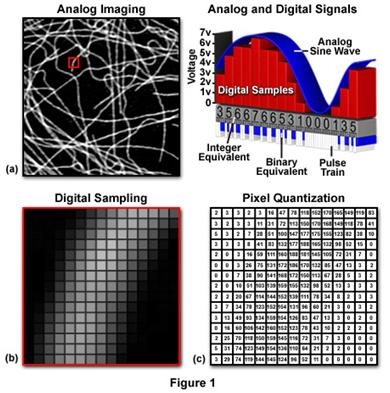
\includegraphics[width=0.8\textwidth]{Figures/2/1.jpg}
			\caption{การแปลงภาพแอนะล็อกให้เป็นภาพดิจิทัล}{ที่มา : https://nextsoftwares.wordpress.com/2014/05/22/}
			\label{Fig:Studentloan1}
		\end{figure}
		ภาพดิจิทัลที่ได้จะมีรูปแบบการเก็บเป็นเมทริกซ์ ซึ่งจะมีการจัดเก็บภาพแต่ละชนิดต่างกัน ขึ้นอยู่กับระบบสีของภาพดังกล่าว โดยแบ่งชนิดของภาพได้ดังนี้
		   \begin{itemize}
			   	\item   Binary imageหรือ ภาพขาว-ดำ เป็นรูปที่ใช้เนื้อที่เพียง 1 บิต ต่อ พิกเซล โดยค่าสีจะมีแค่สองค่าคือ 0 หรือสีดำ และ 1 หรือสีขาว
				 
					 \begin{figure}[H]
						\centering
						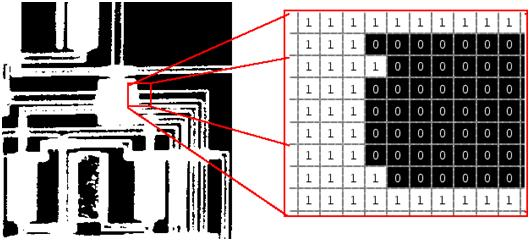
\includegraphics[width=0.8\textwidth]{Figures/2/2.jpg}
						\caption{ภาพแบบ Binary หรือ ภาพขาว-ดำ}{ที่มา : https://nextsoftwares.wordpress.com/2014/05/22/}
						\label{Fig:Studentloan1}
					\end{figure}

						\item  Grayscale Image เป็นรูปที่เก็บโดยใช้รูปแบบของอาร์เรย์ 2 มิติ โดยค่าที่เก็บจะมีค่าอยู่ในช่วงๆหนึ่ง ซึ่งระดับของสีขึ้นอยู่กับขนาดของบิตที่ใช้เก็บค่าสี

						\begin{figure}[H]
							\centering
							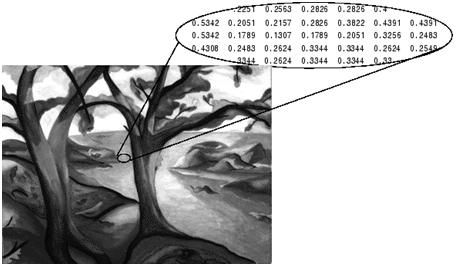
\includegraphics[width=0.8\textwidth]{Figures/2/3.jpg}
							\caption{ภาพแบบ Grayscale}{ที่มา : https://nextsoftwares.wordpress.com/2014/05/22/}
							\label{Fig:Studentloan1}
						\end{figure}
								\item RGB Image หรือ Truecolor Image เป็นรูปที่เก็บโดยใช้อาร์เรย์ 3 มิติ ขนาด m x n x 3 โดยที่ m คือความยาว และ n คือความกว้างของภาพในหน่วยพิกเซล ส่วนมิติสุดท้ายนั้น ในแต่ละมิติจะเก็บค่าสีแยกกัน คือสีแดง(Red) สีเขียว(Green) และสีน้ำเงิน(Blue)
							\begin{figure}[H]
									\centering
									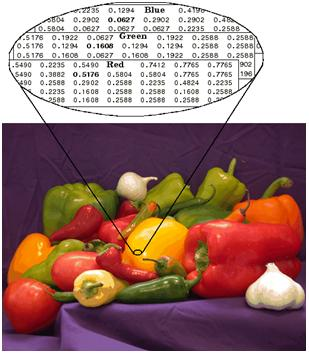
\includegraphics[width=0.4\textwidth]{Figures/2/4.jpg}
									\caption{ภาพแบบ RGB}{ที่มา : https://nextsoftwares.wordpress.com/2014/05/22/}
									\label{Fig:Studentloan1}
								\end{figure}
					
									\item  Indexed Image เป็นรูปที่มีรูปแบบการเก็บแบบ indexed คือ ภาพประเภทนี้จะเก็บค่าสีเป็น indexed และในแต่ละช่องอาร์เรย์ จะเก็บตำแหน่งของสีใน indexed นั้นๆไว้

									\begin{figure}[H]
										\centering
										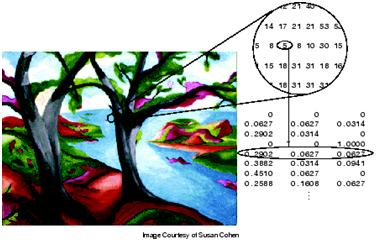
\includegraphics[width=0.8\textwidth]{Figures/2/6.jpg}
										\caption{ภาพNeural Network โครงข่ายประสาทเทียม}{ที่มา : https://nextsoftwares.wordpress.com/2014/05/22/}
										\label{Fig:Studentloan1}
									\end{figure}

								\end{itemize}

								\section{ความรู้พื้นฐาน ปัญญาประดิษฐ์}
								ปัญญาประดิษฐ์ \cite{AI} หรือ Artificial Intelligence  เป็นศาสตร์แขนงหนึ่งของวิทยาศาสตร์คอมพิวเตอร์ ที่เกี่ยวข้องกับวิธีการทำให้คอมพิวเตอร์มีความสามารถคล้ายมนุษย์หรือเลียนแบบพฤติกรรมมนุษย์ คือโปรแกรม Software (ซอฟแวร์) ต่าง ๆ ที่ใช้กับคอมพิวเตอร์ โดยเฉพาะความสามารถในการคิดเองได้ หรือมีปัญญานั่นเอง ปัญญานี้มนุษย์เป็นผู้สร้างให้คอมพิวเตอร์ จึงเรียกว่า ปัญญาประดิษฐ์ 
	 คำนิยาม AI ตามความสามารถที่มนุษย์ต้องการแบ่งได้ 4 กลุ่ม ดังนี้
	 \begin{itemize}
		\item  การกระทำคล้ายมนุษย์ Acting Humanly การสร้างเครื่องจักรที่ทำงาน, สามารสื่อสารได้ด้วยภาษาที่มนุษย์ใช้ เช่น ภาษาไทย ภาษาอังกฤษ เช่น การแปลงข้อความเป็นคำพูด และ การแปลงคำพูดเป็นข้อความ, 
		มีประสาทรับสัมผัสคล้ายมนุษย์ เช่น คอมพิวเตอร์รับภาพได้โดยอุปกรณ์รับสัมผัส แล้วนำภาพไปประมวลผล,เคลื่อนไหวได้คล้ายมนุษย์ เช่น หุ่นยนต์ช่วยงานต่าง ๆ อย่างการ ดูดฝุ่น เคลื่อนย้ายสิ่งของ และเรียนรู้ได้ โดยสามารถตรวจจับรูปแบบการเกิดของเหตุการณ์ใด ๆ แล้วปรับตัวสู่สิ่งแวดล้อมที่เปลี่ยนไปได้
		\item  การคิดคล้ายมนุษย์ Thinking Humanly  กลไกของกิจกรรมที่เกี่ยวข้องกับความคิดมนุษย์ เช่น การตัดสินใจ การแก้ปัญหา การเรียนรู้
		\item  คิดอย่างมีเหตุผล Thinking rationally การศึกษาความสามารถในด้านสติปัญญาโดยการใช้โมเดลการคำนวณ, การศึกษาวิธีการคำนวณที่สามารถรับรู้ ใช้เหตุผล และกระทำ และใช้หลักตรรกศาสตร์ในการคิดหาคำตอบอย่างมีเหตุผล เช่น ระบบผู้เชี่ยวชาญ
		\item กระทำอย่างมีเหตุผล Acting rationally การศึกษาเพื่อออกแบบโปรแกรมที่มีความสามารถในการกระทำ หรือเป็นตัวแทนในระบบอัตโนมัติต่าง ๆ ที่มีปัญญา, พฤติกรรมที่แสดงปัญญาในสิ่งที่มนุษย์สร้างขึ้น และการเพื่อบรรลุเป้าหมายที่ได้ตั้งไว้ เช่น โปรแกรมเล่นเกมหมากรุก ที่จะทำให้คู่ต่อสู้แพ้ให้ได้
		
	\end{itemize}
	% \section{ความรู้พื้นฐาน โครงข่ายประสาทเทียม }
	% โครงข่ายประสาทเทียม  \cite{vuejs} หรือ Artificial Neural Networks คือโมเดลทางคณิตศาสตร์ สำหรับประมวลผลสารสนเทศด้วยการคำนวณแบบคอนเนคชันนิสต์ (Connectionist) เพื่อจำลองการทำงานของเครือข่ายประสาทในสมองมนุษย์ ด้วยวัตถุประสงค์ที่จะสร้างเครื่องมือซึ่งมีความสามารถในการเรียนรู้การจดจำรูปแบบ(Pattern Recognition) และการสร้างความรู้ใหม่ (Knowledge Extraction)
	% เช่นเดียวกับความสามารถที่มีในสมองมนุษย์ สำหรับในคอมพิวเตอร์ Neurons ประกอบด้วย input และ output เหมือนกัน โดยจำลองให้ input แต่ละอันมี weight เป็นตัวกำหนดน้ำหนักของ input โดย neuron แต่ละหน่วยจะมีค่า threshold เป็นตัวกำหนดว่าน้ำหนักรวมของ input ต้องมากขนาดไหนจึงจะสามารถส่ง output ไปยัง neurons ตัวอื่นได้ เมื่อนำ neuron แต่ละหน่วยมาต่อกันให้ทำงานร่วมกันการทำงานนี้ในทางตรรกแล้วก็จะเหมือนกับปฏิกิริยาเคมีที่เกิดในสมอง		

	% \begin{figure}[H]
	% 	\centering
	% 	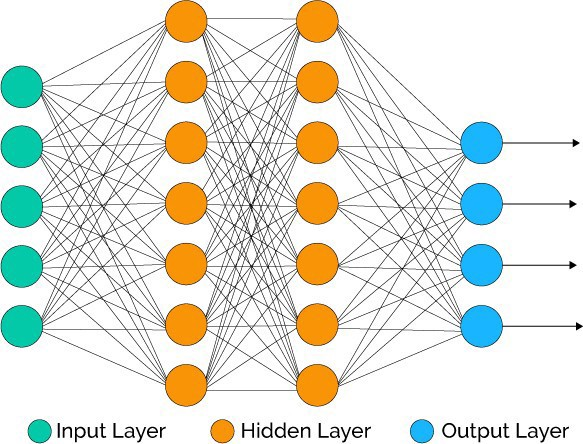
\includegraphics[width=0.4\textwidth]{Figures/2/9.jpeg}
	% 	\caption{Neural Network โครงข่ายประสาทเทียม}{ที่มา :  https://towardsdatascience.com/machine-learning-fundamentals-ii-neural-networks-f1e7b2cb3eef}
	% 	\label{Fig:Studentloan1}
	% \end{figure}
	% \subsection{การเรียนรู้ของ โครงข่ายประสาทเทียม}
	% 		การเรียนรู้ของโครงข่ายประสาทเทียมแบ่งได้ 2 ประเภทดังนี้
	% 		\begin{itemize}
	% 			\item Supervised Learning การเรียนแบบมีการสอน
	% 			เป็นการเรียนแบบที่มีการตรวจคำตอบเพื่อให้โครงข่ายประสาทเทียมปรับตัว ชุดข้อมูลที่ใช้สอนโครงข่ายประสาทเทียมจะมีคำตอบไว้คอยตรวจดูว่าโครงข่ายประสาทเทียมให้คำตอบที่ถูกหรือไม่ ถ้าตอบไม่ถูก โครงข่ายประสาทเทียมก็จะปรับตัวเองเพื่อให้ได้คำตอบที่ดีขึ้น 
				
	% 			\begin{figure}[H]
	% 				\centering
	% 				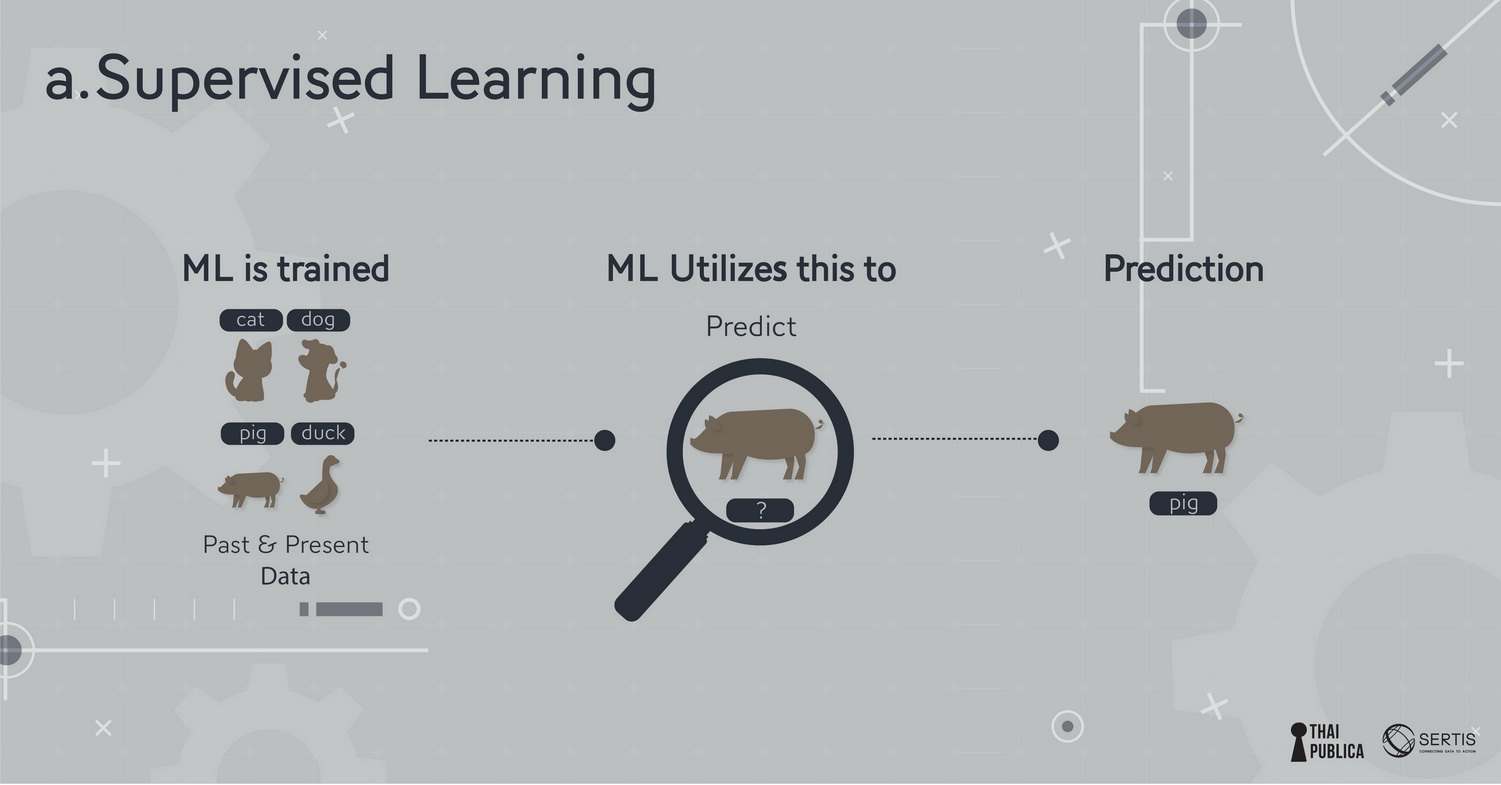
\includegraphics[width=0.8\textwidth]{Figures/2/7.jpg}
	% 				\caption{โมเดลที่ถูกสอนแบบ supervised learning}{ที่มา : https://thaipublica.org/2017/07/data-driven-society12/}
	% 				\label{Fig:Studentloan1}
	% 			\end{figure}
				
	% 			\item  Unsupervised Learning การเรียนแบบไม่มีการสอน
	% 			เป็นการเรียนแบบไม่มีผู้แนะนำ ไม่มีการตรวจคำตอบว่าถูกหรือผิด โครงข่ายประสาทเทียมจะจัดเรียงโครงสร้างด้วยตัวเองตามลักษณะของข้อมูล ผลลัพธ์ที่ได้ โครงข่ายประสาทเทียมจะสามารถจัดหมวดหมู่ของข้อมูลได้ 
	% 			\begin{figure}[H]
	% 				\centering
	% 				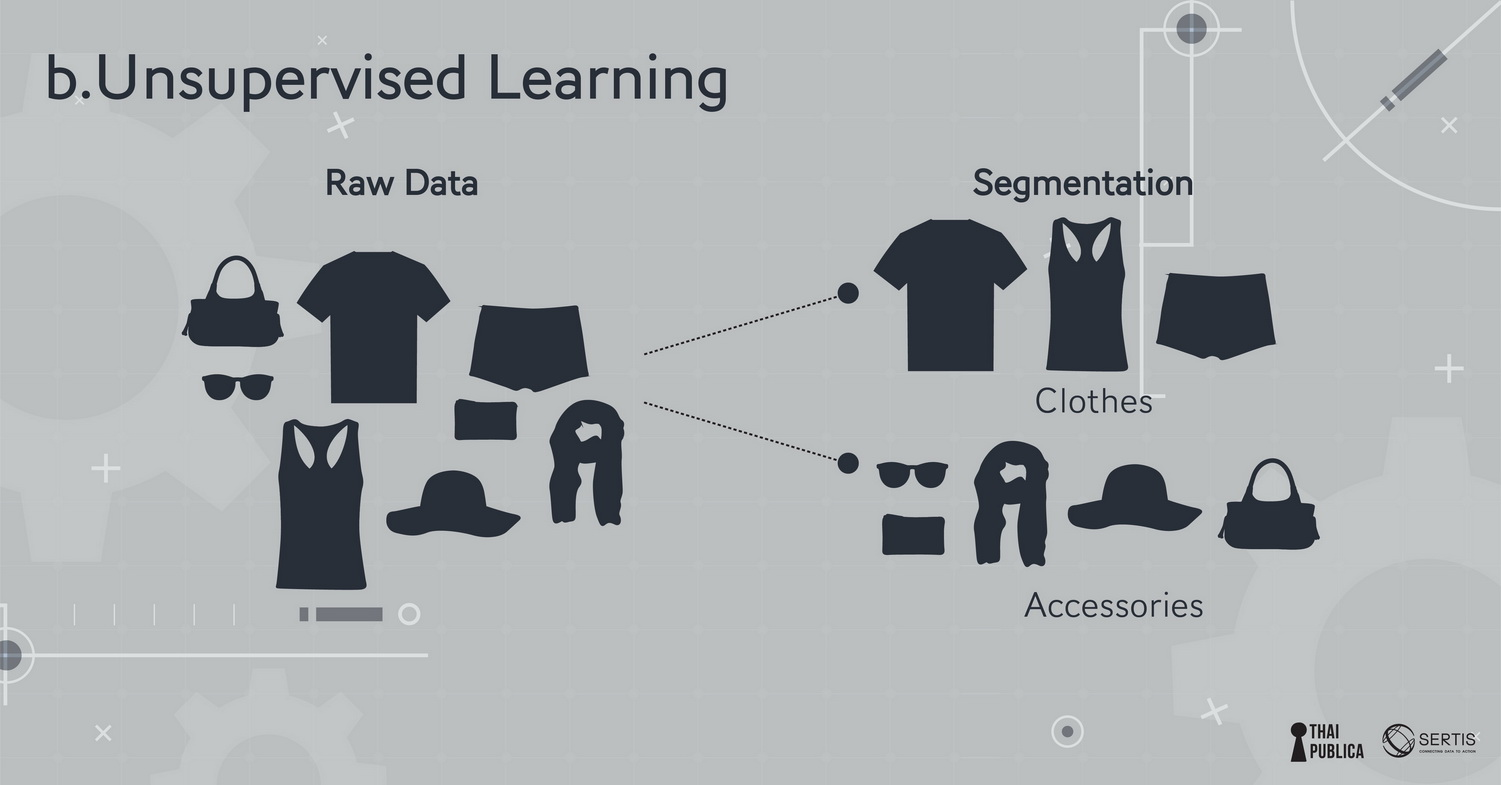
\includegraphics[width=0.8\textwidth]{Figures/2/8.jpg}
	% 				\caption{โมเดลที่ถูกสอนแบบ unsupervised learning}{ที่มา : https://thaipublica.org/2017/07/data-driven-society12/}
	% 				\label{Fig:Studentloan1}
	% 			\end{figure}
	% 		\end{itemize}


% 			\section{ความรู้พื้นฐานเกี่ยวกับการเรียนรู้ของเครื่อง (Machine Learning) }
% 			Firebase  \cite{vuejs} คือ Platform ที่รวบรวมเครื่องมือต่าง ๆ สำหรับการจัดการในส่วนของ Backend หรือ Server side ซึ่งทำให้สามารถ Build Mobile Application ได้อย่างมีประสิทธิภาพ และยังลดเวลาและค่าใช้จ่ายของการทำ Server side หรือการวิเคราะห์ข้อมูล โดยมีทั้งเครื่องมือที่ฟรี และเครื่องมีที่มีค่าใช้จ่าย 
% เครื่องมือ Firebase มีดังนี้
% 			\begin{enumerate}
% 				\item  Cloud Firestore คือ เครื่องมือ Database ที่เป็นลักษณะเป็น NoSQL โดยนำข้อดีของ Realtime Database ของ Firebase มาพัฒนาต่อ
% 				\item  Authentication  คือ  เครื่องมือ  Authentication ซึ่งคลอบคลุมทั้ง email-password, phone ไปจนถึง facebook, twitter, github สำหรับการ Login 
% 				\item  Hosting คือ hosting สำหรับ single-page web app, landing page website ซึ่งจัดการการ Deploy  และมีการติดตั้ง SSL ให้กับในส่วน Custom Domain  
% 				\item  Crashlytics ช่วยจัดการ Issue ต่าง ๆ และสามารถตรวจจับ Crash ได้ว่าเกิดขึ้นที่การทำงานไหนใน Mobile App 
% 				\item  Performance Monitoring  โดยผู้พัฒนาสามารถดู Performance ของ Code และ Network
% 			\end{enumerate}
			
\section{ความรู้พื้นฐานเกี่ยวกับการเรียนรู้เชิงลึก (Deep Learning)}
การเรียนรู้เชิงลึก \cite{deeplearning} คือโครงข่ายใยประสาทเสมือน (ANN: Artificial Neuron Networks) โดยการเรียนรู้เชิงลึกและโครงข่ายใยประสาทเสมือนเป็นอัลกอริทึมที่ถูกสร้างขึ้นมาเพื่อการเรียนรู้ของเครื่อง แต่ความแตกต่างระหว่างการเรียนรู้เชิงลึกกับโครงข่ายใยประสาทเสมือนคือชั้นซ่อนตัวที่ในการเรียนรู้เชิงลึกมีชั้นซ่อนตัวมากกว่าในโครงข่ายใยประสาทเสมือนโดยโครงข่ายใยประสาทเสมือนนั้นอาศัยแนวคิดและเทคนิคจากการทำงานของระบบโครงข่ายใยประสาทในระบบประสาทของมนุษย์ โดยจำลองการทำงานเหมือนกับกลุ่มเซลล์ประสาทที่เชื่อมโยงกันเป็นระบบประสาทที่สามารถรับรู้ได้หลายสิ่งในเวลาเดียวกัน ด้วยการประมวลผลแบบขนาน (Parallel Network) ทำให้ระบบสามารถตัดสินใจได้ใกล้เคียงกับมนุษย์ ในการที่เครื่องจะสามารถเข้าใจสิ่งอื่นได้ก็จำเป็นที่จะต้องมีองค์ความรู้ (Knowledge) เสียก่อนจากนั้นก็จะประเมินชุดข้อมูลและนำเสนอหรือแทนองค์ความรู้นั้น โดยมีกระบวนการทำงานดังรูปที่ \ref{fig:deep learning}

การเรียนรู้เชิงลึกถูกนำมาประยุกต์ใช้ในการทำงานเช่น การแยกแยะใบหน้าแต่ละคน ตัวอย่างเช่นในการติดแท็กรูปภาพเพื่อนใน Facebook หรือการแยกวัตถุที่ไม่ใช่คน หรือใช้เป็นส่วนหนึ่งในระบบรถยนต์ไร้คนขับ เป็นต้น
\begin{figure}[H]
	\centering
	\fbox{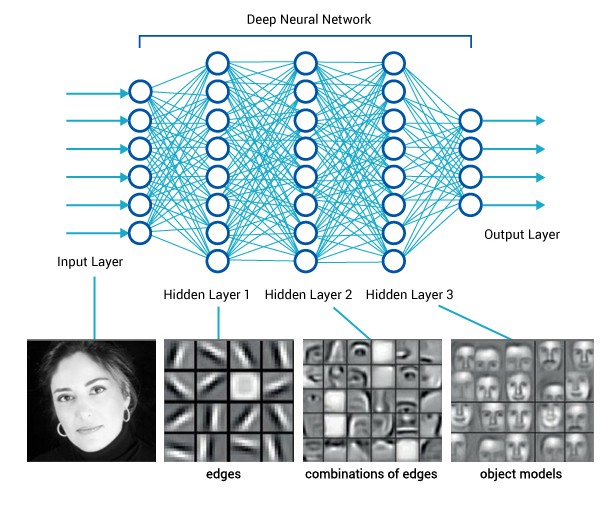
\includegraphics[scale=0.5]{Figures/2/deeplearning.jpeg}}
	\caption{ตัวอย่างการทำงานของการเรียนรู้เชิงลึก}{ที่มา: https://catalystsecure.com/blog/2017/07/deep-learning-in-e-discovery-moving-past-the-hype/}
	\label{fig:deep learning}
\end{figure}
\newpage
\section{ความรู้พื้นฐานเกี่ยวกับการเรียนรู้ของเครื่อง (Machine Learning)}
การเรียนรู้ของเครื่อง \cite{machinelearning} คือการทำให้คอมพิวเตอร์สามารถเรียนรู้ได้ด้วยตัวเองจากข้อมูลที่มีอยู่ ถ้าให้เปรียบเทียบแบบเห็นภาพชัดเจนคือเราเป็นครู คอมพิวเตอร์เป็นนักเรียนและความรู้เป็นข้อมูล แต่เดิมเราอยากสอนอะไรนักเรียน เราก็กางหนังสือแล้วถ่ายทอดความรู้ให้กับเด็ก ๆ ซึ่งนักเรียนก็จะเข้าใจความรู้นั้นเป็นก้อน แต่การเรียนรู้ของเครื่องคือการทำให้นักเรียนสามารถใช้ความรู้ (ข้อมูลที่ตัวเองมี) ในการวิเคราะห์ เชื่อมโยง คาดการณ์และประมวลผลได้ด้วยตัวเอง โดยไม่ต้องรอให้เราสอน

การเรียนรู้ของเครื่องมีรูปแบบการเรียนรู้ 3 รูปแบบ ดังนี้
\begin{itemize}[label={--}]
	\item การเรียนรู้แบบได้รับคำแนะนำ (Supervised learning)
	      เวลาป้อนข้อมูลให้กับคอมพิวเตอร์ (Input) เช่น รูปเสือ แต่คอมพิวเตอร์มันยังไม่รู้ว่าเป็นรูปเสือ เราก็ต้องบอกมันก่อน แล้วคอมพิวเตอร์ก็จะไปวิเคราะห์ (Feature Extraction) ว่า เสือเป็นสัตว์ 4 ขา มี 2 หู 1 หาง เป็นต้น จากนั้นคอมพิวเตอร์ก็นำข้อมูลดังกล่าวไปประมวลผล/จัดหมวดหมู่ (Classification) เพื่อให้หลังจากนี้มันสามารถแยกออกได้ว่าอะไรคือเสือ อะไรไม่ใช่เสือ
	
				\begin{figure}[H]
					\fbox{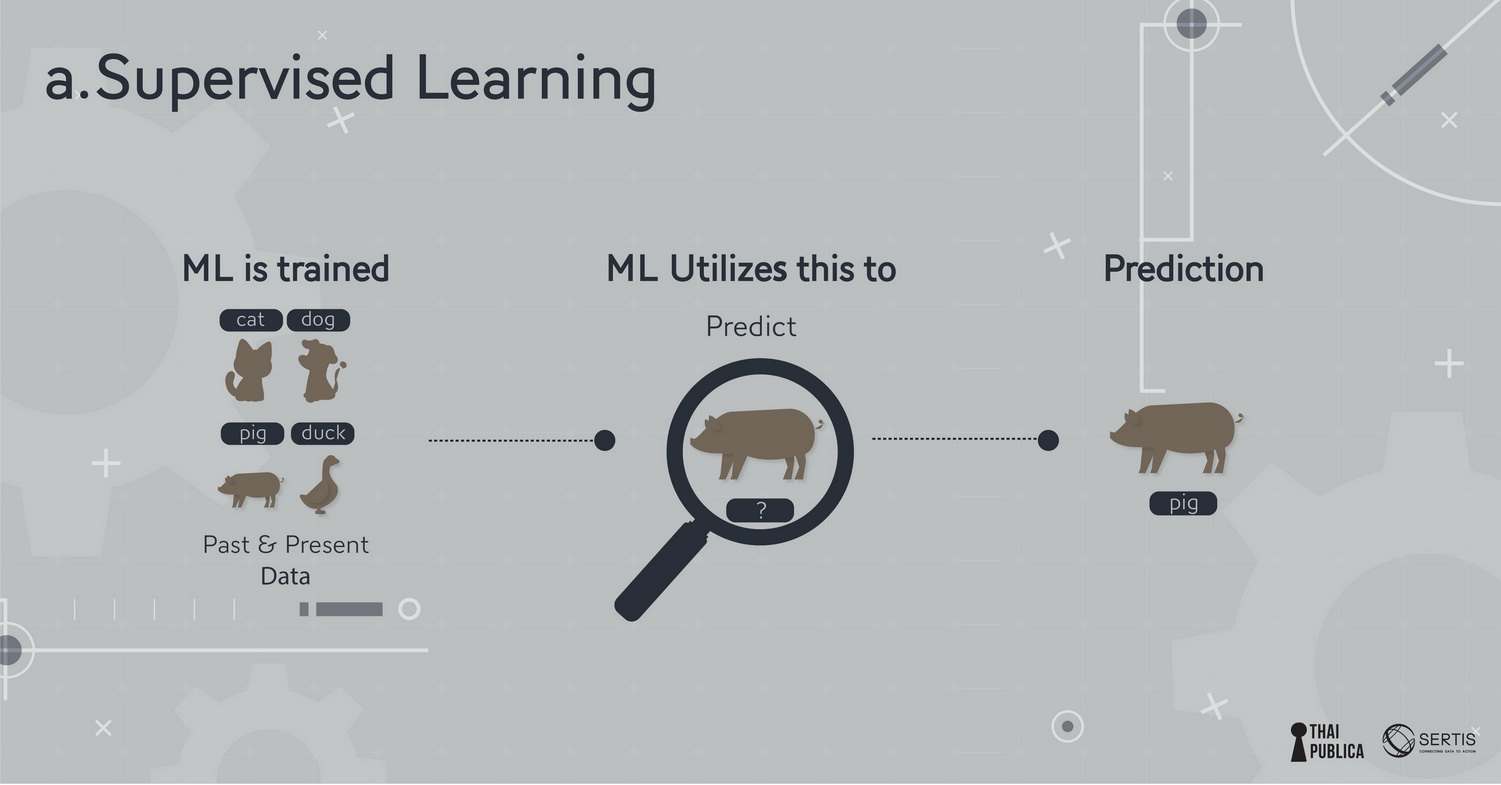
\includegraphics[width=\columnwidth]{Figures/2/7.jpg}}
					\caption{โมเดลที่ถูกสอนแบบ supervised learning}{ที่มา: https://thaipublica.org/2017/07/data-driven-society12/}
					\label{Fig:neural}
				\end{figure}
	
\item การเรียนรู้แบบไม่ได้รับคำแนะนำ (Unsupervised learning)
	      รูปแบบนี้เรียกได้ว่าตรงกันข้ามกับรูปแบบแรก มันคือการที่เราป้อนข้อมูล (Input) รูปเสือเข้าไป แต่ไม่ได้บอกมันว่ารูปที่ป้อนเข้าไปเป็นรูปเสือ เมื่อคอมพิวเตอร์มันเอาไปวิเคราะห์ (Feature Extraction) มันก็วิเคราะห์ได้นะว่ารูปที่ใส่เข้าไปมีลักษณะยังไง แต่คราวนี้มันไม่สามารถเอาไปประมวล/จัดหมวดหมู่ (Classification) ได้แล้ว มันจะใช้วิธีการแบ่งกลุ่มแทน (Clustering) ซึ่งคอมพิวเตอร์มันก็จะเอารูปเสือไปอยู่กับแมว สุนัข หรือสัตว์อื่น ๆ ที่มี 4 ขา มี 2 หู 1 หาง เหมือนกัน
				\begin{figure}[H]
					\fbox{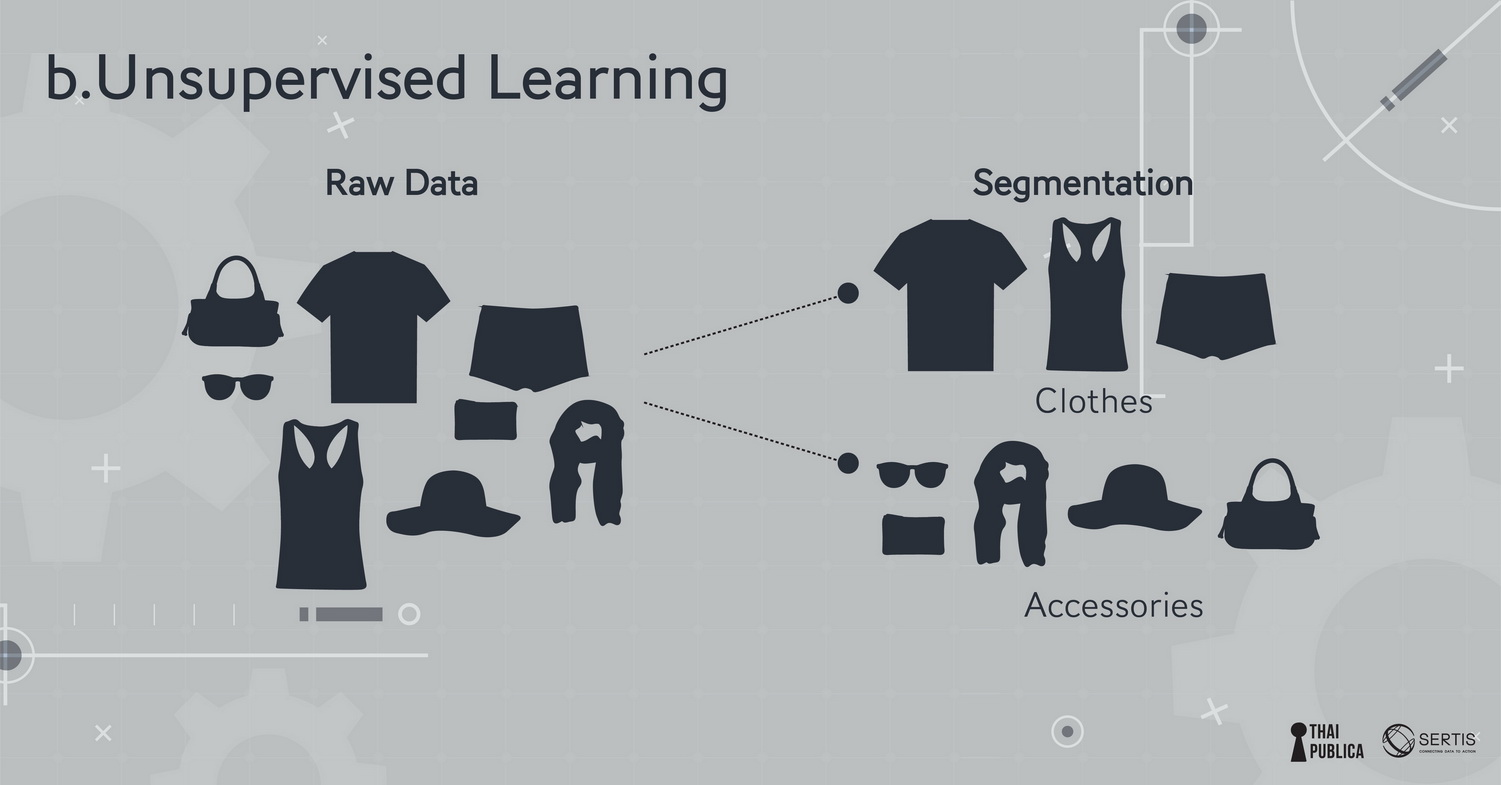
\includegraphics[width=\columnwidth]{Figures/2/8.jpg}}
					\caption{โมเดลที่ถูกสอนแบบ unsupervised learning}{ที่มา: https://thaipublica.org/2017/07/data-driven-society12/}
					\label{Fig:neural}
				\end{figure}
		\item การเรียนรู้แปบเสริมกำลัง (Reinforcement learning)
	      สามารถอธิบายได้ว่า เป็นการที่เรากำหนดเงื่อนไขบางอย่างให้กับคอมพิวเตอร์ แล้วทำให้คอมพิวเตอร์เอาชนะหรือทำตามเงื่อนไขนั้นให้ได้ ยกตัวอย่างเช่น Alpha Go เงื่อนไขของการเล่นหมากล้อมคือ ใช้หมากของตนล้อมพื้นที่บนกระดาน เพื่อให้ได้ดินแดนมากกว่าคู่ต่อสู้ ทีนี้ Alpha Go ก็จะเรียนรู้ด้วยตัวมันเองผ่านการจำลองการแข่งขันเป็นแสน ๆ ล้าน ๆ รอบ เพื่อให้รู้ว่า ถ้าหากคู่ต่อสู้เดินหมากนี้ ตัวมันเองจะเดินหมากไหนเพื่อให้บรรลุเงื่อนไขที่กำหนดไว้ให้ นั่นคือการยึดพื้นที่บนกระดานให้ได้มากที่สุด
				\begin{figure}[H]
					\fbox{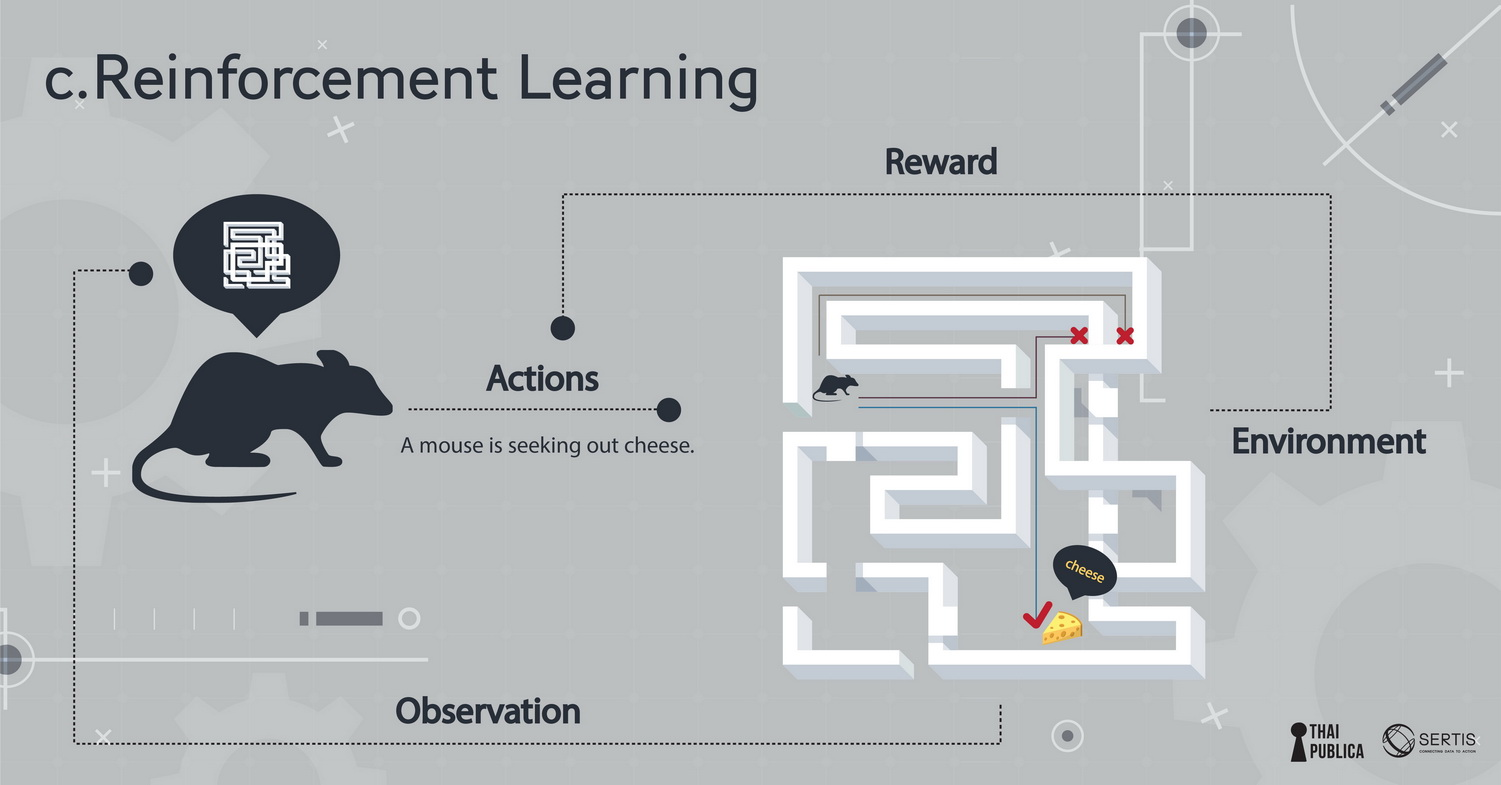
\includegraphics[width=\columnwidth]{Figures/2/un.jpg}}
					\caption{โมเดลที่ถูกสอนแบบ Reinforcement learning}{ที่มา: https://thaipublica.org/2017/07/data-driven-society12/}
					\label{Fig:neural}
				\end{figure}
			\end{itemize}

\section{ความรู้พื้นฐานเกี่ยวกับโครงข่ายประสาทเทียม (Neural Network)}
โครงข่ายประสาทเทียมคือโครงข่ายประสามเทียมที่เป็นการจำลองมาจากสมองของมนุษย์ โดยสมองของเรานั้นจะมีหน่วยประมวลผลขนาดเล็กอยู่เป็นจำนวนมาก และเชื่อมโยงกันด้วยโครงข่ายประสาท ช่วยให้มนุษย์สามารถเรียนรู้และคิดวิเคราะห์ได้อย่างรวดเร็ว แต่ในส่วนคอมพิวเตอร์นั้นไม่ได้มีโครงข่ายที่ซับซ้อนเหมือนกับสมองของมนุษย์ มันมีหน้าที่เพียงรันโปรแกรมตามคำสั่งของมนุษย์เท่านั้น ดังนั้นเมื่อต้องการให้มันทำการเรียนรู้บางอย่าง จึงเป็นเรื่องยากในรูปแบบปกติ จึงเกิดการจำลองแนวทางการเรียนรู้ของมนุษย์ไปสู่คอมพิวเตอร์ด้วยโครงข่ายประสาทเทียม \cite{neural}

โดยส่วนที่เล็กที่สุดของโครงข่ายประสาทเทียมคือ Neuron ทำหน้าที่คำนวนข้อมูลรับเข้าเพื่อให้ได้ผลลัพธ์ออกไป โดยในรูปที่ \ref{Fig:neural} มีส่วนประกอบสำคัญดังนี้
\begin{itemize}[label={--}]
	\item Input หรือค่าที่ส่งเข้ามาที่ Neuron โดยจะมีขาที่เข้ามาได้หลายขา ขึ้นอยู่กับเราจะสร้าง
	\item Weight เป็นการให้น้ำหนักของขาแต่ละที่ส่งเข้ามา โดยมีค่าระหว่าง 0-1 เมื่อเริ่มต้นจะเป็นการ Random ขึ้นมา จากนั้นตัว Neuron เมื่อทำการเรียนรู้จะเป็นการปรับ weight ตัวเอง เพื่อให้มันได้คำตอบที่ใกล้เคียงที่สุด
	\item Bias คือค่าที่จะช่วยเข้ามาทำให้ค่าที่เข้ามาอยู่ในระหว่าง 0 - 1 ได้ โดยจะเป็นเลข random และปรับทุกครั้งที่เรียนรู้
	\item Output คือผลลัพธ์
	\item Back Propagation คือการที่ Neuron นำค่า Error ของ Output ที่ได้ กับ Output ที่เราสั่งให้มันเรียนรู้ นำไปปรับ Weight และ Bias ให้เกิดผลลัพธ์ที่ถูกต้องตามที่ได้เรียนรู้มา
\end{itemize}
\begin{figure}[H]
	\fbox{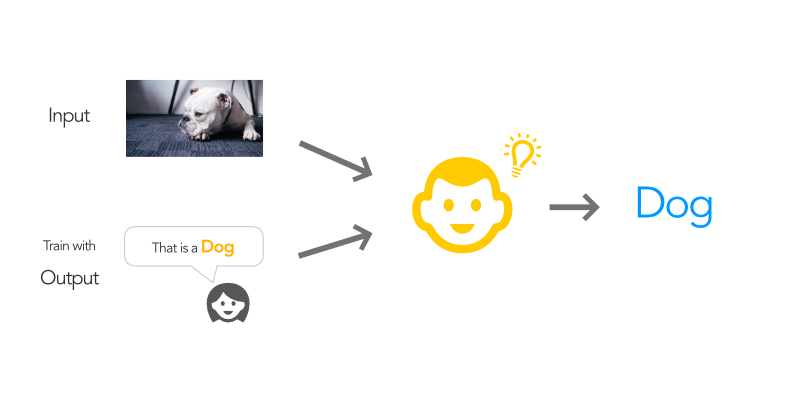
\includegraphics[width=\columnwidth]{Figures/2/neural.png}}
	\caption{ตัวอย่างของโครงข่ายประสาท}{ที่มา: https://coladev.com/machine-learning/neural-network/2017/02/22/neural-network-basic}
	\label{Fig:neural}
\end{figure}




	\section{ความรู้พื้นฐาน Firebase }
				Firebase  \cite{fi} คือ Platform ที่รวบรวมเครื่องมือต่าง ๆ สำหรับการจัดการในส่วนของ Backend หรือ Server side ซึ่งทำให้สามารถ Build Mobile Application ได้อย่างมีประสิทธิภาพ และยังลดเวลาและค่าใช้จ่ายของการทำ Server side หรือการวิเคราะห์ข้อมูล โดยมีทั้งเครื่องมือที่ฟรี และเครื่องมีที่มีค่าใช้จ่าย \cite{fi}
เครื่องมือ Firebase มีดังนี้
				\begin{enumerate}
					\item  Cloud Firestore คือ เครื่องมือ Database ที่เป็นลักษณะเป็น NoSQL โดยนำข้อดีของ Realtime Database ของ Firebase มาพัฒนาต่อ
					\item  Authentication  คือ  เครื่องมือ  Authentication ซึ่งคลอบคลุมทั้ง email-password, phone ไปจนถึง facebook, twitter, github สำหรับการ Login 
					\item  Hosting คือ hosting สำหรับ single-page web app, landing page website ซึ่งจัดการการ Deploy  และมีการติดตั้ง SSL ให้กับในส่วน Custom Domain  
					\item  Crashlytics ช่วยจัดการ Issue ต่าง ๆ และสามารถตรวจจับ Crash ได้ว่าเกิดขึ้นที่การทำงานไหนใน Mobile App 
					\item  Performance Monitoring  โดยผู้พัฒนาสามารถดู Performance ของ Code และ Network
				\end{enumerate}

						
			
\chapter{การวิเคราะห์และออกแบบระบบ}

การวิเคราะห์และออกแบบระบบก่อนดำเนินการจริงเป็นอีกหนึ่งขั้นตอนที่มีความสำคัญมาก เพราะการวิเคราะห์และออกแบบระบบนั้นเป็นการกระทำที่ทำให้ผู้พัฒนาเห็นรายละเอียดส่วนย่อยของงานทั้งหมด เพิ่มประสิทธิภาพในการวางแผน การทำงาน และยังช่วยลดปัญหาที่อาจจะเกิดขึ้นในระหว่างพัฒนา เพื่อให้ระบบมีความสมบูรณ์มากยิ่งขึ้น เนื่องจากการวิเคราะห์และออกแบบระบบนั้นจะช่วยให้ให้บริการ จัดการทรัพยากรได้อย่างคุ้มค่าและตรงตามความต้องการของระบบ

การวิเคราะห์และออกแบบแอปพลิเคชันสแกนอาหาร ในบทนี้จะแบ่งออกเป็น 6 ข้นตอนเพื่อให้เห็นการดำเนินงานอย่างมีระบบ ในหัวข้อแรกจะนำเสนอภาพรวมของระบบ ก่อนจะนำเสนอเอกสารแสดงความต้องการของระบบซึ่งจะทำให้เห็นที่มาของเพจต่าง ๆ ในขั้นตอนของการออกแบบในหัวข้อที่สาม ส่วนหัวข้อที่เหลือจะแสดงแผนภาพการการทำงานของระบบโดยใช้ UML diagram ซึ่งประกอบไปด้วย Use Case, Class และ Sequence Diagram เพื่อแสดงรายละเอียดของระบบก่อนนำไปเขียนคำสั่งด้วยภาษาโปรแกรมในบทต่อไป

\begin{enumerate}[label=3.\arabic*]
	\item โครงสร้างภาพรวมของระบบ (System Architecture) เป็นการออกแบบภาพรวมและเทคโนโลยีของระบบ
	\item System Requirements คือ ความต้องการหรือสิ่งที่ระบบควรจะทำ หรือหน้าที่หลักของ
	ระบบที่จะต้องทำ
	\item User Interface Design เป็นการออกแบบส่วนต่อประสานกับผู้ใช้
	\item Use Case Diagram เป็นแผนภาพที่ใช้แสดงให้ทราบว่าระบบทำงานหรือมีหน้าที่ใดบ้าง
	\item Class Diagram เป็นแผนภาพที่ใช้แสดง Class และความสัมพันธ์ระหว่าง Class
	\item Sequence Diagram เป็นแผนภาพที่ใช้แสดงให้เห็นถึงการตอบโต้ข้อมูลระหว่างคลาส เรียงตามลำดับของเวลาที่เกิดเหตุการณ์จากน้อยไปมาก
\end{enumerate}	

\section{โครงสร้างการทำงานข้อระบบ}
 ระบบแอปพลิเคชัน What is that มีโครงสร้างการทำงานดังรูปที่ 3.1
   	\begin{figure}[H]
   		\centering
   		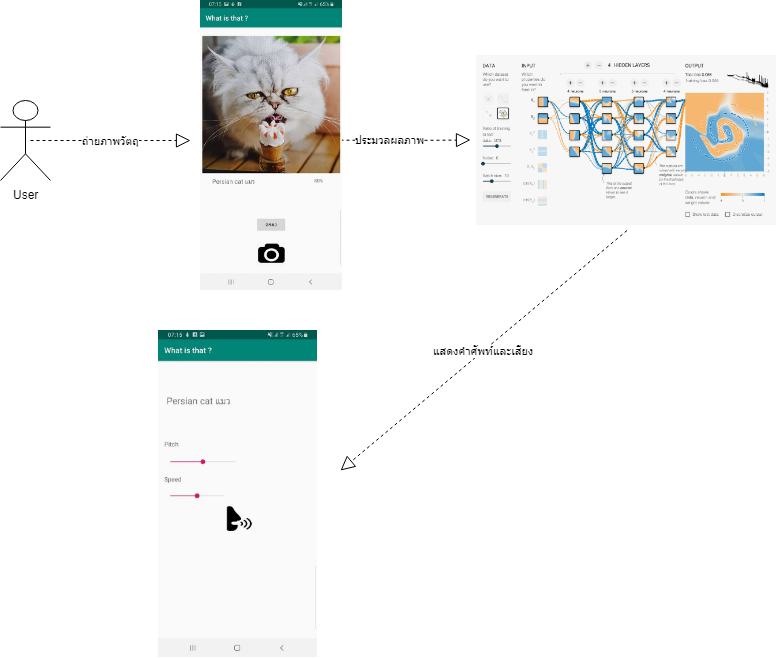
\includegraphics[width=\textwidth]{Figures/3/architecture/31.png}
   		\caption{โครงสร้างการทำงานข้อระบบ}
   		\label{Fig:architecture}
   	\end{figure}
   
	 		จากรูปที่ \ref{Fig:architecture} สามารถอธิบายโครงสร้างการทำงานของระบบได้ดังนี้ ผู้ใช้งานต้องทำการถ่ายต้องการ ระบบจะนำภาพไปเปรียบเทียบกับข้อมูลที่ผ่านกระบวนการประมวลผลภาพ
 จากนั้นระบบจะแสดงคำศัพท์ภาษาอังกฤษของภาพนั้นๆแล้วแปลงข้อความที่ได้เป็นเสียงพูด 
   

\section{System Requirements}
		\subsection{Functional Requirements} 
แอปพลิเคชัน What is that แบ่งตามประเภทผู้ใช้งานดังนี้ 
\begin{enumerate}
		\item ผู้ใช้งาน
			\begin{itemize}[label={--}]
				\item สามารถระบุภาพภ่ายได้
				\item สามารถดูคำศัพท์และคำแปลได้
				\item สามารถฟังเสียงของคำศัพท์นั้นได้่
				\item สามารถเลือกระดับความเร็วในการออกเสียงได้ 
				\item สามารถลือกโทนเสียงได้
			\end{itemize}
			\end{enumerate}

		\subsection{Non-functional Requirements}
		\begin{enumerate}
		\item แอนดรอยด์แอปพลิเคชัน
		\begin{itemize}[label={--}]
			\item  แอปพลิเคชันสามารถวิเคราะห์ภาพได้ภายในระยะเวลา 1 วินาที 
			\item  แอปพลิเคชันมีเสียงรองมากกว่า 1 ภาษา
		
		\end{itemize}
	\end{enumerate}
	
\section{User Interface Design}
ในการออกแบบ User Interface Design ของแอปพลิเคชันสแกนอาหาร ออกแบบมาให้มีลักษณะที่ใช้งานง่ายเพียงแค่ไม่กี่ขั้นตอน โดยสามารถโต้ตอบกับผู้ใช้ได้ 
\begin{itemize}[label={--}]

\item การออกแรกของแอพพลิเคชัน

				\begin{figure}[H]
					\centering
					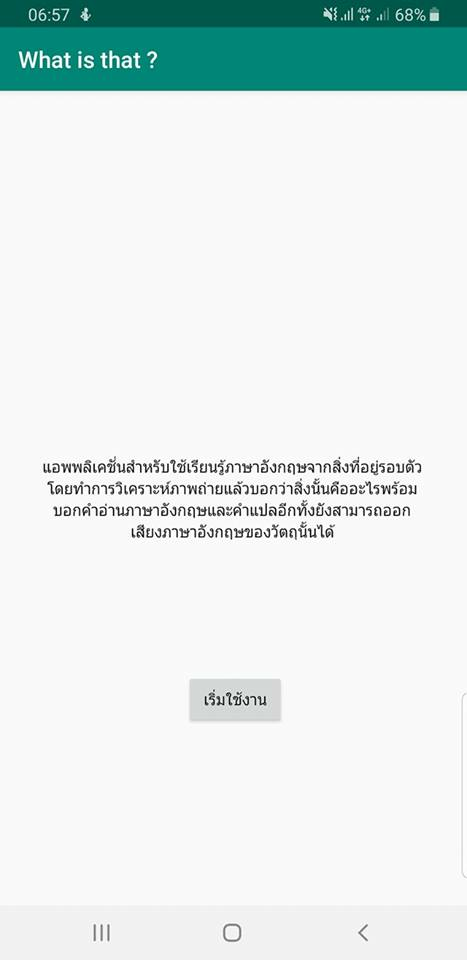
\includegraphics[width=0.2\textwidth]{Figures/3/UIDESIGN/main.png}
					\caption{หน้าแรก}
					\label{Fig:1}
				\end{figure}
				จากภาพที่ \ref{Fig:1}แสดงหน้าหลักและอธิบายรายละเอียดของตัวแอพพลิเคชั่น
			\end{enumerate}
		\end{itemize}

				\newpage

				\begin{itemize}[label={--}]

\item การออกแบบหน้าจอวิเคราะห์ภาพ 
	\begin{figure}[H]
					\centering
					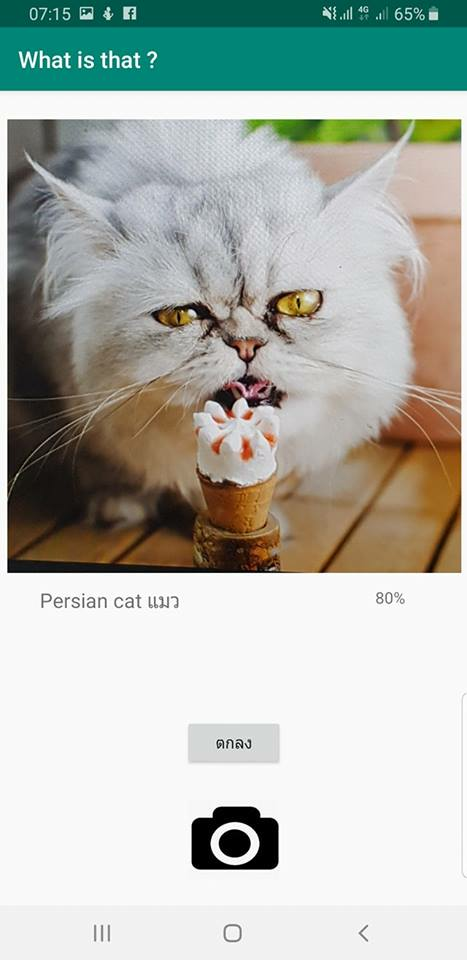
\includegraphics[width=0.2\textwidth]{Figures/3/UIDESIGN/pic.png}
					\caption{หน้าระบุถาพถ่ายที่เลือก}
					\label{Fig:2}
				\end{figure}
				จากภาพที่ \ref{Fig:2} เมื่อผู้ใช้ทำการกดที่ปุ่ม ตกลง ระบบจะทำการวิเคราห์ภาพแล้วแสดงคำศัพท์ภาษาอังกฤษของภาพนั้นๆ หรือกดที่รูปกล้องเพื่อกลับไปถ่ายภาพวัตถุใหม่อีกครั้ง
			\end{itemize}
	\begin{itemize}[label={--}]
\item การออกแบบหน้าจอเสียงพูด 
				\begin{figure}[H]
								\centering
								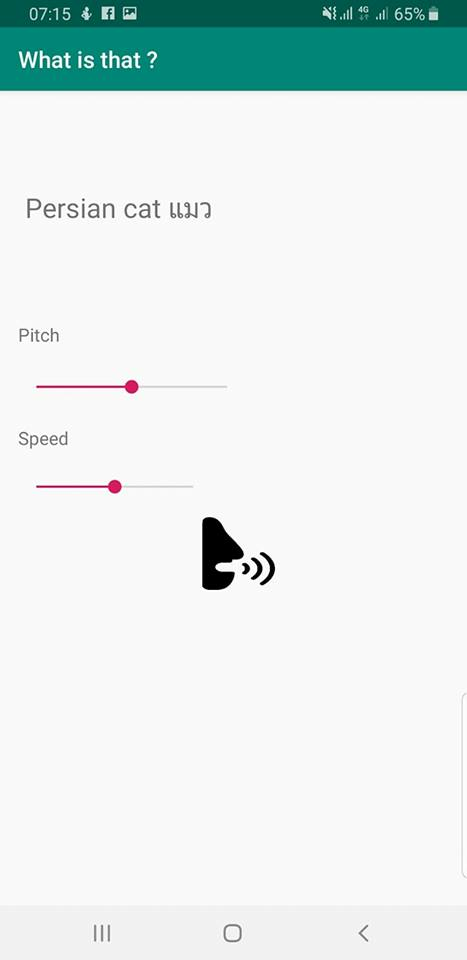
\includegraphics[width=0.2\textwidth]{Figures/3/UIDESIGN/speak.png}
								\caption{หน้าจอ แดชบอร์ด}
								\label{Fig:5}
							\end{figure}
							จากภาพที่ \ref{Fig:5} ในหน้านี้จะนำคำศัพท์ที่ได้มาประมวลผล และสามาถกดเพื่ออ่านออกเสียงคำศัพท์นั้นเป็นภาษาอังกษได้ อีกทั้งยังสมารถเลือกความเร็วในการอ่านออกเสียงได้เพื่อให้ผู้ใช้สามารถฟังได้ง่ายขึ้น
						\end{itemize}
							\newpage

\begin{itemize}[label={--}]

								
									\end{itemize}


										\newpage

\section{Use Case Diagram}
	Use Case Diagram เป็นแผนผังเพื่อแสดงฟังก์ชันแสดงการทำงานของระบบโดยรวม แสดงส่วนประกอบในระบบและกิจกรรมที่เกิดขึ้นในระบบซึ่งในระบบระบบกองทุนเงินให้กู้ยืมเพื่อการศึกษา คณะวิทยาศาสตร์ มหาวิทยาลัยอุบลราชธานี ผู้ใช้จำเป็นต้องเข้าสู่ระบบเพื่อใช้งานระบบ สัญลักษณ์ที่ใช้ในการเขียน Use Case Diagram แสดงในตารางที่ \ref{tab:use-case2}
	\begin{table}[H]
		\caption{สัญลักษณ์ของ Use case Diagram}
		\label{tab:use-case2}
		\begin{tabular}{|c|p{10cm}|}
		\hline
		\textbf{สัญลักษณ์} & \multicolumn{1}{c|}{\textbf{การใช้งาน}} \\ \hline
		\raisebox{-\totalheight}{Use case}
		& \setstretch{1.5} {Use case คือส่วนย่อยของระบบงาน แทนด้วยวงรีและชื่อของ Use case ภายในวงรี} \\ \hline
		\raisebox{-\totalheight}{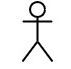
\includegraphics[height=1.5cm]{Figures/table/use-case/2}}
		& \setstretch{1.5} {Actor คือบุคคลหรือระบบงานอื่นที่ใช้งานระบบหรือได้รับประโยชน์จากระบบซึ่งอยู่ภายนอกระบบ แทนด้วยรูปคนและมีชื่อบทบาทการใช้งานระบบ} \\ \hline
		\raisebox{-\totalheight}{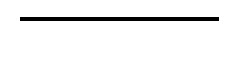
\includegraphics[width=3cm]{Figures/table/use-case/3}}
		& \setstretch{1.5} {เส้นตรงที่แสดงถึงการใช้งาน Use case ของผู้กระทำ} \\ \hline
		\raisebox{-\totalheight}{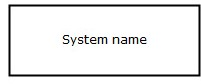
\includegraphics[width=0.3\textwidth]{Figures/table/use-case/4}}
		& \setstretch{1.5} {กรอบสี่เหลี่ยมแสดงถึงขอบเขตของระบบโดยแสดงชื่อระบบภายในหรือด้านบนกรอกสี่เหลี่ยม Use case อยู่ภายในกรอบสี่เหลี่ยม และ actor อยู่ภายนอกกรอบสี่เหลี่ยม} \\ \hline
		\raisebox{-\totalheight}{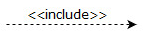
\includegraphics[width=0.3\textwidth]{Figures/table/use-case/5}}
		& \setstretch{1.5} {ความสัมพันธ์แบบ <<includes>> แสดงว่า Use case หนึ่งดำเนินการตามขั้นตอนของ Use case อื่น โดยแทนด้วยสัณลักษณ์ลูกศรเส้นประ ซึ่ง Use case ที่หางลูกศรเรียกใช้งาน Use case ที่หัวลูกศรทุกครั้งที่มีการทำงาน} \\ \hline
		\raisebox{-\totalheight}{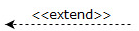
\includegraphics[width=0.3\textwidth]{Figures/table/use-case/6}}
		& \setstretch{1.5} {ความสัมพันธ์แบบ <<extend>> แสดงว่า Use case หนึ่งดำเนินการตามขั้นตอนของ Use case อื่น โดยแทนด้วยสัญลักษณ์ลูกศรเส้นประ ซึ่ง Use case ที่หัวลูกศรเรียกใช้งาน Use case ที่หางลูกศร แต่การใช้งานไม่จำเป็นต้องเกิดขึ้นทุกครั้งขึ้นอยู่กับเงื่อนไขระหว่างการทำงาน} \\ \hline
		\end{tabular}
	\end{table}

	\begin{figure}[H]
		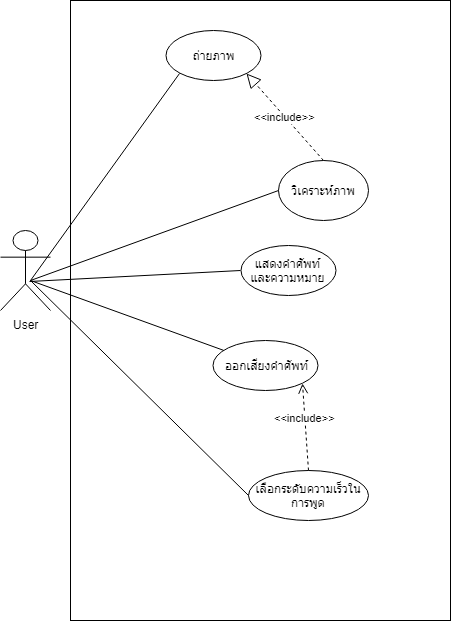
\includegraphics[width=0.9\textwidth]{Figures/3/usecase/usecase.png}
		\caption{Use Case Diagram ของแอปพลิเคชัน What is that}
		\label{Fig:usecase}
	\end{figure}
	
	\begin{table}[H]
		\centering
		\caption{อธิบาย Use Case หน้าที่ของระบบโดยทุกการทำงานจะต้องอาศัยการเข้าสู่ระบบทุกครั้ง ในภาพที่ \ref{Fig:usecase}}
		\label{tab:usecase}
		\resizebox{\totalheight}{!}{\textwidth}{%
			\begin{tabular}{|c|p{8cm}|}
				\hline
				\multicolumn{1}{|c|}{\textbf{Use Case}} & \multicolumn{1}{c|}{\textbf{คำอธิบาย}} \\ \hline
				สแกนอาหาร & สมาชิกสามารถสแกนอาหารแต่ไม่จำเป็นต้องบันทึกข้อมูลการบริโภคทุกครั้ง \\ \hline
				บันทึกแคลลอรี่ น้ำตาล โซเดียมและไขมัน &  การบันทึกข้อมูลการบริโภคสมาชิกไม่จำต้องทำการสแกนทุกครั้ง \\ \hline
				เข้าสู่ระบบ & สมาชิกสามารถทำการเข้าสู่ระบบได้ \\ \hline
				ออกจากระบบ & สมาชิกจะต้องทำการเข้าสู่ระบบก่อนจึงจะสามารถออกจากระบบได้ \\ \hline
				ดูข้อมูลการบริโภครูปแบบวัน สัปดาห์และเดือน & หลังจากสมาชิกทำการเข้าสู่ระบบแล้วสมาชิกสามารถดูข้อมูลการบริโภคในรูปแบบวัน
				 สัปดาห์และเดือนได้  \\ \hline
				ลบอาหารที่เพิ่ม &  สมาชิกสามารถลบอาหารที่เพิ่มเข้ามาได้ด้วยการเลือกที่รายการอาหาร \\ \hline
				เพิ่มอาหารที่ไม่มีในระบบ &  สมาชิกสามารถเพิ่มอาหารที่ไม่มีในระบบเองได้   \\ \hline
			\end{tabular}%
		}
	\end{table}
	% Please add the following required packages to your document preamble:
	% \usepackage{graphicx}
	\begin{table}[H]
		\centering
		\caption{Use Case สแกนอาหาร}
		\label{tab:usecase}
		\resizebox{\totalheight}{!}{\textwidth}{%
			\begin{tabular}{|p{10cm}|p{10cm}|}
				\hline
				\multicolumn{1}{|c|}{\textbf{Use Case Title : สแกนอาหาร}} & \multicolumn{1}{c|}{\textbf{Use case Id : 1 }} \\ \hline
				\multicolumn{2}{|p{\linewidth}|}{Primary Actor : สมาชิก} \\ \hline
			    \multicolumn{2}{|p{\linewidth}|}{Main Flow : สมาชิกจะต้องทำการเข้าสู่ระบบก่อนจึงจะสามารถทำการสแกนได้} \\ \hline
			    \multicolumn{2}{|p{\linewidth}|}{Exceptional Flow ที่ 1 : หากผู้ใช้ไม่เชื่อมต่ออินเทอร์เน็ต จะไม่สามารถทำการสแกนได้} \\ \hline
			\end{tabular}%
		}
	\end{table}
	\begin{table}[H]
		\centering
		\caption{Use Case บันทึกแคลลอรี่ น้ําตาล โซเดียมและไขมัน}
		\label{tab:usecase}
		\resizebox{\totalheight}{!}{\columnwidth}{%
			\begin{tabular}{|p{7cm}|p{7cm}|}
				\hline
				\multicolumn{1}{|c|}{\textbf{Use Case Title : บันทึกแคลลอรี่ น้ําตาล โซเดียมและไขมัน}} & \textbf{Use case Id : 2 } \\ \hline
				\multicolumn{2}{|l|}{Primary Actor : สมาชิก} \\ \hline
				\multicolumn{2}{|p{\linewidth}|}{Main Flow : หากสมาชิกต้องการบันทึกสมาชิกสามารทำการสแกนหรือบันทึกจากอาหารที่เพิ่มเองได้  } \\ \hline
				\multicolumn{2}{|p{\linewidth}|}{Exceptional Flow ที่ 1 : หากสมาชิกไม่เชื่อมต่ออินเทอร์เน็ต จะไม่สามารถทำการบันทึกข้อมูลอาหารได้} \\ \hline
			\end{tabular}%
		}
	\end{table}

	\begin{table}[H]
		\centering
		\caption{Use Case เข้าสู่ระบบ}
		\label{tab:usecase}
		\resizebox{\totalheight}{!}{\textwidth}{%
			\begin{tabular}{|p{7cm}|p{7cm}|}
				\hline
				\multicolumn{1}{|c|}{\textbf{Use Case Title : ดาวน์โหลดเอกสาร}} & \textbf{Use case Id : 3 } \\ \hline
				\multicolumn{2}{|l|}{Primary Actor : สมาชิก} \\ \hline
				\multicolumn{2}{|p{\linewidth}|}{Main Flow : สมาชิกต้องทำการสมัครสมาชิกก่อนจึงจะสามารถทำการเข้าสู่ระบบได้				} \\ \hline
				\multicolumn{2}{|p{\linewidth}|}{Exceptional Flow ที่ 1 : หากสมาชิกไม่เชื่อมต่ออินเทอร์เน็ต จะไม่สามารถทำการเข้าสู่ระบบได้} \\ \hline
				\multicolumn{2}{|p{\linewidth}|}{Exceptional Flow ที่ 2 : หากสมาชิกไม่ทำการสมัครสมาชิกจะไม่สามารถทำการเข้าสู่ระบบได้ } \\ \hline
			\end{tabular}%
		}
		\end{table}
		
		\begin{table}[H]
			\centering
			\caption{Use Case ออกจากระบบ}
			\label{tab:usecase}
			\resizebox{\totalheight}{!}{\textwidth}{%
				\begin{tabular}{|p{10cm}|p{10cm}|}
					\hline
					\multicolumn{1}{|c|}{\textbf{Use Case Title : ออกจากระบบ}} & \multicolumn{1}{c|}{\textbf{Use case Id : 4 }} \\ \hline
					\multicolumn{2}{|l|}{Primary Actor : สมาชิก} \\ \hline
					\multicolumn{2}{|p{\linewidth}|}{Main Flow : สมาชิกจะต้องทำการเข้าสู่ระบบก่อนจึงจะสามารถออกจากระบบได้ } \\ \hline
					\multicolumn{2}{|p{\linewidth}|}{Exceptional Flow ที่ 1 : หากผู้ใช้ไม่ทำการเข้าสู่ระบบ จะไม่สามารถออกจากระบบได้ } \\ \hline
				\end{tabular}%
			}
		\end{table}
		
		\begin{table}[H]
			\centering
			\caption{Use Case ดูข้อมูลการบริโภครูปแบบวัน สัปดาห์และเดือน}
			\label{tab:usecase}
			\resizebox{\totalheight}{!}{\textwidth}{%
				\begin{tabular}{|c|p{10cm}|}
					\hline
					\multicolumn{1}{|c|}{\textbf{Use Case Title : ดูข้อมูลการบริโภครูปแบบวัน สัปดาห์และเดือน}} & \multicolumn{1}{c|}{\textbf{Use case Id : 5 }} \\ \hline
					\multicolumn{2}{|l|}{Primary Actor : สมาชิก} \\ \hline
					\multicolumn{2}{|p{\linewidth}|}{Main Flow : เมื่อสมาชิกทำการเข้าสู่ระบบแล้ว สมาชิกสามารถดูข้อมูลการบริโภคในรูปแบบวัน สัปดาห์และเดือนได้ } \\ \hline
					\multicolumn{2}{|p{\linewidth}|}{Exceptional Flow ที่ 1 : หากผู้ใช้ไม่เชื่อมต่ออินเทอร์เน็ต จะไม่สามารถดูข้อมูลการบริโภคในรูปแบบวัน สัปดาห์และเดือนได้} \\ \hline
				\end{tabular}%
			}
		\end{table}
	
		\begin{table}[H]
			\centering
			\caption{Use Case ลบอาหารที่เพิ่ม}
			\label{tab:usecase}
			\resizebox{\totalheight}{!}{\textwidth}{%
				\begin{tabular}{|c|p{10cm}|}
					\hline
					\multicolumn{1}{|c|}{\textbf{Use Case Title : ลบอาหารที่เพิ่ม}} & \multicolumn{1}{c|}{\textbf{Use case Id : 6 }} \\ \hline
					\multicolumn{2}{|l|}{Primary Actor : สมาชิก} \\ \hline
					\multicolumn{2}{|p{\linewidth}|}{Main Flow :  สมาชิกสามารถทำการลบอาหารได้ด้วยการเลือกที่เมนูอาหาร} \\ \hline
					\multicolumn{2}{|p{\linewidth}|}{Exceptional Flow ที่ 1 : หากสมาชิกไม่เชื่อมต่ออินเทอร์เน็ต จะไม่สามารถทำการลบอาหารได้} \\ \hline
				\end{tabular}%
			}
		\end{table}	
		
		\begin{table}[H]
			\centering
			\caption{Use Case เพิ่มอาหารท่ีไม่มีในระบบ}
			\label{tab:usecase}
			\resizebox{\totalheight}{!}{\textwidth}{%
				\begin{tabular}{|c|p{10cm}|}
					\hline
					\multicolumn{1}{|c|}{\textbf{Use Case Title : เพิ่มอาหารท่ีไม่มีในระบบ}} & \multicolumn{1}{c|}{\textbf{Use case Id : 7 }} \\ \hline
					\multicolumn{2}{|l|}{Primary Actor : สมาชิก} \\ \hline
					\multicolumn{2}{|p{\linewidth}|}{Main Flow :  สมาชิกสามารถเพิ่มอาหารที่ไม่มีในระบบได้ด้วยการกดปุ่ม ADD  } \\ \hline
					\multicolumn{2}{|p{\linewidth}|}{Exceptional Flow ที่ 1 : หากสมาชิกไม่เชื่อมต่ออินเทอร์เน็ต จะไม่สามารถเพิ่มอาหารได้} \\ \hline
				\end{tabular}%
			}
		\end{table}	
%		\begin{table}[H]
%			\centering
%			\caption{Use Case สมัครสมาชิก}
%			\label{tab:usecase}
%			\resizebox{\totalheight}{!}{\textwidth}{%
%				\begin{tabular}{|c|p{10cm}|}
%					\hline
%					\multicolumn{1}{|c|}{\textbf{Use Case Title : สมัครสมาชิก}} & \multicolumn{1}{c|}{\textbf{Use case Id : 8 }} \\ \hline
%					\multicolumn{2}{|l|}{Primary Actor : นักศึกษา} \\ \hline
%					\multicolumn{2}{|l|}{Stakeholder Actor : -} \\ \hline
%					\multicolumn{2}{|p{\linewidth}|}{Main Flow : เมื่อนักศึกษาต้องการใช้งานระบบทั้งหมดของกองทุนจำเป็นต้องเข้าสู่ระบบก่อน หากยังไม่มีบัญชีสามารถสมัครได้โดยต้องกรอกข้อมูลอีเมลและรหัสผ่าน} \\ \hline
%					\multicolumn{2}{|p{\linewidth}|}{Exceptional Flow ที่ 1 : หากผู้ใช้ไม่เชื่อมต่ออินเทอร์เน็ต จะไม่สามารถสมัครสมาชิกได้} \\ \hline
%				\end{tabular}%
%			}
%		\end{table}	
%		 \begin{table}[H]
%		 	\centering
%		 	\caption{Use Case เข้าสู่ระบบ}
%		 	\label{tab:usecase}
%		 	\resizebox{\totalheight}{!}{\textwidth}{%
%		 		\begin{tabular}{|c|p{10cm}|}
%		 			\hline
%		 			\multicolumn{1}{|c|}{\textbf{Use Case Title : เข้าสู่ระบบ}} & \multicolumn{1}{c|}{\textbf{Use case Id : 9 }} \\ \hline
%		 			\multicolumn{2}{|l|}{Primary Actor : นักศึกษา} \\ \hline
%		 			\multicolumn{2}{|l|}{Stakeholder Actor : -} \\ \hline
%		 			\multicolumn{2}{|p{\linewidth}|}{Main Flow : เมื่อนักศึกษาต้องการใช้งานระบบทั้งหมดของกองทุนจำเป็นต้องเข้าสู่ระบบก่อนโดยต้องกรอกข้อมูลอีเมลและรหัสผ่าน} \\ \hline
%		 			\multicolumn{2}{|p{\linewidth}|}{Exceptional Flow ที่ 1 : หากผู้ใช้ไม่เชื่อมต่ออินเทอร์เน็ต จะไม่สามารถเข้าสู่ระบบได้} \\ \hline
%		 		\end{tabular}%
%		 	}
%		 \end{table}	
	
\newpage

\section{Class Diagram}
	Class Diagram คือแผนภาพที่ใช้แสดงคลาสและความสัมพันธ์ในแบบต่างๆ ระหว่างคลาส สัญลักษณ์ที่ใช้ในการเขียน Class Diagram แสดงในตารางที่ \ref{tab:class2} 
	\begin{center}
	\begin{table}[H]
		\centering
		\caption{สัญลักษณ์ของ Class Diagram}
		\label{tab:class2}
		\begin{tabular}{|c|p{10cm}|}
			\hline
			\textbf{สัญลักษณ์} & \multicolumn{1}{c|}{\textbf{การใช้งาน}} \\ \hline
			\raisebox{-\totalheight}{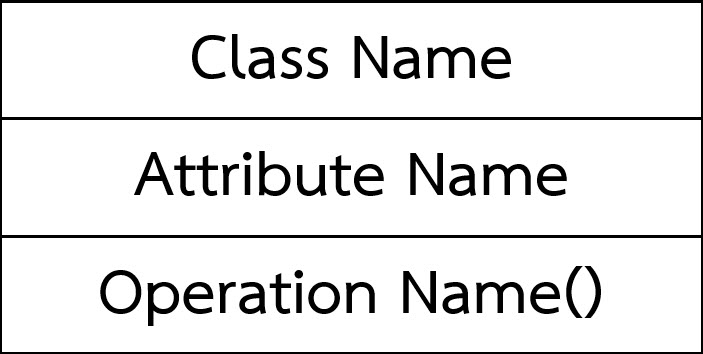
\includegraphics[width=0.3\textwidth]{Figures/table/class/11}}
			& \setstretch{1.5} {คลาส สัญลักษณ์แทนด้วยสี่เหลี่ยมแบ่งเป็น 3 ส่วน 
				ส่วนบน เป็นชื่อของ class ส่วนกลาง เป็นชื่อ Attribute และส่วนล่างเป็น Operation Name หรือ Method ใช้สำหรับเขียนฟังก์ชันในการทำงานของคลาสนั้น ๆ
				ชนิดของ Visibility ของ Method และ Attribute
				แบ่งเป็น 3 ชนิด ได้แก่
				\begin{enumerate}
					\item Public แทนสัญลักษณ์ด้วยเครื่องหมายบวก (+)
					\item Private แทนสัญลักษณ์ด้วยเครื่องหมายลบ (-)
					\item Protected แทนสัญลักษณ์ด้วยเครื่องหมายชาร์ป (#)
				\end{enumerate}
			} \\ \hline
			\raisebox{-\totalheight}{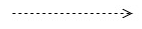
\includegraphics[width=0.3\textwidth]{Figures/table/class/1}}
			& \setstretch{1.5} {Dependency Relationship หมายความว่า คลาสที่อยู่ฝั่งต้นลูกศรสามารถเรียกใช้คลาสที่อยู่ฝั่งหัวลูกศร}
			\\ \hline
			\raisebox{-\totalheight}{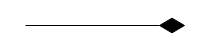
\includegraphics[width=0.35\textwidth]{Figures/3/Class/aggre}}
			& \setstretch{1.5} {Composition Relationship เป็นความสัมพันธ์ระหว่างออบเจ็กต์หรือคลาสแบบขึ้นต่อกันและมีความเกี่ยวข้องกันเสมอ} \\ \hline
			\raisebox{-\totalheight}{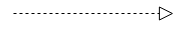
\includegraphics[width=0.3\textwidth]{Figures/3/Class/implement}}
			& \setstretch{1.5} {Realization Relationship เป็นความสัมพันธ์ระหว่าง Object หรือ Class ในลักษณะของการสืบทอดคุณสมบัติจาก Class หนึ่ง (Super class) ไปยังอีก Class หนึ่ง (Subclass)} \\ \hline
			\raisebox{-\totalheight}{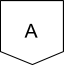
\includegraphics[width=50,height=50]{Figures/table/class/connector}}
			& \setstretch{1.5} {Connector เป็นสัญลักษณ์แทนด้วยรูปห้าเหลี่ยมและมีชื่ออยู่ตรงกลาง จะสร้างสัญลักษณ์นี้ไว้เมื่อต้องการเชื่อมต่อคลาสที่อยู่คนละหน้า} \\ \hline
		\end{tabular}
	\end{table}
	\end{center}

\newpage
	%IMAGE of class

	Class Diagram แสดงความสัมพันธ์ในรูปแบบต่างๆ ระหว่างคลาสของแอปพลิเคชันระบบกองทุนเงินให้กู้ยืมเพื่อการศึกษา คณะวิทยาศาสตร์ มหาวิทยาลัยอุบลราชธานี อธิบายได้ตามภาพที่ \ref{Fig:MainActivity20C} ดังต่อไปนี้
	

	\begin{figure}[H]

		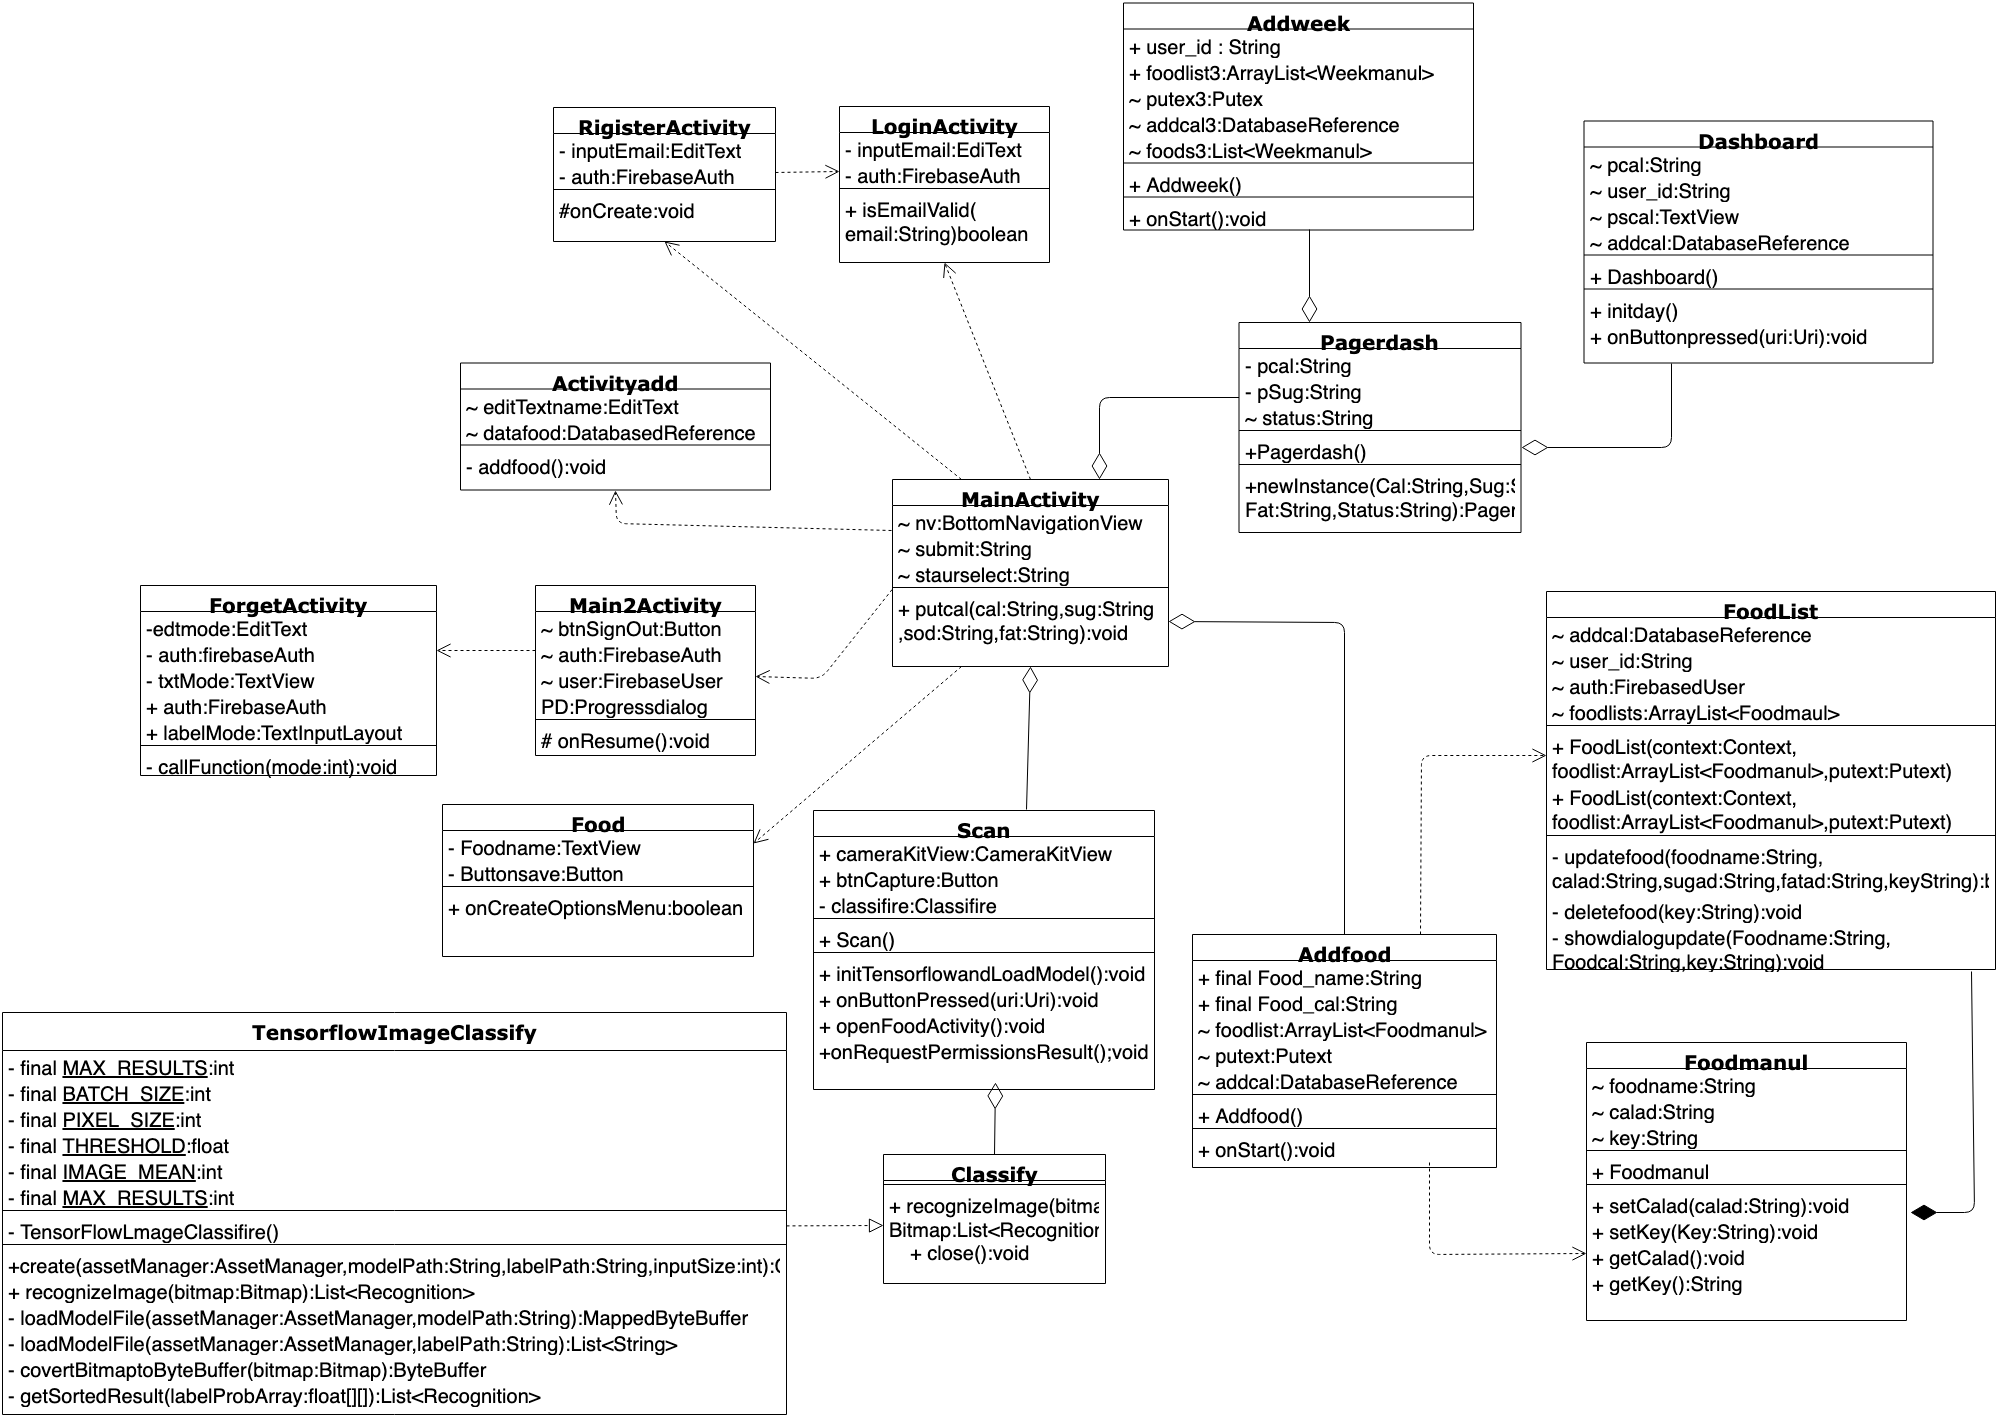
\includegraphics[width=1.1\columnwidth]{Figures/3/Class/class14.png}
		\caption{Class Diagram ของแอปพลิเคชันบีอิงเวลเนส}
		\label{Fig:MainActivity20C}
	\end{figure}


	% TABLE of class
\newpage	
	จากรูปภาพที่ \ref{Fig:MainActivity20C} สามารถอธิบายแผนภาพ Class Diagram ได้ดังนี้
	\begin{table}[H]
		\centering
		\caption{อธิบาย Class Diagram ของแอปพลิเคชันบีอิงเวลเนส}
		\label{tab:class}
		\begin{tabular}{|c|p{10cm}|}
			\hline
			\textbf{Class Diagram} & \multicolumn{1}{c|}{\textbf{คำอธิบาย}} \\ \hline
			\raisebox{-\totalheight}{LoginActivity}
			& \setstretch{1.5} {คลาส LoginActivity จะถูกเรียกใช้เมื่อสมาชิกเปิดแอพพลิเคชัน โดยวัตถุประสงค์การทำงานของคลาสนี้คือ เพื่อให้สมาชิกทำการเข้าสู่ระบบและสมัครสมาชิก } \\ \hline
			\raisebox{-\totalheight}{RigisterActivity}
			& \setstretch{1.5} {คลาส RigisterActivity จะถูกใช้งานเมื่อผู้ใช้กดปุ่ม SiGN UP โดยวัตถุประสงค์การทำงานของคลาสคือ เพื่อให้สมาชิกทำการสมัครสมาชิก} \\ \hline
			\raisebox{-\totalheight}{MainActivity}
			& \setstretch{1.5} {คลาส MainActivity เป็นคลาสหลักที่ใช้ในการทำงานของแอปพลิเคชันโดยการทำงานของคลาสนี้เน้นไปที่การเรียกใช้ Fragment โดยองค์ประกอบของคลาสนี้ประกอบไปด้วยคลาสของ Fragment ได้แก่ Pagerdash Myfood Scan} \\ \hline
			\raisebox{-\totalheight}{Main2Activiy}
			& \setstretch{1.5} {คลาส Main2Activiy เป็นคลาสที่ให้สมาชิกได้เลือกการจัดการบัญชีสมาชิก ได้แก่ เปลี่ยนอีเมล เปลี่ยนรหัสผ่าน ลบผู้ใช้ และออกจากระบบ} \\ \hline
			\raisebox{-\totalheight}{ForgetActivity}
			& \setstretch{1.5} {คลาส ForgetActivity  เป็นคลาสที่ทำการจัดการบัญชีสมาชิก ได้แก่ เปลี่ยนอีเมล เปลี่ยนรหัสผ่าน ลบผู้ใช้  } \\ \hline
			\raisebox{-\totalheight}{Activityadd}
			& \setstretch{1.5} {คลาส Activityadd  เป็นคลาสที่มีไว้สำหรับให้สมาชิกเพิ่มอาหารที่ไม่มีในระบบ } \\ \hline
			\raisebox{-\totalheight}{Food}
			& \setstretch{1.5} {คลาส Food  จะถูกใช้งานเมื่อสมาชิกทำการสแกนอาหาร โดยวัตถุประสงค์การทำงานของคลาสคือเพื่อแสดงข้อมูลอาหารที่สแกนได้ } \\ \hline

	\end{tabular}
\end{table}

\newpage
\begin{table}[H]
	\centering
	\caption{อธิบาย Class Diagram ของแอปพลิเคชันบีอิงเวลเนส(ต่อ)}
	\label{tab:class}
	\begin{tabular}{|c|p{10cm}|}
		\hline
		\textbf{Class Diagram} & \multicolumn{1}{c|}{\textbf{คำอธิบาย}} \\ \hline
		\raisebox{-\totalheight}{Pagerdash}
		& \setstretch{1.5} {คลาส Pagerdash เป็นคลาสหลักที่ใช้ในการจัดการ Tab เมนูในการเลื่อนเพื่อดูรูปแบบของข้อมูลการบริโภค} \\ \hline
		\raisebox{-\totalheight}{Addweek}
		& \setstretch{1.5} {คลาส Addweek  เป็นคลาสที่จะแสดงเมื่อสมาชิกทำการเลื่อนมาที่ Tab Week เป็นคลาสที่แสดงข้อมูลการบริโภคในรูปแบบสัปดาห์} \\ \hline
		\raisebox{-\totalheight}{Dashboard}
		& \setstretch{1.5} {คลาส Dashboard เป็นคลาสหลักที่จะถูกเรียกใช้เมื่อผู้ใช้ทำการเปิดแอปพลิเคชันหลังจากทำการเข้าสู่ระบบแล้ว โดยวัตถุประสงค์การทำงานของคลาสนี้คือ แสดงข้อมูลการบริโภคในรูปแบบวัน} \\ \hline
		\raisebox{-\totalheight}{Addfood}
		& \setstretch{1.5} {คลาส Addfood เป็นคลาสที่จะแสดงเมื่อผู้ใช้เลือกเมนู My food โดยวัตถุประสงค์การทำงานของคลาสคือแสดงรายการอาหารที่เพิ่มเข้ามา} \\ \hline
		\raisebox{-\totalheight}{FoodList}
		& \setstretch{1.5} {คลาส FoodList เป็นคลาสที่จะถูกใช้งานเมื่อคลาส Addfood ถูกใช้ โดยวัตถุประสงค์การทำงานของคลาสคือ จัดรูปแบบการแสดงรายการอาหาร} \\ \hline
		\raisebox{-\totalheight}{Foodmanul}
		& \setstretch{1.5} {คลาส Foodmanul เป็นคลาสที่กำหนดค่าต่างๆที่จำเป็นในการสร้างรายการอาหาร} \\ \hline
		\raisebox{-\totalheight}{Scan}
		& \setstretch{1.5} {คลาส Scan เป็นคลาสที่จะแสดงเมื่อผู้ใช้เลือกเมนู Scan โดยวัตถุประสงค์การทำงานของคลาสคือสแกนอาหาร} \\ \hline
		\raisebox{-\totalheight}{Classify}
		& \setstretch{1.5} {คลาส Classify เป็นคลาสที่ทำงานหลังจากสมาชิกทำการสแกน โดยวัตถุประสงค์การทำงานของคลาสคือแยกประเภทรูปภาพที่สมาชิกทำการถ่าย} \\ \hline
		\raisebox{-\totalheight}{TensorflowImageClassify}
		& \setstretch{1.5} {คลาส TensorflowImageClassify เป็นคลาสที่ทำงานร่วมกับคลาส  Classify โดยจะทำหน้าที่นำโมเดลเข้ามาเพื่อใช้ในการระบุภาพอาหารที่สมาชิกทำการถ่าย } \\ \hline
	\end{tabular}
\end{table}

\newpage
\section{Sequence Diagram}
	Sequence Diagram เป็น Diagram ที่แสดงขั้นตอนการทำงานของแต่ละ Use Case ระหว่าง Object ต่างๆ  โดย Sequence Diagram จะช่วยให้มองเห็นการทำงานของภาพรวมของระบบ ส่วนประกอบสัญลักษณ์ที่ใช้ในการเขียน Sequence Diagram 
	แสดงดังตารางที่ \ref{tab:Sequences}
	
	\begin{table}[H]
		\centering
		\caption{สัญลักษณ์ของ Sequence Diagram}
		\label{tab:Sequences}
		\begin{tabular}{| c	| p{10cm} |}
		\hline
		\textbf{สัญลักษณ์} & \multicolumn{1}{c|}{\textbf{การใช้งาน}} \\ \hline
		\raisebox{-\totalheight}{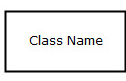
\includegraphics[width=0.17\textwidth]{Figures/table/Sequence/Sequence1}}
		& \setstretch{1.5} {Class แสดงถึงการทำงานของ Use Case ในการส่งหรือรับข้อความ แทนด้วยสัญลักษณ์สี่เหลี่ยมมีชื่อคลาสอยู่ภายใน} \\ \hline
		\raisebox{-\totalheight}{
\includegraphics[height=0.08\textheight]{Figures/table/Sequence/Sequence2}}
		& \setstretch{1.5} {Lifeline หรือเส้นอายุขัย แสดงช่วงเวลาตั้งแต่เริ่มสร้าง object ในคลาสนั้น จนกระทั่ง object นั้นถูกทำลาย สัญลักษณ์แทนด้วยเส้นประ} \\ \hline
		\raisebox{-\totalheight}{
\includegraphics[height=0.08\textheight]{Figures/table/Sequence/Sequence3}}
		& \setstretch{1.5} {Focus of control หรือจุดควบคุม เป็นจุดควบคุมที่ object ใช้ทำการส่งหรือรับข้อความ สัญลักษณ์แทนด้วยสี่เหลี่ยม} \\ \hline
		\raisebox{-\totalheight}{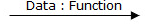
\includegraphics[width=0.3\textwidth]{Figures/table/Sequence/Sequence4}}
		& \setstretch{1.5} {Message คือ ข้อความที่รับส่งระหว่าง Object สัญลักษณ์แทนด้วยลูกศรและประกอบด้วย 2 ส่วน คือ ข้อมูล (Data) และฟังก์ชัน (Function)} \\ \hline
		\raisebox{-\totalheight}{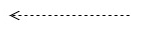
\includegraphics[width=0.3\textwidth]{Figures/table/Sequence/Sequence5}}
		& \setstretch{1.5} {Return Message เป็นข้อมูลที่ส่งกลับหลังจากทำงานเสร็จ} \\ \hline
		\raisebox{-\totalheight}{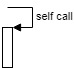
\includegraphics[height=0.08\textheight]{Figures/3/selfcall}}
		& \setstretch{1.5} {Self call เป็นการเรียกฟังชันก์การทำงานภายในตัวเอง} \\ \hline
		\raisebox{-\totalheight}{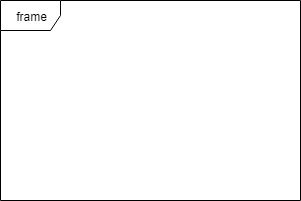
\includegraphics[height=0.1\textheight,width=0.3\textwidth]{Figures/3/frame}}
		& \setstretch{1.5} {สร้างกรอบการทำงานของโปรแกรม เพื่อให้รู้ขอบเขตของการทำงานเช่น ลูป(loop)} \\ \hline
		\end{tabular}
	\end{table}
%
%	Sequence Diagram ที่ใช้อธิบายการทำงานของระบบกองทุนเงินให้กู้ยืมเพื่อการศึกษา คณะวิทยสศาสตร์ มหาวิทยาลัยอุบลราชธานี มีรายละเอียดดังต่อไปนี้

\newpage
	\begin{landscape}
	\begin{figure}[H]
		\centering
		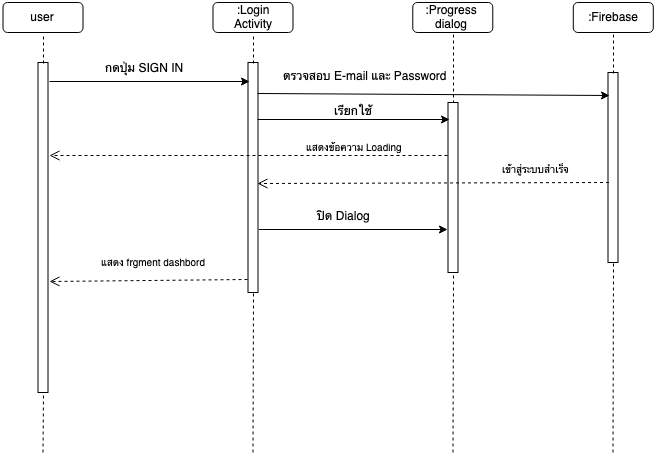
\includegraphics[width=0.8\columnwidth]
		{Figures/3/Sequence/sqlogin.png}
		\caption{Sequence Diagram การเข้าสู่ระบบ}
		\label{Fig:Sequence-login}
	\end{figure}
  \end{landscape}

		\label{Fig:Sequence-login}
		จากภาพที่ \ref{Fig:Sequence-login} สามารถอธิบายแผนภาพ Sequence Diagram การเข้าสู่ระบบ ได้ดังนี้ เมื่อ
	สมาชิกกดปุ่ม SIGN IN  ที่คลาส LoginActivity จะทำการตรวจสอบ E-mail และ Password โดยส่งไปที่ Firebase ในขณะเดียวกันก็จะเรียก Progess dialog แสดงข้อความไปยังสมาชิกว่า Loading 
	 เมื่อเข้าสู่ระบบสำเร็จจะทำการปิด Dialog แล้วแสดง fragment dashbord ที่สมาชิก
	\begin{sidewaysfigure}
	\begin{figure}[H]
		\centering
		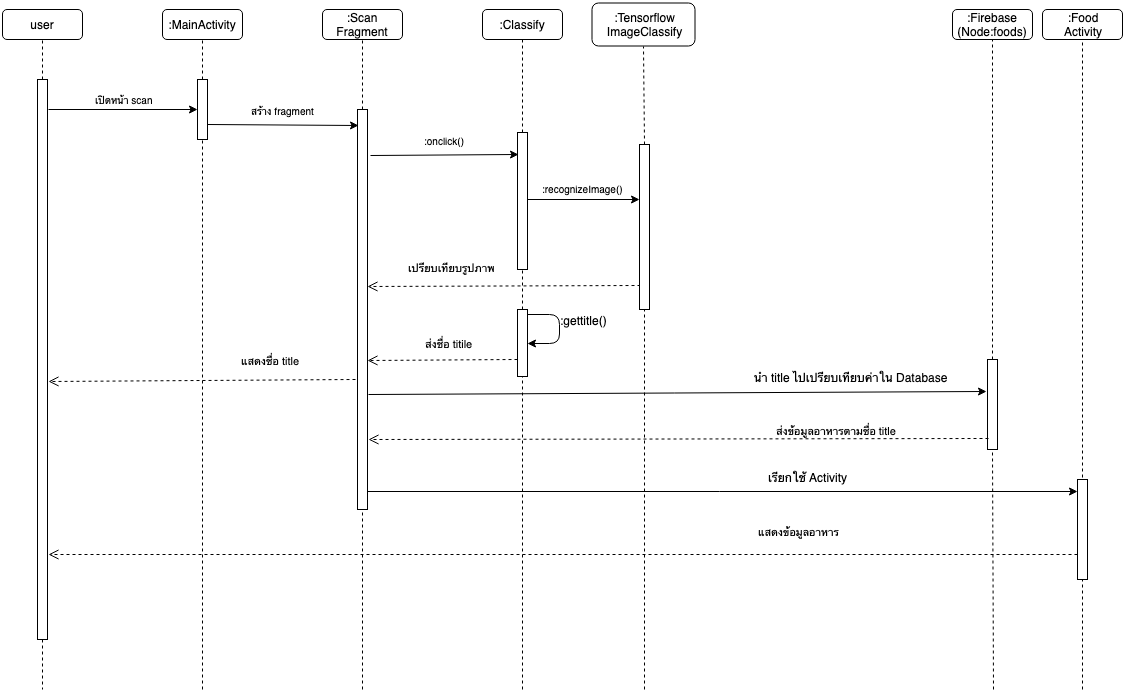
\includegraphics[width=0.8\columnwidth]
		{Figures/3/Sequence/sqscannew1.png}
		\caption{Sequence Diagram การสแกน}
		\label{Fig:Sequence-scan}
	\end{figure}
	\end{sidewaysfigure}
	\newpage
	จากภาพที่ \ref{Fig:Sequence-scan} สามารถอธิบายแผนภาพ Sequence Diagram การสแกน ได้ดังนี้ เมื่อสมาชิกทำการเปิดหน้าสแกน คลาส MainActivity จะทำการสร้่าง Fragent Scan ขึ้นมาและเมื่อสมาชิกกดปุ่ม Scan ฟังก์ชัน Onclick() จะทำการส่งข้อมูลไปยังคลาส Classify จากนั้นคลาส Classify 
	จะทำการ :recognizeImage() แล้วให้คลาส TensorflowImageClassify ทำการเปรียบเทียบรูปภาพ หลังจากการเปรียบเทียบรูปภาพแล้วที่ Fragment Scan จะใช้เมธอด getitile() แล้วส่งชื่อ title ที่ได้มาแสดงให้หับสมาชิก แล้วนำ title ที่แสดงไปเปรียบกับค่าใน Firebased ที่โหนด foods แล้วส่งข้อมูลหารที่ตรงกันกับ title 
	จากนั้นเรียกใช้ FoodActivity ที่หแสดงข้อมูลอาหารให้กับสมาชิก
 
	\begin{sidewaysfigure}
	\begin{figure}[H]
		\centering
		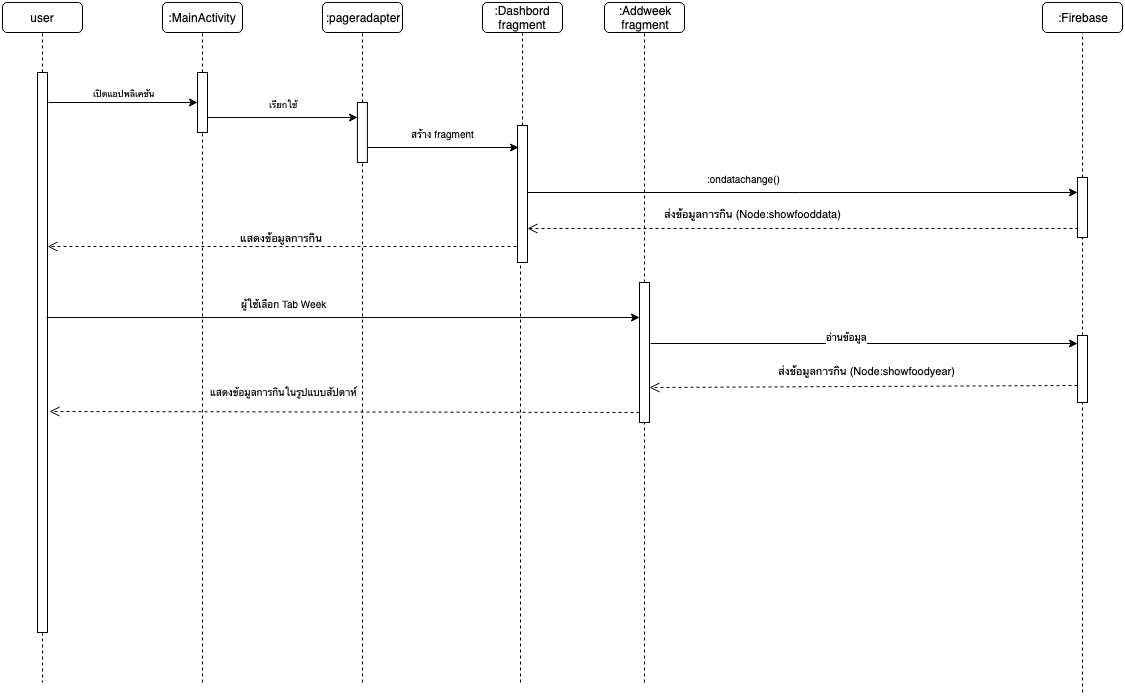
\includegraphics[width=1\columnwidth]
		{Figures/3/Sequence/sqtabnew.png}
		\caption{Sequence Diagram ดูข้อมูลการบริโภครูปแบบวัน สัปดาห์และเดือน}
		\label{Fig:Sequence-sqtab}
	\end{figure}
	\end{sidewaysfigure}
	\newpage
	จากภาพที่ \ref{Fig:Sequence-sqtab} สามารถอธิบายแผนภาพ Sequence Diagram ดูข้อมูลการบริโภครูปแบบวัน สัปดาห์และเดือน ได้ดังนี้ เมื่อสมาชิกเปิดแอปพลิเคชันคลาส MainActivity จะเรียกใช้ Pagerdash  
	ซึ่งประกอบไปด้วย Fragment ดังนี้  Dashboard Addweek และ Addmonth 	จากนั้นแต่ละ Fragment จะทำเมธอด ondatachange() 
	ด้วยการอ่านข้อมูลที่ Firebase โหนด Showfooddata Showfoodyear และ ShowfoodMonth ตาม Tab ที่ผู้ใช้เลือกดู

	\begin{sidewaysfigure}
	\begin{figure}[H]
		\centering
		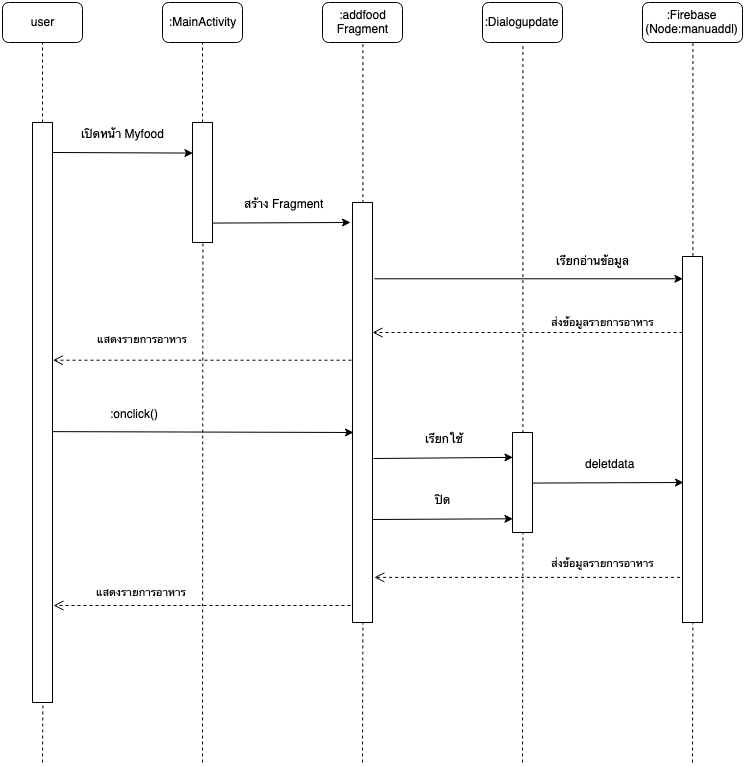
\includegraphics[width=0.6\columnwidth]
		{Figures/3/Sequence/sqdelete.png}
		\caption{Sequence Diagram ลบอาหารที่เพิ่ม}
		\label{Fig:Sequence-delete}
	\end{figure}
	\end{sidewaysfigure}
	\newpage
	จากภาพที่ \ref{Fig:Sequence-delete} สามารถอธิบายแผนภาพ Sequence Diagram ลบอาหารที่เพิ่ม ได้ดังนี้ เมื่อผู้ใช้เปิดหน้า Myfood คลาส MainActivity จะทำการสร้าง Fragment addfood  จากนั้นจะทำการอ่านข้อมูลที่ Firebase มาแสดงรายการอาหารที่สมาชิก และเมื่อผู้ใช้กดที่รายการอาหาร  Fragment addfood  จะเรียกใช้ Dialogupdate แล้วลบข้อมูลออก หลังจากที่ลบข้อมูลแล้วก็จะทำการปิด Dialogupdate 
	จากนั้น Firebase จะส่งข้อมูลรายการอาหารที่มีอยู่มา แสดงที่สมาชิกอีกครั้ง
	\newpage	

	
\section{โครงสร้างฐานข้อมูลไฟร์เบส(Firebase Database Stucture)}
Firebase Database นั้นเป็น Database แบบ NoSQL และเป็น JSON database ที่มีโครงสร้างที่เป็น Key และ Value จัดเก็บข้อมูลในลักษณะโหนด หากต้องการเรียกงานจะเรียกใช้โดย
การท่องไปยังโหนดที่ต้องการ ส่วนประกอบสัญลักษณ์ที่ใช้ในการเขียนโครงสร้างฐานข้อมูลแบบ Firebase
แสดงดังตารางที่ \ref{tab:DB}

\begin{table}[H]
	\centering
	\caption{สัญลักษณ์ของโครงสร้างฐานข้อมูลแบบ Firebase}
	\label{tab:DB}
	\begin{tabular}{| c	| p{10cm} |}
		\hline
		\textbf{สัญลักษณ์} & \multicolumn{1}{c|}{\textbf{คำอธิบาย}} \\ \hline
		\raisebox{-\totalheight}{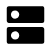
\includegraphics[width=0.1\textwidth]{Figures/3/DB/dbroot}}
		& \setstretch{1.5} {Database เป็นการเรียกชื่อแทนรูทโหนด(Root Node)บนสุดที่ใช้ในการเก็บข้อมูล} \\ \hline
		\raisebox{-\totalheight}{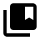
\includegraphics[width=0.1\textwidth]{Figures/3/DB/dbcollection}}
		& \setstretch{1.5} {Key  เป็นโหนด(Node) ที่รองลงมาจากรูทโหนด ซึ่งประกอบไปด้วย KeyและValue } \\ \hline
	\end{tabular}
\end{table}
	\begin{figure}[H]
	\centering
	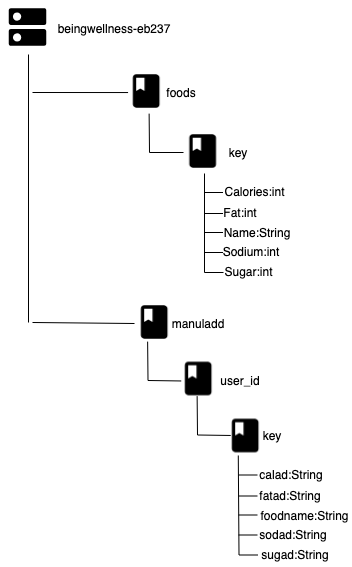
\includegraphics[width=0.7\columnwidth]
	{Figures/3/DB/firebase.png}
	\caption{โครงสร้างฐานข้อมูลแบบ Firebase}
	\label{Fig:DB1}
	\end{figure}

	\begin{figure}[H]
	\centering
	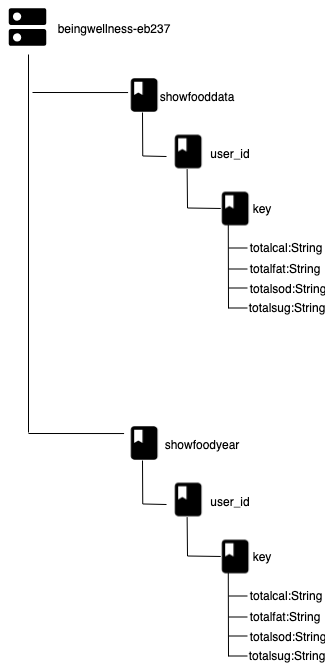
\includegraphics[width=0.6\columnwidth]
	{Figures/3/DB/firebase2.png}
	\caption{โครงสร้างฐานข้อมูลแบบ Firebase(ต่อ)}
	\label{Fig:DB2}
\end{figure}
	\begin{figure}[H]
	\centering
	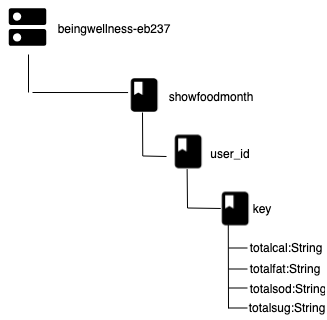
\includegraphics[width=0.7\columnwidth]
	{Figures/3/DB/showfoodmonth.png}
	\caption{โครงสร้างฐานข้อมูลแบบ Firebase(ต่อ)}
	\label{Fig:DB3}
\end{figure}
	

\newpage
จากรูที่ \ref{Fig:DB1}-\ref{Fig:DB3} สามารถอธิบายโครงสร้างของข้อมูลได้ดังนี้
\begin{figure}[H]
\centering
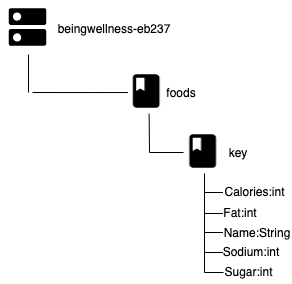
\includegraphics[width=0.6\columnwidth]
{Figures/3/DB/nodefood.png}
\caption{โหนดเก็บข้อมูลประกาศ}
\label{Fig:DB4}
\end{figure}
\begin{table}[H]
	\centering
	\caption{อธิบายโหนดที่ใช้เก็บข้อมูลอาหาร}
	\label{my-label1}
	\begin{tabular}{|c|p{10cm}|}
		\hline
		\multicolumn{1}{|c|}{\textbf{Key}} & \multicolumn{1}{c|}{\textbf{คำอธิบาย}} \\ \hline
		foods & โหนดสำหรับเก็บข้อมูลอาหารในระบบทั้งหมก \\ \hline
		Key &  โหนดสำหรับเก็บคีย์ของอาหาร \\ \hline
		Calories & สำหรับเก็บแคลลอรี่ของอาหาร \\ \hline
		Fat & สำหรับเก็บค่าไขมันของอาหาร  \\ \hline
		Name &  สำหรับเก็บชื่อของอาหาร \\ \hline
		Sodium &  สำหรับเก็บค่าโซเดียมของอาหาร \\ \hline
		Sugar & สำหรับเก็บค่าน้ำตาลของอาหาร \\ \hline
		\end{tabular}
\end{table}

\newpage
\begin{figure}[H]
	\centering
	\includegraphics[width=0.7\columnwidth]
	{Figures/3/DB/manuladd.png}
	\caption{โหนดเก็บข้อมูลอาหารที่สมาชิกเพิ่มเข้ามา}
	\label{Fig:DB4}
\end{figure}
\begin{table}[H]
	\centering
	\caption{อธิบายโหนดเก็บข้อมูลอาหารที่สมาชิกเพิ่มเข้ามา}
	\label{my-label1}
	\begin{tabular}{|c|p{10cm}|}
		\hline
		\multicolumn{1}{|c|}{\textbf{Key}} & \multicolumn{1}{c|}{\textbf{คำอธิบาย}} \\ \hline
		manuladd & โหนดสำหรับเก็บข้อมูลอาหารที่สมาชิกเพิ่มเข้ามาทั้งหมด \\ \hline
		user\_id &  โหนดสำหรับเก็บข้อมูลอาหารที่เพิ่มเข้าของสมาชิกแต่ละคน\\ \hline
		key & โหนดสำหรับเก็บ ID ของอาหารที่สมาชิกเพิ่มเข้ามา \\ \hline
		calad & สำหรับเก็บแคลลอรี่ของอาหารที่ผู้ใช้เพิ่มเข้ามา \\ \hline
		fatad & สำหรับเก็บแคลลอรี่ของอาหารที่ผู้ใช้เพิ่มเข้ามา\\ \hline
		foodname & สำหรับเก็บแคลลอรี่ของอาหารที่ผู้ใช้เพิ่มเข้ามา\\ \hline
		sodad & สำหรับเก็บแคลลอรี่ของอาหารที่ผู้ใช้เพิ่มเข้ามา\\ \hline
		sugad & สำหรับเก็บแคลลอรี่ของอาหารที่ผู้ใช้เพิ่มเข้ามา\\ \hline

	\end{tabular}
\end{table}

\newpage
\begin{figure}[H]
	\centering
	\includegraphics[width=0.6\columnwidth]
	{Figures/3/DB/showfooddata.png}
	\caption{โหนดเก็บข้อมูลการบริโภคในรูปแบบวัน}
	\label{Fig:DB4}
\end{figure}
\begin{table}[H]
	\centering
	\caption{อธิบายโหนดเก็บข้อมูลการบริโภคในรูปแบบวัน}
	\label{my-label1}
	\begin{tabular}{|c|p{10cm}|}
		\hline
		\multicolumn{1}{|c|}{\textbf{Key}} & \multicolumn{1}{c|}{\textbf{คำอธิบาย}} \\ \hline
		showfooddata & โหนดสำหรับเก็บข้อมูลการบริโภคในรูปแบบวันทั้งหมด\\ \hline
		User\_id &  สำหรับเก็บข้อมูลการบริโภคในรูปแบบวันของสมาชิกแต่ละคน \\ \hline
		Key & สำหรับเก็บข้อมูลวันที่ \\ \hline
		totalcal & สำหรับเก็บข้อมูลแคลลอรี่ในรูปแบบวัน \\ \hline
		totalfat & สำหรับเก็บข้อมูลไขมันรี่ในรูปแบบวัน \\ \hline
		totalsod & สำหรับเก็บข้อมูลโซเดียมในรูปแบบวัน\\ \hline
		totalsug & สำหรับเก็บข้อมูลน้ำตาลในรูปแบบวัน\\ \hline
	
	\end{tabular}
\end{table}

\newpage
\begin{figure}[H]
	\centering
	\includegraphics[width=0.6\columnwidth]
	{Figures/3/DB/showfoodyear.png}
	\caption{โหนดเก็บข้อมูลการบริโภคในรูปแบบสัปดาห์}
	\label{Fig:DB4}
\end{figure}
\begin{table}[H]
	\centering
	\caption{อธิบายโหนดที่เก็บข้อมูลการบริโภคในรูปแบบสัปดาห์}
	\label{my-label1}
	\begin{tabular}{|c|p{10cm}|}
		\hline
		\multicolumn{1}{|c|}{\textbf{Key}} & \multicolumn{1}{c|}{\textbf{คำอธิบาย}} \\ \hline
		showfoodyear & โหนดสำหรับเก็บข้อมูลการบริโภคในรูปแบบสัปดาห์ทั้งหมด\\ \hline
		User\_id &  สำหรับเก็บข้อมูลการบริโภคในรูปแบบสัปดาห์ของสมาชิกแต่ละคน \\ \hline
		Key & สำหรับเก็บข้อมูลสัปดาห์\\ \hline
		totalcal & สำหรับเก็บข้อมูลแคลลอรี่ในรูปแบบสัปดาห์ \\ \hline
		totalfat & สำหรับเก็บข้อมูลไขมันรี่ในรูปแบบสัปดาห์ \\ \hline
		totalsod & สำหรับเก็บข้อมูลโซเดียมในรูปแบบสัปดาห์\\ \hline
		totalsug & สำหรับเก็บข้อมูลน้ำตาลในรูปแบบสัปดาห์\\ \hline
	\end{tabular}
\end{table}

\newpage
\begin{figure}[H]
	\centering
	\includegraphics[width=0.6\columnwidth]
	{Figures/3/DB/showfoodmonth.png}
	\caption{โหนดเก็บข้อมูลการบริโภคในรูปแบบเดือน}
	\label{Fig:DB4}
\end{figure}
\begin{table}[H]
	\centering
	\caption{อธิบายโหนดที่เก็บข้อมูลการบริโภคในรูปแบบเดือน}
	\label{my-label1}
	\begin{tabular}{|c|p{10cm}|}
		\hline
		\multicolumn{1}{|c|}{\textbf{Key}} & \multicolumn{1}{c|}{\textbf{คำอธิบาย}} \\ \hline
		showfoodyear & โหนดสำหรับเก็บข้อมูลการบริโภคในรูปแบบเดือนทั้งหมด\\ \hline
		User\_id &  สำหรับเก็บข้อมูลการบริโภคในรูปแบบเดือนของสมาชิกแต่ละคน \\ \hline
		Key & สำหรับเก็บข้อมูลเดือน\\ \hline
		totalcal & สำหรับเก็บข้อมูลแคลลอรี่ในรูปแบบเดือน \\ \hline
		totalfat & สำหรับเก็บข้อมูลไขมันรี่ในรูปแบบเดือน \\ \hline
		totalsod & สำหรับเก็บข้อมูลโซเดียมในรูปแบบเดือน\\ \hline
		totalsug & สำหรับเก็บข้อมูลน้ำตาลในรูปแบบเดือน\\ \hline
	\end{tabular}
\end{table}
\newpage
	
\section{ขั้นตอนการเตรียมข้อมูลและการสร้างโมเดล}
ในขั้นตอนการเตรียมข้อมูลและการสร้างโมเดลเป็นหนึ่งในขั้นตอนที่สำคัญของแอปพลิเคชัน เนื่องจากการเตรียมข้อมูลที่ดีจะส่งผลถึงความถูกต้องและแม่นยำในการ
สแกนอาหาร ในการฝึกฝนได้เลือกใช้เทคโนโลยี Tensorflow Lite เป็นเครื่องมือหลัก เพราะ Tensorflow Lite ได้ใช้เทคโนโลยีโครงข่ายประสาทเทียมเพื่อเพิ่มความ
ถูกต้องและความแม่นยำในการสแกนอีกทั้งยังสนับสนุนการนำไปใช้ร่วมกับระบบปฏิบัติการแอนดรอยด์ ซึ่งขั้นตอนการเตรียมข้อมูลมีดังต่อไปนี้  
% \begin{enumerate}
% 	\item  การเก็บข้อมูลรูปอาหาร
% 	\item  การตั้งค่าขนาดรูปและการใช้รูปแบบการจำแนก
% 	\item  การสร้างโมเดลด้วย Tensorflow Lite 
% 	\item  การแปลงไฟล์ PB ไปเป็น lite 
% \end{enumerate}

\subsection{การเก็บข้อมูลรูปอาหาร}
การสร้างโมเดลของระบบ ได้ใช้ภาพสินค้าที่แตกต่างกันจำนวน 50 รูป ซึ่งเป็นสินค้าที่ขายดีที่สุดใน  เซเว่น-อีเลฟเว่น 
				\begin{figure}[H]
								\centering
								\includegraphics[width=0.8\textwidth]{Figures/3/ten/prepic.png}
								\caption{การเก็บข้อมูลภาพอาหาร}
								\label{Fig:picfood}
							\end{figure}
							จากภาพที่ \ref{Fig:picfood} สามารถอธิบายได้ดังนี้ินค้าแต่ละชนิดจะใช้ภาพจำนวน 100 ภาพในการฝึกฝน 
	

		\subsection{การตั้งค่าขนาดภาพและการใช้รูปแบบการจำแนก}
							ในขั้นตอนนี้จะทำการตั้งค่าขนาดภาพและเลือกใช้รูปแบบการจำแนก Mobilenet\_v1 โดยใช้คำสั่งเพื่อรันดังภาพที่ \ref{Fig:mobile}
			

\begin{figure}[H]
{\setstretch{1.0}\begin{lstlisting}
IMAGE_SIZE=224                  
ARCHITECTURE="mobilenet_v1_1.0_${IMAGE_SIZE}"
\end{lstlisting}}
\caption{คำสั่งการตั้งค่าขนาดภาพและการใช้รูปแบบการจำแนก}
\label{Fig:mobile}
\end{figure}
จากภาพที่ \ref{Fig:mobile} คำสั่งการตั้งค่าขนาดภาพและการใช้รูปแบบการจำแนก สามารถอธิบายการทำงานได้ดังนี้
\begin{itemize}[label={--}]
	\item บรรทัดที่  1	     เป็นการตั้งค่าขนาดของภาพเพื่ิอให้ภาพมีขนาดเท่ากัน
	\item บรรทัดที่  2 	     เป็นการเลือกใช้รูปแบบการจำแนกเพื่อทำการฝึกฝน  
\end{itemize}


	\subsection{การสร้างโมเดลด้วย Tensorflow Lite}
							ในขั้นตอนนี้จะทำการตั้งค่าขนาดภาพและเลือกใช้รูปแบบการจำแนก Mobilenet\_v1 โดยใช้คำสั่งเพื่อรันดังภาพที่ \ref{Fig:model}

\begin{figure}[H]
{\setstretch{1.0}\begin{lstlisting}
sudo python -m scripts.retrain \
--bottleneck_dir=tf_files/bottlenecks \
--how_many_training_steps=40000 \
--model_dir=tf_files/models/ \
--summaries_dir=tf_files/training_summaries/"${ARCHITECTURE}" \
--output_graph=tf_files/retrained_graph.pb \
--output_labels=tf_files/retrained_labels.txt \
--architecture="${ARCHITECTURE}" \
--image_dir=tf_files/test

\end{lstlisting}}
\caption{คำสั่งการตั้งค่าขนาดภาพและการใช้รูปแบบการจำแนก}
\label{Fig:model}
\end{figure}
\newpage




จากภาพที่ \ref{Fig:model} โครงสร้างขคำสั่งการตั้งค่าขนาดภาพและการใช้รูปแบบการจำแนกสามารถอธิบายการทำงานได้ดังนี้
\begin{itemize}[label={--}]
\item บรรทัดที่  1	     เป็นคำสั่งรันสคริปที่ทาง Google ได้ทำไว้
\item บรรทัดที่  2 	     เป็นคำสั่งสำหรับการเข้ารหัสรูปภาพ
\item บรรทัดที่  3       เป็นคำสั่งที่ระบุจำนวนของการฝึกฝน 
\item บรรทัดที่  4       เป็นคำสั่งระบุที่อยู่ของโมเดล 
\item บรรทัดที่  5       เป็นคำสั่งระบุที่อยู่ในการจัดเก็บผลลัพธ์จากการฝึกฝน
\item บรรทัดที่  6       เป็นคำสั่งระบุที่อยู่ในการ Export ไฟล์ retrained\_graph.PB 
\item บรรทัดที่  7       เป็นคำสั่งระบุที่อยู่ในการ Export ไฟล์ retrained\_labels.text 
\item บรรทัดที่  8       เป็นคำสั่งใช้งานรูปแบบการจำแนก
\item บรรทัดที่  9       เป็นคำสั่งระบุที่อยู่ของรูปภาพ
\end{itemize}
\subsection{การแปลไฟล์ PB ไปเป็น lite}
ในขั้นตอนนี้จะแปลงไฟล์ PB ไปเป็น lite เพื่อนำไปใช้กับแอนดรอย์แอปพลิเคชัน โดยใช้คำสั่งเพื่อรันดังภาพที่ \ref{Fig:convert}

\begin{figure}[H]
{\setstretch{1.0}\begin{lstlisting}
IMAGE_SIZE=224
tflite_convert \
--graph_def_file=tf_files/retrained_graph.pb \
--output_file=tf_files/optimized_graph.lite \
\end{lstlisting}}
\caption{คำสั่งในการแปลงไฟล์ PB ไปเป็น lite }
\label{Fig:convert}
\end{figure}
จากภาพที่ \ref{Fig:convert} คำสั่งการแปลงไฟล์ PB ไปเป็น lite สามารถอธิบายการทำงานได้ดังนี้
\begin{itemize}[label={--}]
\item บรรทัดที่  1	     เป็นการเรียกใช้สคริปสำหรับการแปลงไฟล์
\item บรรทัดที่  2 	     เป็นคำสั่งระบุที่อยู่ของไฟล์ PB 
\item บรรทัดที่  3       เป็นคำสั่งระบุที่จัดเก็บไฟล์ lite  
\end{itemize}



								
			
\chapter{การพัฒนาระบบ}
หลังจากที่ได้มีการเตรียมความพร้อมสำหรับการพัฒนาในด้านต่าง ไม่ว่าจะเป็นที่มาและความสำคัญของปัญหา เทคโนโลยีที่มีความเหมาะสมกับระบบ และการออกแบบระบบการทำงานรวมไปถึงโครงสร้างของข้อมูล ในบทนี้จะเป็นการพูดถึงการสร้างระบบที่ได้มีการออกแบบไว้ในบทที่แล้วจะถูกนำเสนอในบทนี้ ซึ่งจะอธิบายถึงตัวอย่างการทำงานของแอปพลิเคชันดังนี้
		\section{โครงสร้างของการสร้างหน้า MainActivity}
		\begin{figure}[H]
			{\setstretch{1.0}\begin{lstlisting}
Scan scan;
Addfood addfood;
Dashboard dash;
Pagerdash pagerdash;
BottomNavigationView nv;
				\end{lstlisting}}
			\caption{ตัวแปรในคลาส MainActivity}
			\label{Fig:MainActivity}
		\end{figure}
		จากภาพที่ \ref{Fig:MainActivity} ตัวแปรที่ประกาศขึ้นเพื่อใช้ในการทำงานของคลาส MainActivity สามารถอธิบายได้ดังนี้
		\begin{itemize}[label={--}]
			\item บรรทัดที่ 1 ตัวแปร scan ใช้แสดงผลหน้าสแกน
			\item บรรทัดที่ 2 ตัวแปร addfood ใช้แสดงผลหน้าจอเพิ่มอาหารโดยสมาชิก  
			\item บรรทัดที่ 3 ตัวแปร dash ใส้แสดงผลหน้าจอแดชบอร์ด
			\item บรรทัดที่ 4 ตัวแปร pagerdash เป็นตัวแปลงหน้าจอเมื่อผู้ใช้เลือก Tab Week หรือ Tab Month
			\item บรรทัดที่ 5 ตัวแปร nv เป็นที่เก็บเมนู Scan และ Myfood มีไว้ให้สมาชิกเลือก
		
		\end{itemize}

		

		\begin{figure}[H]
			{\setstretch{1.0}\begin{lstlisting}
        @Override
 public boolean onNavigationItemSelected(@NonNull MenuItem menuItem) {
     switch (menuItem.getItemId()) {
         case R.id.cam:
             if (staurselect != "scan") {
                 ft = getSupportFragmentManager().beginTransaction().replace(R.id.Framefag, scan);
                 ft.commit();
                 staurselect = "scan";
             }
             break;
         case R.id.dash:
             if (staurselect != "dashbord" ) {
                 Calories = Sugar = Sodium = Fat = submit = null;
                 ft = getSupportFragmentManager().beginTransaction().replace(R.id.Framefag, new Pagerdash().newInstance(Calories,Sugar,Sodium,Fat,submit));
                 ft.commit();
                 staurselect = "dashbord";
             }
             break;
         case  R.id.cart:
             if (staurselect != "Addfood"){
                 ft = getSupportFragmentManager().beginTransaction().replace(R.id.Framefag, addfood );
                 ft.commit();
                 staurselect = "Addfood";
             }
             break;
     }
     return true;
 }

				\end{lstlisting}}
			\caption{โค้ดส่วนที่ใช้ในการสร้างเมนูนำทางหลักภายในคลาส MainActivity}
			\label{Fig:MainActivity2}
		\end{figure}
\newpage
		จากภาพที่ \ref{Fig:MainActivity2} สามารถอธิบายการทำงานโค้ดส่วนที่ใช้เมนูนำทางหลักภายในคลาส MainActivity ได้ดังนี้
		\begin{itemize}[label={--}]
			\item บรรทัดที่ 1     เป็นการเพิ่มการดักจับอีเวนต์ (Event) เพื่อสลับหน้าจอการแสดงผลที่เกิดขึ้นเมื่อผู้ใช้กดที่เมนูนำทาง
			\item บรรทัดที่ 2-3   เป็นการเรียกใช้เมธอดชันจากคลาสที่ extends มา
			\item บรรทัดที่ 4     เป็นการรับ ID 
			\item บรรทัดที่ 5    	เป็นการระบุ ID ไปยังไอคอน cam ที่ไฟล์ xml
			\item บรรทัดที่ 6-9 	เป็นการแสดงหน้าจอสแกนและป้องกันการกดหน้าสแกนซ้ำ
			\item บรรทัดที่ 10 		เป็นการหยุดการทำงานของ case เพื่อไม่ให้ทำงานต่อเนื่อง 
			\item บรรทัดที่ 11	  เป็นการระบุไปยังไอคอน dash ที่ไฟล์ xml
			\item บรรทัดที่ 12-17 เป็นการแสดงหน้าจอแดชบอร์ดและป้องกันการกดหน้าสแกนซ้ำ
			\item บรรทัดที่ 18    เป็นการหยุดการทำงานของ case เพื่อไม่ให้ทำงานต่อเนื่อง 
			\item บรรทัดที่ 19    เป็นการระบุ ID ไปยังไอคอน cart ที่ไฟล์ xml
			\item บรรทัดที่ 20-24 เป็นการแสดงหน้าจอเพิ่มอาหารและป้องกันการกดหน้าสแกนซ้ำ
			\item บรรทัดที่ 25-29 เป็นการหยุดการทำงานของ case เพื่อไม่ให้ทำงานต่อเนื่องและจบการทำงานของเมนูนำทาง 
		\end{itemize}
	
	\section{โครงสร้างของการสร้างหน้า Main2Activity}
	\begin{figure}[H]
		{\setstretch{1.0}\begin{lstlisting}
Button btnSignOut;
FirebaseAuth auth;
FirebaseUser user;
ProgressDialog PD;
	
			\end{lstlisting}}
		\caption{ตัวแปรในคลาส Main2Activity}
		\label{Fig:Main2Activity}
	\end{figure}
	\newpage
	จากภาพที่ \ref{Fig:Main2Activity} ตัวแปรที่ประกาศขึ้นเพื่อใช้ในการทำงานของคลาส FeedFragment สามารถอธิบายได้ดังนี้
	\begin{itemize}[label={--}]
		\item บรรทัดที่ 1 ตัวแปร btnSignOut ใช้ในการแสดงข้อมูลลิสต์รายการข่าวสาร
		\item บรรทัดที่ 2 ตัวแปร auth ใช้จัดเก็บและยืนตัวตนของสมาชิก
		\item บรรทัดที่ 3 ตัวแปร user ใช้จัดการข้อมูลของสมาชิก
		\item บรรทัดที่ 4 ตัวแปร pd ใช้สำหรับเป็นแจ้งเตือน
	\end{itemize}
	\begin{figure}[H]
		{\setstretch{1.0}\begin{lstlisting}
btnSignOut.setOnClickListener(new View.OnClickListener() {
    @Override
    public void onClick(View view) {
        auth.signOut();
        Intent intent = new Intent(Main2Activity.this, LoginActivity.class);
        startActivity(intent);
        finish();
        MainActivity.activityMain.finish();
    }
});

findViewById(R.id.change_password_button).setOnClickListener(new View.OnClickListener() {
    @Override
    public void onClick(View view) {
        startActivity(new Intent(getApplicationContext(), ForgetActivity.class).putExtra("Mode", 1));
    }
});

findViewById(R.id.change_email_button).setOnClickListener(new View.OnClickListener() {		@Override            		public void onClick(View view) {
        startActivity(new Intent(getApplicationContext(), ForgetActivity.class).putExtra("Mode", 2));
    }
});
findViewById(R.id.delete_user_button).setOnClickListener(new View.OnClickListener() {
 @Override            
 public void onClick(View view) {
                startActivity(new Intent(getApplicationContext(), ForgetActivity.class).putExtra("Mode", 3));
            }
        });
    }
			\end{lstlisting}}
		\caption{โค้ดส่วนที่ใช้ในการสร้างเมนูนำทางหลักภายในคลาส Main2Activity}
		\label{Fig:Main2Activity2}
	\end{figure}
	จากภาพที่ \ref{Fig:Main2Activity2} โค้ดส่วนที่ใช้ในการสร้างเมนูนำทางหลักภายในคลาส Main2Activity สามารถอธิบายได้ดังนี้
	\begin{itemize}[label={--}]
		\item บรรทัดที่ 1 ทำหน้าที่ดักจับอีเวนต์ดักจักเมื่อผู้ใช้ทำการกดปุ่ม SIGN OUT
		\item บรรทัดที่ 2-10  เป็นการทำงานเมื่อผู้ใช้กดปุ่ม SIGN OUT  จะทำการออกจากระบบและทำลาย Activity ทั้งหมด
		\item บรรทัดที่ 12-17 เป็นการทำงานเมื่อผู้ใช้กดปุ่ม CHANGE PASSWORD ระบบจะทำการส่งค่า Mode 1
		\item บรรทัดที่ 19-22 เป็นการทำงานเมื่อผู้ใช้กดปุ่ม CHANGE Email ระบบจะทำการส่งค่า Mode 2
		\item บรรทัดที่ 23-29 เป็นการทำงานเมื่อผู้ใช้กดปุ่ม Delete User ระบบจะทำการส่งค่า Mode 3
	\end{itemize}
	
	\section{โครงสร้างของการสร้างหน้า DashboardFragment}
	\begin{figure}[H]
		{\setstretch{1.0}\begin{lstlisting}
List<PieEntry> entries;
PieChart pieChart;
public   static ObjectAnimator progresanimator3, progresanimator2, progresanimator1;
public   static ProgressBar progressBar3, progressBar2, progressBar1;
	\end{lstlisting}}
		\caption{ตัวแปรในคลาส DashboardFragment}
		\label{Fig:DashboardFragment}
	\end{figure}
	จากภาพที่ \ref{Fig:DashboardFragment} ตัวแปรที่ประกาศขึ้นเพื่อใช้ในการทำงานของคลาส DashboardFragment สามารถอธิบายได้ดังนี้
	\begin{itemize}[label={--}]
		\item บรรทัดที่ 1 ตัวแปร entries ใช้สำหรับเก็บข้อมูลลงใน chart
		\item บรรทัดที่ 2 ตัวแปร ObjectAnimator progresanimator3, progresanimator2, progresanimator1 ใช้ตั้งค่าทำให้ chart เคล่ือนไหว
		\item บรรทัดที่ 3 ตัวแปร ProgressBar progressBar3, progressBar2, progressBar1 ใช้ตั้งค่า ProgressBar
	\end{itemize}
	\begin{figure}[H]
		{\setstretch{1.0}\begin{lstlisting}
Date currentTime = Calendar.getInstance().getTime();
SimpleDateFormat df = new SimpleDateFormat("dd-MM-yyyy");
SimpleDateFormat simplemonth = new SimpleDateFormat("MMM-yyyy", Locale.ENGLISH);
SimpleDateFormat simpleyear = new SimpleDateFormat("ww-YYYY");
final String month2 = simplemonth.format(currentTime);
final String year = simpleyear.format(currentTime);
final String date = df.format(currentTime);
	
			\end{lstlisting}}
		\caption{โค้ดส่วนที่ใช้ในการสร้างโหนดวัน สัปดาห์และเดือนภายในคลาส Dashbord}
		\label{Fig:Dashbord}
	\end{figure}
	จากภาพที่ \ref{Fig:Dashbord} โค้ดส่วนที่ใช้ในการสร้างเมนูนำทางหลักภายในคลาส Main2Activity สามารถอธิบายได้ดังนี้
	\begin{itemize}[label={--}]
		\item บรรทัดที่ 1  เป็นการดึงวันที่จากสมาร์ทโฟนมาใช้งาน
		\item บรรทัดที่ 2  เป็นการเลือกรูปแบบวันที่ให้อยู่ในรูปแบบ วัน
		\item บรรทัดที่ 3  เป็นการเลือกรูปแบบวันที่ให้อยู่ในรูปแบบ เดือน
		\item บรรทัดที่ 4  เป็นการเลือกรูปแบบวันที่ให้อยู่ในรูปแบบ สัปดาห์
		\item บรรทัดที่ 5-7 เป็นการแปลงวันที่ให้อยู่ในรูปแบบ String
	\end{itemize}
	\begin{figure}[H]
		{\setstretch{1.0}\begin{lstlisting}
if (status == null) {
 addcal.child("showfooddata").child(user_id).child(date).addListenerForSingleValueEvent(new ValueEventListener() {
	@Override
		public void onDataChange(@NonNull DataSnapshot dataSnapshot) {
		 if (dataSnapshot.getValue() != null) {
			int gscal = Integer.parseInt(dataSnapshot.child("totalcal").getValue().toString());
		if (gsto < 0) {
		    gsto = 0;
	}
		pscal.setText(String.valueOf(gscal));

		chart(gsto, gscal);
		initday2(gsfat, gssod, gssug);
	} else {
		 DatabaseReference zerostatus = addcal.child("showfooddata").child(user_id).child(date);
		 zerostatus.child("totalcal").setValue("0");
		pscal.setText(pcal);
		int gscal = Integer.parseInt(pcal);
						 }
		}
	 });
	 \end{lstlisting}}
		\caption{โค้ดส่วนที่ใช้การตั้งค่า Database}
		\label{Fig:Dashbordset}
	\end{figure}
	\newpage
	จากภาพที่ \ref{Fig:Dashbordset} โโค้ดส่วนที่ใช้การตั้งค่า Database สามารถอธิบายได้ดังนี้
	\begin{itemize}[label={--}]
		\item บรรทัดที่ 1  เป็นการตรวจสอบว่าถ้า Database มีค่าว่าง
		\item บรรทัดที่ 2  เป็นการบันทึกข้อมูลลงใน Database 
		\item บรรทัดที่ 3  เป็นการเรียกใช้เมธอดชันจากคลาสที่ extends มา
		\item บรรทัดที่ 4-11 เป็นการอ่านข้อมุลจาก Database ภายใต้เงื่อนไขว่า ถ้าDatabaseไม่มีค่าว่าง ให้ทำการอ่านข้อมูลและแสดงข้อมูล
		\item บรรทัดที่ 12-13  ใช้สำหรับเรียกใช้เมธอดสร้าง Chart และ ProgressBar 
		\item บรรทัดที่ 14-24 เป็นเงื่อนไขที่ Database มีค่าว่างให้ทำการตั้งค่า Database เป็น 0 แล้วให้ทำการแสดงข้อมูล
	\end{itemize}
		\begin{figure}[H]
		{\setstretch{1.0}\begin{lstlisting}
if (status == null) {
 addcal.child("showfooddata").child(user_id).child(date).addListenerForSingleValueEvent(new ValueEventListener() {
	@Override
		public void onDataChange(@NonNull DataSnapshot dataSnapshot) {
		 if (dataSnapshot.getValue() != null) {
			int gscal = Integer.parseInt(dataSnapshot.child("totalcal").getValue().toString());
		if (gsto < 0) {
		    gsto = 0;
	}
		pscal.setText(String.valueOf(gscal));

		chart(gsto, gscal);
		initday2(gsfat, gssod, gssug);
	} else {
		 DatabaseReference zerostatus = addcal.child("showfooddata").child(user_id).child(date);
		 zerostatus.child("totalcal").setValue("0");
		pscal.setText(pcal);
		int gscal = Integer.parseInt(pcal);
						 }
		}
	 });
	 \end{lstlisting}}
		\caption{โค้ดส่วนที่ใช้ในการแสดงผลหน้าจอ Dashboard}
		\label{Fig:Dashbordset2}
	\end{figure}
	\newpage
	จากภาพที่ \ref{Fig:Dashbordset2} โค้ดส่วนที่ใช้ในการสร้างเมนูนำทางหลักภายในคลาส Main2Activity สามารถอธิบายได้ดังนี้
	\begin{itemize}[label={--}]
		\item บรรทัดที่ 1  เป็นการตรวจสอบว่าถ้า Database มีค่าว่าง
		\item บรรทัดที่ 2  เป็นการบันทึกข้อมูลลงใน Database 
		\item บรรทัดที่ 3  เป็นการเรียกใช้เมธอดชันจากคลาสที่ extends มา
		\item บรรทัดที่ 4-11 เป็นการอ่านข้อมุลจาก Database ภายใต้เงื่อนไขว่า ถ้าDatabaseไม่มีค่าว่าง ให้ทำการอ่านข้อมูลและแสดงข้อมูล
		\item บรรทัดที่ 12-13  ใช้สำหรับเรียกใช้เมธอดสร้าง Chart และ ProgressBar 
		\item บรรทัดที่ 14-24 เป็นเงื่อนไขที่ Database มีค่าว่างให้ทำการตั้งค่า Database เป็น 0 แล้วให้ทำการแสดงข้อมูล
	\end{itemize}



	\section{โครงสร้างของการสร้างหน้า ScanFragment}
	\begin{figure}[H]
		{\setstretch{1.0}\begin{lstlisting}
public CameraKitView cameraKitView;
public static final String MODEL_PATH = "optimized_graph.lite";
public static final String LABEL_PATH = "retrained_labels.txt";
private Classifier classifier;
			\end{lstlisting}}
		\caption{ตัวแปรในคลาส ScanFragment}
		\label{Fig:ScanFragment}
	\end{figure}
	จากภาพที่ \ref{Fig:ScanFragment} ตัวแปรที่ประกาศขึ้นเพื่อใช้ในการทำงานของคลาส ScanFragment สามารถอธิบายได้ดังนี้
	\begin{itemize}[label={--}]
		\item บรรทัดที่ 1 ตัวแปร cameraKitView; ใช้สำหรับสร้างกล้องเพื่อทำการถ่ายภาพ
		\item บรรทัดที่ 2 ตัวแปร String MODEL\_PATH = optimized\_graph.lite;  ใช้สำหรับระบุที่อยู่และชื่อของไฟล์ lite
		\item บรรทัดที่ 3 ตัวแปร String LABEL\_PATH = retrained\_labels.txt;  ใช้สำหรับระบุที่อยู่และชื่อของไฟล์ txt
		\item บรรทัดที่ 4 ตัวแปร classifier ใช้สำหรับเรียกใช้คลาส classifier
	\end{itemize}

	\begin{figure}[H]
		{\setstretch{1.0}\begin{lstlisting}
cameraKitView.captureImage(new CameraKitView.ImageCallback() {
	@Override
	public void onImage(CameraKitView cameraKitView, final byte[] photo) {
	Bitmap bitmap = BitmapFactory.decodeByteArray(photo, 0, photo.length);
	bitmap = Bitmap.createScaledBitmap(bitmap, INPUT_SIZE, INPUT_SIZE, false);
	final List<Classifier.Recognition> results = classifier.recognizeImage(bitmap);
	tvLabel.setText(results.get(0).getTitle());
	final String ss = tvLabel.getText().toString().trim();
	DatabaseReference dbfood = FirebaseDatabase.getInstance().getReference();
dbfood.child("foods").orderByKey().equalTo(ss).addListenerForSingleValueEvent(new ValueEventListener() {
@Override
	public void onDataChange(@NonNull DataSnapshot dataSnaps
	Intent intent = new Intent(getActivity(), Food.class);
	for (DataSnapshot ds : dataSnapshot.getChildren()) {
		String ds1 = ds.getKey();
	intent.putExtra("Name", dataSnapshot.child(ds1).child("Name").getValue().toString());
	}
getContext().startActivity(intent)
}
\end{lstlisting}}
		\caption{โค้ดส่วนที่ใช้ในการสแกน}
		\label{Fig:ScanFragment2}
	\end{figure}
	\newpage
	จากภาพที่ \ref{Fig:ScanFragment2} โค้ดส่วนที่ใช้ในการสแกนสามารถอธิบายได้ดังนี้
	\begin{itemize}[label={--}]
		\item บรรทัดที่ 1  เป็นการใช้ฟังก์ชันถ่ายรูป
		\item บรรทัดที่ 2  เป็นการเรียกใช้เมธอดชันจากคลาสที่ extends มา 
		\item บรรทัดที่ 3-6 เป็นการทำการ Recognation เพื่อนำภาพที่ถ่ายไปจำแนก
		\item บรรทัดที่ 7  เป็นการนำค่าที่ได้จากการจำแนกมาแสดง
		\item บรรทัดที่ 9-14  เป็นการอ่านข้อมูลไปยัง Database โดยการนำค่าที่ได้จากการจำแนกไปเทียบกับค่า Key ใน Database 
		\item บรรทัดที่ 15-19 เมื่อค่าจากากการจำแนกตรงกับค่า Key ให้ทำการส่งข้อมูลไปยัง คลาส Food แล้วทำการเปิดคลาส Food
	\end{itemize}





	\section{โครงสร้างของการสร้างหน้า AddfoodFragment}
	\begin{figure}[H]
		{\setstretch{1.0}\begin{lstlisting}
ArrayList<Foodmanul> foodlist;
FirebaseDatabase addfood = FirebaseDatabase.getInstance();
			 
			\end{lstlisting}}
		\caption{ตัวแปรในคลาส AddfoodFragment}
		\label{Fig:Addfood1}
	\end{figure}
	จากภาพที่ \ref{Fig:Addfood1} ตัวแปรที่ประกาศขึ้นเพื่อใช้ในการทำงานของคลาส AddfoodFragment สามารถอธิบายได้ดังนี้
	\begin{itemize}[label={--}]
		\item บรรทัดที่ 1 ตัวแปร cameraKitView; ใช้สำหรับสร้างกล้องเพื่อทำการถ่ายภาพ
		\item บรรทัดที่ 2 ตัวแปร foodlist; จัดเก็บข้อมูลอาหาร
	
	\end{itemize}

	\begin{figure}[H]
		{\setstretch{1.0}\begin{lstlisting}
addcal.addValueEventListener(new ValueEventListener() {
@Override
public void onDataChange(@NonNull DataSnapshot dataSnapshot) {
	foodlist.clear();
		int i = 0;
		for (DataSnapshot foodSnapshot : dataSnapshot.getChildren()) {
				foodlist.add(foodSnapshot.getValue(Foodmanul.class));
				foodlist.get(i).setKey(foodSnapshot.getKey());
				i++;
		}
	listViewfood.setLayoutManager(new LinearLayoutManager(getContext()));
	listViewfood.setHasFixedSize(true);
	FoodList adapter = new FoodList(getContext(),foodlist,putex);
	listViewfood.setAdapter(adapter);
}

\end{lstlisting}}
		\caption{โค้ดส่วนที่ใช้แสดงผลหน้าจอเพิ่มอาหาร}
		\label{Fig:Addfood3}
	\end{figure}
	\newpage
	จากภาพที่ \ref{Fig:Addfood3} โค้ดส่วนที่ใช้แสดงผลหน้าจอเพิ่มอาหาร สามารถอธิบายได้ดังนี้
	\begin{itemize}[label={--}]
		\item บรรทัดที่ 1  เป็นเมธอดการอ่านค่าจาก Database
		\item บรรทัดที่ 2  เป็นการเรียกใช้เมธอดชันจากคลาสที่ extends มา 
		\item บรรทัดที่ 3-10 อ่านข้อมูลจากคลาส Foodmanul
		\item บรรทัดที่ 11-14 เป็นการนำข้อมูลที่ได้มาแปลงเป็นลิสต์และแสดงผล

	\end{itemize}




	\section{โครงสร้างของคลาส FoodList}
	\begin{figure}[H]
		{\setstretch{1.0}\begin{lstlisting}
CardView cardViewfood;
ArrayList<Foodmanul> foodlists;
String user_id;

			\end{lstlisting}}
		\caption{ตัวแปรในคลาส FoodList}
		\label{Fig:foodlist1}
	\end{figure}
	จากภาพที่ \ref{Fig:foodlist1} ตัวแปรที่ประกาศขึ้นเพื่อใช้ในการทำงานของคลาส FoodList สามารถอธิบายได้ดังนี้
	\begin{itemize}[label={--}]
		\item บรรทัดที่ 1 ตัวแปร cardViewfood;เป็นตัวแสดง​ CardView
		\item บรรทัดที่ 2 ตัวแปร foodlist; ใช้จัดเก็บข้อมูลอาหารจากคลาส Foodmanul
		\item บรรทัดที่ 3 ตัวแปร user\_id; ใช้เก็บค่า ID ของสมาชิก
	\end{itemize}

	\begin{figure}[H]
		{\setstretch{1.0}\begin{lstlisting}
Buutonupdaet.setOnClickListener(new View.OnClickListener() {
	@Override
	public void onClick(View v) {
		String name = editTextName.getText().toString().trim();
			String cal = editTextCal.getText().toString().trim();
	if(TextUtils.isEmpty(name)){
		editTextName.setError("enter name pls");
	return;
   }
 		updatefood(name,cal,Sug,Sod,Fat,key);
				alertDialog.dismiss();
	}
		});
	Buttondelete.setOnClickListener(new View.OnClickListener() {
	@Override
	public void onClick(View v) {
		deletefood(key);
			alertDialog.dismiss();
			}
		});
\end{lstlisting}}
		\caption{โค้ดการทำงานของคลาส Foodlist}
		\label{Fig:foodlis1}
	\end{figure}
	\newpage
	จากภาพที่ \ref{Fig:foodlis1} โค้ดการทำงานของคลาส Foodlistสามารถอธิบายได้ดังนี้
	\begin{itemize}[label={--}]
		\item บรรทัดที่ 1-5 เป็นการดักจับอีเวนต์เมื่อผู้ใช้ทำการกดปุ่ม update
		\item บรรทัดที่ 6-9  เป็นการดักจับค่าว่างในกรณีที่สมาชิกไม่ทำการใส่ข้อความแล้วให้แสดงแจ้งเตือนกลับมา
		\item บรรทัดที่ 10-13 เรียกใช้เมธอด updatefood แล้วทำการปิด Dialog
		\item บรรทัดที่ 14-17  เป็นการดักจับอีเวนต์เมื่อผู้ใช้ทำการกดปุ่ม delete โดยเลือกลบที่ Key
		\item บรรทัดที่ 18-20  ทำการปิด Dialog
\end{itemize}


\section{โครงสร้างของคลาส LoginActivity}
\begin{figure}[H]
	{\setstretch{1.0}\begin{lstlisting}
private FirebaseAuth auth;
private ProgressDialog PD;
		\end{lstlisting}}
	\caption{ตัวแปรในคลาส LoginActivity}
	\label{Fig:LoginActivity}
\end{figure}
จากภาพที่ \ref{Fig:LoginActivity} ตัวแปรที่ประกาศขึ้นเพื่อใช้ในการทำงานของคลาส LoginActivity สามารถอธิบายได้ดังนี้
\begin{itemize}[label={--}]
	\item บรรทัดที่ 1 ตัวแปร auth; ใช้จัดเก็บและยืนตัวตนของสมาชิก
	\item บรรทัดที่ 2 ตัวแปร PD;  ใช้แสดงข้อความให้กับสมาชิก 
	
\end{itemize}

\begin{figure}[H]
	{\setstretch{1.0}\begin{lstlisting}
auth.signInWithEmailAndPassword(email, password)
	.addOnCompleteListener(LoginActivity.this, new OnCompleteListener<AuthResult>() {
	@Override
			public void onComplete(@NonNull Task<AuthResult> task) {
	if (task.isSuccessful()) {
		Intent intent = new Intent(LoginActivity.this, MainActivity.class);
	startActivity(intent);
		finish();
	} else {
	Toast.makeText(
	LoginActivity.this,
	"Authentication Failed",
Toast.LENGTH_LONG).show();
Log.d("error", task.getException().toString());
}
	PD.dismiss();
			}
	});
\end{lstlisting}}
	\caption{โค้ดส่วนที่ใช้ในการเข้าสู่ระบบในคลาส LoginActivity}
	\label{Fig:LoginActivity2}
\end{figure}
จากภาพที่ \ref{Fig:LoginActivity2} โค้ดส่วนที่ใช้ในการเข้าสู่ระบบในคลาส LoginActivity สามารถอธิบายได้ดังนี้
\begin{itemize}[label={--}]
	\item บรรทัดที่ 1-3 เป็นการตรวจสอบ Email และ Password ของผู้ใช้
	\item บรรทัดที่ 4-8 เป็นการทำงานมนกรณีที่เข้าสู่ระบบสำเร็จจะทำการเรียกใช้คลาส MainActivity
	\item บรรทัดที่ 9-18 เป็นการทำงานเมื่อเข้าสู่ระบบไม่สำเร็จจะทำการแสดงข้อความว่า Authentication Failed
	
\end{itemize}
\chapter{การทดสอบระบบ}
การทดสอบการทำงานขอแอนดรอยด์งแอปพลิเคชันระบบกองทุนเงินให้กู้ยืมเพื่อการศึกษา คณะวิทยาศาสตร์ มหาวิทยาลัยอุบลราชธานีและทดสอบการทำงานในส่วนของเว็บไซต์ โดยทำการทดสอบในลักษณะ Black-box Testing \cite{blackbox} หรือ Data-Driven testing ซึ่งเป็นการเทสแบบที่ไม่สนใจโปรเซส (Process) การทำงานภายในของโปรแกรมว่าทำงานอย่างไร แต่จะเน้นไปที่ Input และ Result ที่ได้มากกว่าว่าการทำงานต่าง ๆ ถูกต้องตามความต้องการ (Requirement) หรือไม่ ซึ่งการทดสอบการใช้งานแอนดรอยด์แอปพลิเคชัน และ ความแม่นยำของ Tensorflow Lite ได้ผลดังนี้

	\section{การทดสอบการใช้งานแอนดรอยด์แอปพลิเคชัน}
		\begin{itemize}
					\item{การทดสอบการใช้งานเมนูนำทางของแอนดรอยด์แอปพลิเคชัน}
					การทดสอบเมนูนำทางของแอปพลิเคชันในการนำทางสมาชิก ซึ่งเมนูหลักประกอบด้วย เมนูเข้าสู่ระบบ เมนูแดชบอร์ด เมนูสแกน เมนูเพิ่มอาหาร หน้าจอการดูข้อมูลการบริโภคแบบสัปดาห์  หน้าจอการดูข้อมูลการบริโภคแบบเดือน เมนูตั้งค่า ผลทดสอบดังตารางที่ \ref{tab:ผลการทดสอบเมนูนำทาง}-\ref{tab:การทดสอบหน้าเมนูตั้งค่า}
					\begin{table}[H]
						\caption{ผลการทดสอบเมนูนำทาง}
						\centering	
						\label{tab:ผลการทดสอบเมนูนำทาง}
						\begin{tabular}{ | p{4.5cm} | p{4.5cm} | p{4.5cm} | }
							\hline
							% {\setstretch{1.0} } 
							{\multicolumn{1}{c}{\centering การทำงาน}}  & 
							{\multicolumn{1}{c}{\centering เงื่อนไขการทดสอบ}} & {\multicolumn{1}{c}{\centering ผลการทดสอบ}} \\ \hline
							\setstretch{1.0}{เมนูแดชบอร์ด} 
							& \setstretch{1.0}{กดปุ่มเมนูแดชบอร์ด}
							& \setstretch{1.0}{ระบบแสดงผลหน้าจอแดชบอร์ดพร้อมแถบสำหรับเลื่อนดูข้อมูลการบริโภครูปแบบสัปดาห์และเดือน} \\ \hline
							\setstretch{1.0}{เมนูสแกน} 
							& \setstretch{1.0}{กดปุ่มเมนูสแกน}
							& \setstretch{1.0}{ระแบบแสดงผลหน้าจอสแกนพร้อมกับเปิดกล้อง} \\ \cline{2-3} 
							& \setstretch{1.0}{กดปุ่มย้อนกลับ} 
							& \setstretch{1.0}{ระบบทำการปิดแอปพลิเคชัน} \\ \hline
							\setstretch{1.0}{เมนูเพิ่มอาหาร} 
							& \setstretch{1.0}{กดปุ่มเมนูเพิ่มอาหาร}
							& \setstretch{1.0}{ระแบบแสดงผลหน้าจอเพิ่มอาหารและมีรายการอาหารที่เพิ่มแล้วมาแสดง} \\ \cline{2-3} 
							& \setstretch{1.0}{กดปุ่มย้อนกลับ} 
							& \setstretch{1.0}{ระบบทำการปิดแอปพลิเคชัน} \\ \hline
							\setstretch{1.0}{หน้าจอการดูข้อมูลการบริโภคแบบสัปดาห์} 
							& \setstretch{1.0}{เลื่อนไปแถบข้อมูลการบริโภคแบบสัปดาห์}
							& \setstretch{1.0}{ระบบแสดงรายการข้อมูลการบริโภคของแต่ละสัปดาห์} \\ \cline{2-3} 
							& \setstretch{1.0}{กดปุ่มย้อนกลับ} 
							& \setstretch{1.0}{ระบบทำการปิดแอปพลิเคชัน} \\ \hline
							\setstretch{1.0}{หน้าจอการดูข้อมูลการบริโภคแบบเดือน} 
							& \setstretch{1.0}{เลื่อนไปแถบข้อมูลการบริโภคแบบเดือน}
							& \setstretch{1.0}{ระบบแสดงรายการข้อมูลการบริโภคของแต่ละเดือน} \\ \cline{2-3} 
							& \setstretch{1.0}{กดปุ่มย้อนกลับ} 
							& \setstretch{1.0}{ระบบทำการปิดแอปพลิเคชัน} \\ \hline
							\setstretch{1.0}{เมนูตั้งค่า} 
							& \setstretch{1.0}{กดเมนูตั้งค่า}
							& \setstretch{1.0}{ระบบแสดงเมนูตั้งค่า} \\ \cline{2-3} 
							& \setstretch{1.0}{กดปุ่มย้อนกลับ} 
							& \setstretch{1.0}{ระบบแสดงผลหน้าจอแดชบอร์ดพร้อมแถบสำหรับเลื่อนดูข้อมูลการบริโภครูปแบบสัปดาห์และเดือน} \\ \hline
						\end{tabular}
					\end{table}
						
						\newpage
					\item{การทดสอบหน้าแดชบอร์ด}
					ในการแสดงผลหน้าจอรายละเอียดประกาศนั้นจะประกอบไปด้วย Chart สำหรับการดูรายละเอียดการบริโภคพร้อมกับแถบสำหรับดูข้อมูลการบริโภครูปแบบสัปดาห์และเดือน  ผลการทดสอบดังตารางที่ \ref{tab:การทดสอบหน้าแดชบอร์ด}
					\begin{table}[H]
						\caption{ผลการทดสอบหน้าแดชบอร์ด}
						\centering	
						\label{tab:การทดสอบหน้าแดชบอร์ด}
						\begin{tabular}{ | p{4.5cm} | p{4.5cm} | p{4.5cm} | }
							\hline
							% {\setstretch{1.0} } 
							{\multicolumn{1}{c}{\centering การทำงาน}}  & 
							{\multicolumn{1}{c}{\centering เงื่อนไขการทดสอบ}} & {\multicolumn{1}{c}{\centering ผลการทดสอบ}} \\ \hline
							\setstretch{1.0}{หน้าแดชบอร์ด} 
							& \setstretch{1.0}{เลื่อนไปยังแถบ Week}
							& \setstretch{1.0}{ระบบแสดงรายการข้อมูลการบริโภคของแต่ละสัปดาห์} \\ \cline{2-3} 
							& \setstretch{1.0}{เลื่อนไปยังแถบ Month} 
							& \setstretch{1.0}{ระบบแสดงรายการข้อมูลการบริโภคของแต่ละเดือน} \\ \cline{2-3} 
							& \setstretch{1.0}{เลื่อนกลับมายังแถบ Week}} 
							& \setstretch{1.0}{ระบบแสดงรายการข้อมูลการบริโภคของแต่ละสัปดาห์} \\ \cline{2-3} 
							& \setstretch{1.0}{เลื่อนกลับมายังแถบ Day} 
							& \setstretch{1.0}{ระบบแสดง Chart และรายระเอียดการบริโภคของวัน} \\ \hline
						\end{tabular}
					\end{table}
				
					\newpage
					\item{การทดสอบหน้าสแกน}ในการแสดงผลหน้าจอสนทนานั้นจะประกอบไปด้วยกล้องสำหรับทำการถ่ายภาพ ปุ่ม Scan  ผลการทดสอบดังตารางที่ \ref{tab:การทดสอบหน้าสแกน}
					\begin{table}[H]
						\caption{การทดสอบหน้าสแกน}
						\centering	
						\label{tab:การทดสอบหน้าสแกน}
						\begin{tabular}{ | p{4.5cm} | p{4.5cm} | p{4.5cm} | }
							\hline
							% {\setstretch{1.0} } 
							{\multicolumn{1}{c}{\centering การทำงาน}}  & 
							{\multicolumn{1}{c}{\centering เงื่อนไขการทดสอบ}} & {\multicolumn{1}{c}{\centering ผลการทดสอบ}} \\ \hline
							\setstretch{1.0}{หน้าสแกน} 
							& \setstretch{1.0}{กดปุ่มแสกน}
							& \setstretch{1.0}{ระบบทำการแสกนเมื่อสแกนพบจะทำการแสดงชื่อที่สแกนและแสดงข้อมูลอาหารในหน้าแสดงข้อมูลอาหาร} \\ \cline{2-3} 
							& \setstretch{1.0}{กดปุ่ม SUBMIT} 
							& \setstretch{1.0}{ระบบนำข้อมูลอาหารที่ได้ไปเพิ่มในหน้าแดชบอร์ดแล้วเปิดหน้าแดชบอร์ด} \\ \cline{2-3} 
							& \setstretch{1.0}{กดปุ่มย้อนกลับ} 
							& \setstretch{1.0}{ระบบแสดงหน้าจอสแกน} \\  \hline
						\end{tabular}
					\end{table}
				
					\newpage
					\item{การทดสอบหน้าเพิ่มอาหาร}
					ในการแสดงผลหน้าเพิ่มิาหารนั้นจะประกอบไปด้วยรายการอาหาร ปุ่มสำหรับเพิ่มอาหาร ผลการทดสอบดังตารางที่ \ref{tab:การทดสอบหน้าเพิ่มอาหาร}
					\begin{table}[H]
						\caption{ผลการทดสอบหน้าเพิ่มอาหาร}
						\centering	
						\label{tab:การทดสอบหน้าเพิ่มอาหาร}
						\begin{tabular}{ | p{4.5cm} | p{4.5cm} | p{4.5cm} | }
							\hline
							% {\setstretch{1.0} } 
							{\multicolumn{1}{c}{\centering การทำงาน}}  & 
							{\multicolumn{1}{c}{\centering เงื่อนไขการทดสอบ}} & {\multicolumn{1}{c}{\centering ผลการทดสอบ}} \\ \hline
							\setstretch{1.0}{หน้าเพิ่มอาหาร} 
							& \setstretch{1.0}{กดปุ่ม ADD FOOD}
							& \setstretch{1.0}{ระบบจะทำการแสดงหน้าเพิ่มอาหารขึ้นมาโดยมีพร้อมกับช่องกรอกข้อความ} \\ \cline{2-3} 
							& \setstretch{1.0}{พิมพ์อักขระครบทุกช่องแล้วกดปุ่ม Add} 
							& \setstretch{1.0}{ระบบย้อนกลับไปหน้าเพิ่มอาหารเองแล้วมีรายการอาหารเพิ่มขึ้นมา} \\ \cline{2-3} 
							& \setstretch{1.0}{พิมพ์อักขระไม่ครบทุกช่องแล้วกดปุ่ม Add} 
							& \setstretch{1.0}{ระบบทำการแจ้งเตือนให้ใส่อักขระในช่องที่ว่าง} \\  \cline{2-3} 
							& \setstretch{1.0}{กดเลือกที่รายการอาหาร} 
							& \setstretch{1.0}{ระบบทำการแสดง Dialog ที่ประกอบไปด้วย ช่องกรอกข้อความ ปุ่ม Update และปุ่ม Delete} \\  \cline{2-3} 
							& \setstretch{1.0}{พิมพ์อักขระครบทุกช่องแล้วกดปุ่ม Update} 
							& \setstretch{1.0}{มีการแจ้งเตือนและข้อมูลอาหารเปลี่ยนตามที่พิมพ์} \\  \cline{2-3} 
							& \setstretch{1.0}{พิมพ์อักขระไม่ครบทุกช่องแล้วกดปุ่ม Update} 
							& \setstretch{1.0}{มีการแจ้งเตื่อนให้ใส่อักขระ} \\  \cline{2-3} 
							& \setstretch{1.0}{กดปุ่ม Delete } 
							& \setstretch{1.0}{มีการแจ้งเตือนและไม่มีอาหารที่ลบแสดงอยู่ในรายการอาหาร} \\   \hline
						\end{tabular}
					\end{table}
					\newpage
					
					\item{การทดสอบหน้าเมนูตั้งค่า}
					ในการแสดงผลหน้าเมนูตั้งค่าเนั้นจะประกอบไปด้วยปุ่ม Change E-mail ปุ่ม Change Password ปุ่ม Delete user และปุ่ม SIGN OUT ผลการทดสอบดังตารางที่ \ref{tab:การทดสอบหน้าเมนูตั้งค่า}
					\begin{table}[H]
						\caption{ผลการทดสอบหน้าเมนูตั้งค่า}
						\centering	
						\label{tab:การทดสอบหน้าเมนูตั้งค่า}
						\begin{tabular}{ | p{4.5cm} | p{4.5cm} | p{4.5cm} | }
							\hline
							% {\setstretch{1.0} } 
							{\multicolumn{1}{c}{\centering การทำงาน}}  & 
							{\multicolumn{1}{c}{\centering เงื่อนไขการทดสอบ}} & {\multicolumn{1}{c}{\centering ผลการทดสอบ}} \\ \hline
							\setstretch{1.0}{หน้าเมนูตั้งค่า} 
							& \setstretch{1.0}{กดปุ่ม Change E-mail}
							& \setstretch{1.0}{ระบบทำการเปิดหน้า Change email} \\ \cline{2-3} 
							& \setstretch{1.0}{กดปุ่ม Change Password} 
							& \setstretch{1.0}{ระบบทำการเปิดหน้า Change Password} \\ \cline{2-3} 
							& \setstretch{1.0}{กดปุ่ม  Delete user} 
							& \setstretch{1.0}{ระบบทำการเปิดหน้า Delete user} \\ \cline{2-3} 
							& \setstretch{1.0}{กดปุ่ม  Delete user} 
							& \setstretch{1.0}{ระบบทำการกลับมาที่หน้าเข้าสู่ระบบ} \\ \hline
						\end{tabular}
					\end{table}
				
					\newpage
					
\section{การทดสอบความแม่นยำของ Tensorflow Lite} 
การทดสอบความแม่นยำในการทำนาย เป็นการทดสอบเพื่อหาความแม่นยำที่ใช้ในการทำนายภาพอาหาร โดยทำการถ่ายภาพอาหาร 5 รูป ซึ่งเป็นรูปภาพอาหารไม่ซ้ำกัน  โดยผลการทดสอบมีผลลัพธ์ดังนี้
\begin{itemize}
	\item{การถ่ายภาพอาหารชื่อ Cokezero}

\begin{figure}[H]
	\centering
	\includegraphics[width=0.4\textwidth]{Figures/5/ze.png}
	\caption{การทดสอบความแม่นยำอาหารชื่อ Cokezero}
	\label{Fig:ze}
\end{figure}
จากรูปที่ \ref{Fig:ze} เป็นรูปผลลัพธ์ของการทำนายอาหารชื่อ Cokezero พบว่ามีค่าความแม่นยำที่ร้อยละ 78
\newpage

\end{itemize}

\begin{itemize}
	\item{การถ่ายภาพอาหารชื่อ Coke}

\begin{figure}[H]
	\centering
	\includegraphics[width=0.4\textwidth]{Figures/5/co.png}
	\caption{การทดสอบความแม่นยำอาหารชื่อ Coke}
	\label{Fig:co}
\end{figure}
จากรูปที่ \ref{Fig:co} เป็นรูปผลลัพธ์ของการทำนายอาหารชื่อ Coke พบว่ามีค่าความแม่นยำที่ร้อยละ 78
\newpage

\end{itemize}


\begin{itemize}
	\item{การถ่ายภาพอาหารชื่อ laysbasilflavor}

\begin{figure}[H]
	\centering
	\includegraphics[width=0.4\textwidth]{Figures/5/co.png}
	\caption{การทดสอบความแม่นยำอาหารชื่อ laysbasilflavor}
	\label{Fig:co}
\end{figure}
จากรูปที่ \ref{Fig:co} เป็นรูปผลลัพธ์ของการทำนายอาหารชื่อ laysbasilflavor พบว่ามีค่าความแม่นยำที่ร้อยละ 76
\newpage

\end{itemize}



\begin{itemize}
	\item{การถ่ายภาพอาหารชื่อ bentored}

\begin{figure}[H]
	\centering
	\includegraphics[width=0.4\textwidth]{Figures/5/ben.png}
	\caption{การทดสอบความแม่นยำอาหารชื่อ bentored}
	\label{Fig:bentored}
\end{figure}
จากรูปที่ \ref{Fig:bentored} เป็นรูปผลลัพธ์ของการทำนายอาหารชื่อ bentored พบว่ามีค่าความแม่นยำที่ร้อยละ 75
\newpage

\end{itemize}



\begin{itemize}
	\item{การถ่ายภาพอาหาร hainanesechickenrice}

\begin{figure}[H]
	\centering
	\includegraphics[width=0.4\textwidth]{Figures/5/rice.png}
	\caption{การทดสอบความแม่นยำอาหารชื่อ hainanesechickenrice}
	\label{Fig:rice}
\end{figure}
จากรูปที่ \ref{Fig:rice} เป็นรูปผลลัพธ์ของการทำนายอาหารชื่อ hainanesechickenrice พบว่ามีค่าความแม่นยำ ร้อยละ 78
\newpage

\end{itemize}

\begin{table}[H]
	\caption{ผลการทดสอบความถูกต้องในการทำนาย}
    \label{tab:wrong}
    \centering
	\begin{tabular}{ | p{3cm} | p{3cm} | p{3cm} | p{3cm} | p{3cm} | }
		\hline

		ลำดับ & ชื่ออาหารที่ถ่าย & ผลลัพธ์การทำนาย & ค่าความถูกต้อง  \\ \hline
		\setstretch{1.0}{รูปภาพที่ 1}&\setstretch{1.0}{Cokezero}&\setstretch{1.0}{ถูกต้อง}&\setstretch{1.0}{78\%} \\ \hline
		\setstretch{1.0}{รูปภาพที่ 2}&\setstretch{1.0}{Coke}&\setstretch{1.0}{ถูกต้อง}&\setstretch{1.0}{78\%} \\ \hline
        \setstretch{1.0}{รูปภาพที่ 3}&\setstretch{1.0}{laysbasilflavor}&\setstretch{1.0}{ถูกต้อง}&\setstretch{1.0}{76\%} \\ \hline
        \setstretch{1.0}{รูปภาพที่ 4}&\setstretch{1.0}{ben}&\setstretch{1.0}{ถูกต้อง}&\setstretch{1.0}{75\%}\\ \hline
        \setstretch{1.0}{รูปภาพที่ 5}&\setstretch{1.0}{hainanese chickenrice}&\setstretch{1.0}{ถูกต้อง}&\setstretch{1.0}{78\%} \\ \hline
	\end{tabular}
\end{table} 

จากตารางที่ \ref{tab:wrong}   เป็นค่าคามแม่นยำจากการถ่ายภาพอาหารที่แตกต่างกัน 5 ชนิด โดยมีค่าความแม่นยำมากกว่าร้อยละ 70



\chapter{สรุปและข้อเสนอแนะ}

การดำเนินโครงงานเพื่อพัฒนาแอพลิเคชันบีอิงเวลเนส นี้ พบว่าระบบสามารถทำงานได้ตามที่วิเคราะห์และออกแบบไว้ แต่ก็พบปัญหาและอุปสรรคระหว่างการพัฒนา ในบทนี้ผู้พัฒนาจึงขอสรุปความสามารถของระบบ ชี้แจงปัญหาและอุปสรรค พร้อมเสนอแนวทางในการพัฒนารแอปพลิเคชัน ต่อ ตามลำดับ

\section{สรุปความสามารถของระบบ}
\begin{enumerate}

			\item สมาชิก
			\begin{itemize}
				\item สมัครสมาชิกได้
				\item เข้าสู่ระบบได้
				\item ดูข้อมูลการบริโภคในรูปแบบวัน สัปดาห์และเดือนได้
				\item  เพิ่มอาหารที่ไม่มีในระบบได้ 
				\item  สแกนอาหารและบันทึกอาหารได้
				\item  เปลี่ยน E-mail Password และลบผู้ใช้ได้ 
				\item  ออกจากระบบได้ 
			\end{itemize}
		\end{enumerate}
	
\section{ปัญหาและอุปสรรคในการพัฒนา}
  \begin{enumerate}
   \item การระบุโรคมีความแม่นยำน้อยเนื่องจากต้องมีการนำ อายุ น้ำหนัก ส่วนสูงมาร่วมในการคำนวณ \\ 
   แนวทางการแก้ไข : เปลี่ยนมาเป็น Progrssbar ให้ระบุการบริโภคสูงสุดในแต่ละวัน 

  \end{enumerate}

\section{แนวทางการพัฒนาต่อ}
\begin{enumerate}
	\item ปรับแต่ง UI ให้น่าใช้งาน
 	\item พัฒนาฟังก์ชันระบุโรคให้มีความแม่นยำและนำมาใช้ได้จริง
 	\item พัฒนาฟังก์ชันการออกกำลังกาย
\end{enumerate}







\ULforem %%%
\setlength{\bibhang}{1.5cm}
% \bibliographystyle{chulanat} 
\bibliographystyle{chulanat} 
\bibliography{references} % speficy your bibtex file here (this example is MathCS.bib).
\normalem


% Appendix Section
\numappendices{3}        % the number of appendices
\startappendix
\chapter{การติดตั้งเครื่องมือที่ใช้พัฒนาโปรแกรม}
การติดตั้งเครื่องมือที่ใช้ในการพัฒนาแอปพลิเคชันระบบกองทุนเงินให้กู้ยืมเพื่อการศึกษา คณะวิทยาศาสตร์ มหาวิทยาลัยอุบลราชธานี มีโปรแกรมที่จำเป็นในการพัฒนาระบบดังต่อไปนี้
\begin{itemize}
	\item การติดตั้ง Android Studio
	\item การติดตั้ง Tensorflow Lite
\end{itemize}

\section{การติดตั้ง Android Studio}
\begin{enumerate}
	\item สามารถดาวน์โหลด Android Studio installer package ได้ที่ https://developer.android.com/studio/ ดังแสดงในรูปที่ \ref{Fig:android1}
	\begin{figure}[H]
		\includegraphics[width=\columnwidth]{Figures/prepareation/android1}
		\caption{หน้าเว็บดาวน์โหลด Android Studio}
		\label{Fig:android1}
	\end{figure}
	
	\item  แสดงหน้าต่างต้อนรับของ  Android Studio ทำการกด Next เพื่อเริ่มกระบวนการติดตั้ง ดังแสดงในรูปที่ \ref{Fig:android2}
	\begin{figure}[H]
		\centering
		\includegraphics[width=0.7\columnwidth]{Figures/prepareation/android2}
		\caption{หน้าต่างต้อนรับของ  Android Studio}
		\label{Fig:android2}
	\end{figure}
	
	\item  แสดงหน้าต่างข้อตกลงการใช้งาน Android Studio ทำการกด  I Agree ดังแสดงในรูปที่ \ref{Fig:android4}
	\begin{figure}[H]
		\centering
		\includegraphics[width=0.7\columnwidth]{Figures/prepareation/android4}
		\caption{หน้าต่างข้อตกลงการใช้งาน  Android Studio}
		\label{Fig:android4}
	\end{figure}
	
	\item  แสดงหน้าต่างที่จัดเก็บไฟล์ต่างๆ ของ Android Studio ทำการกด Next ดังแสดงในรูปที่ \ref{Fig:android5}
	\begin{figure}[H]
		\centering
		\includegraphics[width=0.7\columnwidth]{Figures/prepareation/android5}
		\caption{หน้าต่างที่จัดเก็บไฟล์ต่างๆ ของ  Android Studio}
		\label{Fig:android5}
	\end{figure}
	
	\item  หน้าต่างเริ่มทำการติดตั้งทำการกด Install ดังแสดงในรูปที่ \ref{Fig:android6}
	\begin{figure}[H]
		\centering
		\includegraphics[width=0.7\columnwidth]{Figures/prepareation/android6}
		\caption{หน้าต่างที่จัดเก็บไฟล์ต่างๆ ของ  Android Studio}
		\label{Fig:android6}
	\end{figure}
	
	\item  หน้าต่างผลการติดตั้ง Android Studio ดังแสดงในรูปที่ \ref{Fig:android7}
	\begin{figure}[H]
		\centering
		\includegraphics[width=0.7\columnwidth]{Figures/prepareation/android7}
		\caption{ หน้าต่างผลการติดตั้ง Android Studio}
		\label{Fig:android7}
	\end{figure}
	
\end{enumerate}

\newpage
\section{การติดตั้ง Python3.6}
	\begin{enumerate}
		\item การติดตั้ง Python3.6 สามารถดาวน์โหลดได้ที่ https://www.python.org/downloads/release/python-365/ ดังแสดงในภาพที่ \ref{Fig:py}
			\begin{figure}[H]
				\includegraphics[width=\columnwidth]{Figures/appendix1/py}
				\caption{หน้าเว็บดาวน์โหลด Python3.6}
				\label{Fig:py}
			\end{figure}
		\item เปิดไฟล์จะได้หน้าตาดังรูปที่ \ref{Fig:py2} จากนั้นกด Install now รอจนเสร็จ
			\begin{figure}[H]
				\includegraphics[width=\columnwidth]{Figures/appendix1/py2}
				\caption{การติดตั้ง Python3.6}
				\label{Fig:py2}
			\end{figure}
	\end{enumerate}
	
\newpage
\section{การติดตั้ง Tensorflow}
	โดยในการติดตั้งผ่าน pip สามารถเลือกได้ว่าจะให้ทำงานบน CPU อย่างเดียว หรือทำงานทั้งบน CPU และ GPU โดยมีคำสั่งดังนี้
	\begin{enumerate}
    	\item การติดตั้งสำหรับทำงานบน CPU  ดังแสดงในภาพที่ \ref{Fig:tensorCPU}
			\begin{figure}[H]
				{\setstretch{1.0}\begin{lstlisting}
pip3 install --upgrade tensorflow
				\end{lstlisting}}
				\caption{การติดตั้ง Tensorflow สำหรับทำงานบน CPU}
				\label{Fig:tensorCPU}
			\end{figure}

   		\item การติดตั้งสำหรับทำงานบน CPU และ GPU ดังแสดงในภาพที่ \ref{Fig:tensorGPU}
			\begin{figure}[H]
				{\setstretch{1.0}\begin{lstlisting}
pip3 install --upgrade tensorflow-gpu
				\end{lstlisting}}
				\caption{การติดตั้ง Tensorflow สำหรับทำงานบน CPU และ GPU}
				\label{Fig:tensorGPU}
			\end{figure}
	\end{enumerate}

\chapter{คู่มือการติดตั้งระบบ(ทำการแก้ไขภายหลังจากการสอบเสร็จ)}
ในการติดตั้งเพื่อใช้งานแอปพลิเคชันระบบกองทุนเงินให้กู้ยืมเพื่อการศึกษา คณะวิทยาศาสตร์ มหาวิทยาลัยอุบลราชธานี หรือ ESP สามารถทำได้โดยมีขั้นตอนดังนี้
\begin{enumerate}
	\item สามารถดาวน์โหลด ESP installer package ได้ที่ https://drive.google.com/drive/folders/1k6HnoFgLAatgrfLAtFgnJYbRrpJHHwol ดังแสดงในรูปที่ \ref{Fig:dl1}
	\begin{figure}[H]
		\centering
		\includegraphics[width=\columnwidth]{Figures/7/installApp/dl}
		\caption{หน้าเว็บดาวน์โหลด ESP installer package}
		\label{Fig:dl1}
	\end{figure}
	\item ดัดลอกไฟล์ app-debug.apk ที่อยู่ในแฟ้มงาน(Folder)ที่อยู่บนคอมพิวเตอร์ไปไว้ในหน่วยความจำบนอุปกรณ์ที่ต้องการ ดังแสดงในรูปที่ \ref{Fig:dl2}
	\begin{figure}[H]
		\centering
		\includegraphics[width=0.3\columnwidth]{Figures/7/installApp/1}
		\caption{ไฟล์ app-debug.apk บนอุปรกรณ์}
		\label{Fig:dl2}
	\end{figure}
	\item  ทำการเปิดไฟล์ app-debug.apk และกด INSTALL เพื่อทำการติดตั้ง ดังแสดงในรูปที่ \ref{Fig:dl3}
	\begin{figure}[H]
		\centering
		\includegraphics[width=0.3\columnwidth]{Figures/7/installApp/2}
		\caption{หน้าจอต้อนรับการติดตั้งแอปพลิเคชันบนอุปรกรณ์แอนดรอย์}
		\label{Fig:dl3}
	\end{figure}
	\item เมื่อทำการติดตั้งแอปพลิเคชันสำเร็จระบบจะแสดงผล ดังแสดงในรูปที่ \ref{Fig:dl4}
	\begin{figure}[H]
		\centering
		\includegraphics[width=0.3\columnwidth]{Figures/7/installApp/3}
		\caption{หน้าจอต้อนรับการติดตั้งแอปพลิเคชันบนอุปรกรณ์แอนดรอย์}
		\label{Fig:dl4}
	\end{figure}
\end{enumerate}

\chapter{คู่มือการใช้งานระบบ}
คู่มือการใช้งานทั้งหมดของแอปพลิเคชันบีอิงเวลเนส สามารถอธิบายได้ดังนี้ 

	\begin{enumerate}
			\item  หน้าจอเข้าสู่ระบบจะแสดงเมื่อสมาชิกเข้าสู่ระบบครั้งแรก ดังแสดงในรูปที่ \ref{Fig:login}
			\begin{figure}[H]
				\centering
				\includegraphics[width=0.5\columnwidth]{Figures/7/teach/1.png}
				\caption{หน้าจอแสดงการเข้าสู่ระบบ}
				\label{Fig:login}
			\end{figure}
		จากรูปที่ \ref{Fig:login} สามารถอธิบายการใช้งานได้ดังนี้
			\begin{itemize}[label={--}]
				\item หมายเลข 1 คือ ช่องใส่ Username
				\item หมายเลข 2 คือ ช่องใส่ Password
				\item หมายเลข 3 คือ ปุ่มสำหรับเข้าสู่ระบบ
				\item หมายเลข 4 คือ ปุ่มสำหรับสมัครสมาชิก
				\item หมายเลข 5 คือ ปุ่มสำหรับการลืมรหัสผ่าน
			\end{itemize}
		
		

			\item  หน้าจอการสมัครสมาชิกจะแสดงเมื่อทำการกดปุ่ม SIG UP ในหน้าเข้าสู่ระบบ ดังแสดงในรูปที่ \ref{Fig:Rigister}
			\begin{figure}[H]
				\centering
				\includegraphics[width=0.5\columnwidth]{Figures/7/teach/2.png}
				\caption{หน้าจอแสดงการสมัครสมาชิก}
				\label{Fig:Rigister}
			\end{figure}
		จากรูปที่ \ref{Fig:Rigister} สามารถอธิบายการใช้งานได้ดังนี้
			\begin{itemize}[label={--}]
				\item หมายเลข 1 คือ ช่องใส่ Username
				\item หมายเลข 2 คือ ช่องใส่ Password
				\item หมายเลข 3 คือ ปุ่มสำหรับการสมัครสมาชิก
				\item หมายเลข 4 คือ ปุ่มสำหรับให้กลับไปเข้าสู่ระบบ
			\end{itemize}
			
			\item  หน้าจอแสดงการบริโภครูปแบบวัน ดังแสดงในรูปที่ \ref{Fig:Dashbord}
			\begin{figure}[H]
				\centering
				\includegraphics[width=0.5\columnwidth]{Figures/7/teach/3.png}
				\caption{หน้าจอแสดงการบริโภครูปแบบวัน}
				\label{Fig:Dashbord}
			\end{figure}
		จากรูปที่ \ref{Fig:Dashbord} สามารถอธิบายการใช้งานได้ดังนี้
			\begin{itemize}[label={--}]
				\item หมายเลข 1 คือ แถบการแสดงข้อมูลการบริโภครูปแบบวัน
				\item หมายเลข 2 คือ แถบการแสดงข้อมูลการบริโภครูปแบบสัปดาห์
				\item หมายเลข 3 คือ แถบการแสดงข้อมูลการบริโภครูปแบบเดือน
				\item หมายเลข 4 คือ ปุ่มเข้าสู่เมนูตั้งค่า
				\item หมายเลข 5 คือ Chart และตัวเลข การแสดงข้อมูลการบริโภคแคลลอรี่
				\item หมายเลข 6 คือ Progrssbar และตัวเลข การแสดงข้อมูลการบริโภคไขมัน
				\item หมายเลข 7 คือ Progrssbar และตัวเลข การแสดงข้อมูลการบริโภคโซเดียม
				\item หมายเลข 8 คือ Progrssbar และตัวเลข การแสดงข้อมูลการบริโภคน้ำตาล
				\item หมายเลข 9 คือ เมนูสแกน
				\item หมายเลข 10 คือ เมนูเพิ่มอาหาร
				\item หมายเลข 11 คือ เมนูแดชบอร์ด
			\end{itemize}


			\item  หน้าจอแสดงการบริโภครูปแบบสัปดาห์ ดังแสดงในรูปที่ \ref{Fig:week}
			\begin{figure}[H]
				\centering
				\includegraphics[width=0.5\columnwidth]{Figures/7/teach/4.png}
				\caption{หน้าจอแสดงการบริโภครูปแบบสัปดาห์}
				\label{Fig:week}
			\end{figure}
		จากรูปที่ \ref{Fig:week} สามารถอธิบายการใช้งานได้ดังนี้
			\begin{itemize}[label={--}]
				\item หมายเลข 1 คือ รายการอาหารและข้อมูลการบริโภครูปแบบสัปดาห์
				\end{itemize}
			
				\item  หน้าจอแสดงการบริโภครูปแบบเดือน ดังแสดงในรูปที่ \ref{Fig:Month}
				\begin{figure}[H]
					\centering
					\includegraphics[width=0.5\columnwidth]{Figures/7/teach/5.png}
					\caption{หน้าจอแสดงการบริโภครูปแบบเดือน}
					\label{Fig:Month}
				\end{figure}
			จากรูปที่ \ref{Fig:Month} สามารถอธิบายการใช้งานได้ดังนี้
				\begin{itemize}[label={--}]
					\item หมายเลข 1 คือ รายการอาหารและข้อมูลการบริโภครูปแบบสัปดาห์
					\end{itemize}
			
					\item  หน้าจอแสดงสแกนอาหาร ดังแสดงในรูปที่ \ref{Fig:scan}
					\begin{figure}[H]
						\centering
						\includegraphics[width=0.5\columnwidth]{Figures/7/teach/7.png}
						\caption{หน้าจอแสดงสแกนอาหาร}
						\label{Fig:scan}
					\end{figure}
				จากรูปที่ \ref{Fig:scan} สามารถอธิบายการใช้งานได้ดังนี้
					\begin{itemize}[label={--}]
						\item หมายเลข 1 คือ กล้องที่จะทำการสแกน
						\item หมายเลข 2 คือ ปุ่มสแกน
						\end{itemize}

						\item  หน้าจอแสดงข้อมูลอาหาร ดังแสดงในรูปที่ \ref{Fig:food}
					\begin{figure}[H]
						\centering
						\includegraphics[width=0.5\columnwidth]{Figures/7/teach/6.png}
						\caption{หน้าจอแสดงสแกนอาหาร}
						\label{Fig:food}
					\end{figure}
				จากรูปที่ \ref{Fig:food} สามารถอธิบายการใช้งานได้ดังนี้
					\begin{itemize}[label={--}]
						\item หมายเลข 1 คือ ส่วนแสดงข้อมูลอาหารได้แก่ ชื่ออาหารและแคลลอรี่
						\item หมายเลข 2 คือ ส่วนแสดงข้อมูลอาหารได้แก่ น้ำตาล โซเดียม ไขมัน
						\item หมายเลข 3 คือ ปุ่มทำการบันทึกข้อมูลอาหาร
						\end{itemize}




						\item  หน้าจอแสดงการเปลี่ยน E-mail และ Password ดังแสดงในรูปที่ \ref{Fig:change}
						\begin{figure}[H]
							\centering
							\includegraphics[width=0.5\columnwidth]{Figures/7/teach/6.png}
							\caption{หน้าจอแสดงสแกนอาหาร}
							\label{Fig:change}
						\end{figure}
					จากรูปที่ \ref{Fig:change} สามารถอธิบายการใช้งานได้ดังนี้
						\begin{itemize}[label={--}]
							\item หมายเลข 1 คือ ส่วนที่ใส่่ E-mail หรือ Password
							\item หมายเลข 2 คือ ปุ่มทำการยืนยัน
							\end{itemize}
							
							\item  หน้าจอแสดงการลบผู้ใช้ \ref{Fig:del}
							\begin{figure}[H]
								\centering
								\includegraphics[width=0.5\columnwidth]{Figures/7/teach/10.png}
								\caption{หน้าจอแสดงสแกนอาหาร}
								\label{Fig:del}
							\end{figure}
						จากรูปที่ \ref{Fig:del} สามารถอธิบายการใช้งานได้ดังนี้
							\begin{itemize}[label={--}]
								\item หมายเลข 1 คือ ปุ่มทำการลบสมาชิก
								\end{itemize}


								\item  หน้าจอรายการอาหารที่เพิ่ม \ref{Fig:useradd}
								\begin{figure}[H]
									\centering
									\includegraphics[width=0.5\columnwidth]{Figures/7/teach/13.png}
									\caption{หน้าจอรายการอาหารที่เพิ่ม}
									\label{Fig:useradd}
								\end{figure}
								จากรูปที่ \ref{Fig:useradd} สามารถอธิบายการใช้งานได้ดังนี้
								\begin{itemize}[label={--}]
									\item หมายเลข 1 คือ รายการอาหารที่เพิ่ม
									\item หมายเลข 2 คือ ปุ่มสำหรับบันทึกข้อมูลอาหาร
									\item หมายเลข 3 คือ ปุ่มสำหรับเพิ่มอาหาร
								
									\end{itemize}


									\item  หน้าจอเพิ่มอาหาร \ref{Fig:addbyuse}
									\begin{figure}[H]
										\centering
										\includegraphics[width=0.5\columnwidth]{Figures/7/teach/11.png}
										\caption{หน้าจอเพิ่มอาหาร}
										\label{Fig:addbyuse}
									\end{figure}
									จากรูปที่ \ref{Fig:addbyuse} สามารถอธิบายการใช้งานได้ดังนี้
									\begin{itemize}[label={--}]
										\item หมายเลข 1 คือ ส่วนของการเพิ่มชื่ออาหารและเเคลลอรี่
										\item หมายเลข 2 คือ ส่วนของการเพิ่ม น้ำตาล โซเดียม ไขมัน
										\item หมายเลข 3 คือ ปุ่มสำหรับเพิ่มอาหาร
									
										\end{itemize}


									\item  หน้าจออัพเดทอาหารที่เพิ่ม \ref{Fig:upfood}
									\begin{figure}[H]
										\centering
										\includegraphics[width=0.5\columnwidth]{Figures/7/teach/12.png}
										\caption{หน้าจออัพเดทอาหารที่เพิ่ม}
										\label{Fig:upfood}
									\end{figure}
									จากรูปที่ \ref{Fig:upfood} สามารถอธิบายการใช้งานได้ดังนี้
									\begin{itemize}[label={--}]
										\item หมายเลข 1 คือ ส่วนของการอัพเดท ชื่ออาหาร แคลลอรี่  น้ำตาล โซเดียมและไขมัน
										\item หมายเลข 2 คือ  ปุ่มอัพเดท
										\item หมายเลข 3 คือ ปุ่มลบอาหาร
									
										\end{itemize}
	\end{enumerate}
				


%% Biography Section
{\setstretch{1.0}\begin{biography}
\justify
ชื่อ-สกุล: นายพัทธดนย์  จัยสิน \\
รหัสประจำตัวนักศึกษา: 5811403741\\
วัดเกิด: 25 06 2540\\
ที่อยู่ที่สามารถติดต่อได้: 25 ม.8 ต.ศรีแก้ว อ.ศรีรัตนะ จ.ศรีสะเกษ 33240\\
เบอร์โทรศัพท์: (+66) 91 827 6378\\
อิเมลล์: Pattadon.Ja.59@ubu.ac.th\\
ระดับมัธยมต้น: โรงเรียน กันทรลักษ์วิทยา จังหวัด ศรีสะเกษ\\
ระดับมัธยมปลาย: โรงเรียน กันทรลักษ์วิทยา จังหวัด ศรีสะเกษ\\
ระดับอุดมศึกษา: ภาควิชาคณิตศาสตร์ สถิติ และคอมพิวเตอร์ สาขาวิทยาการ คอมพิวเตอร์ คณะวิทยาศาสตร์ มหาวิทยาลัยอุบลราชธานี
\end{biography}}

 % specify your biography file here (this example is biography.tex). 

\end{document}
